\documentclass[a4paper]{report}
\usepackage{graphicx} % Required for inserting images
\usepackage[utf8]{vietnam}
\usepackage[fontsize=13pt]{fontsize}
\usepackage[left=3.5cm, right=2.5cm, top=2.5cm, bottom=2.5cm]{geometry}
\usepackage{blindtext}
\usepackage{amsmath, amssymb}
\usepackage{fancyhdr}
\usepackage{sectsty}
\usepackage{titlesec}
\usepackage{array}
\usepackage{tocloft}
\usepackage{titletoc}
\usepackage{indentfirst}
\usepackage{graphicx}
\usepackage{caption}
\usepackage{kantlipsum,setspace}
\usepackage[backend=biber, style=ieee]{biblatex}
\usepackage{hyperref}
\usepackage{tikz}
\usepackage{listofitems} % for \readlist to create arrays
\usepackage{xcolor}
\usepackage{multicol}
\usepackage[outline]{contour} % glow around text
\usepackage{enumitem}
\usepackage{circuitikz}
\usepackage{listings}
% \usepackage{mathptmx}
\usepackage{etoolbox}
\usepackage{tvietlistings}
\usepackage{wrapfig}
\usepackage[acronym,toc]{glossaries}
\usepackage{microtype}
% Định nghĩa định dạng mới cho phần section =====================================================
\titleformat{\section}[hang]
{\centering\normalfont\Large\bfseries}
{\MakeUppercase{Chương \thesection:}}
{0.5em}
{\MakeUppercase}
[]

\titleformat*{\subsection}{\fontsize{13}{15.6}\selectfont\bfseries}
\titleformat*{\subsubsection}{\fontsize{13}{15.6}\selectfont\bfseries}


% Setting header and footer ======================================================================
\pagestyle{fancy}
\lhead{\fontsize{13pt}{15.6}\selectfont Báo cáo Đồ án tốt nghiệp}
\rhead{\fontsize{13pt}{15.6}\selectfont Trường Đại học Mỏ - Địa chất}
\lfoot{\fontsize{13pt}{15.6}\selectfont Hồ Văn Đức}
\cfoot{}
\rfoot{\fontsize{13pt}{15.6}\selectfont \thepage}
\renewcommand{\headrulewidth}{0.4pt}
\renewcommand{\footrulewidth}{0.4pt}

% Setting table of content ========================================================================
\renewcommand{\cfttoctitlefont}{\hfill\Large\bfseries}
\renewcommand{\cftaftertoctitle}{\hfill}
\renewcommand{\contentsname}{\MakeUppercase{Mục lục}}


% Setting font ====================================================================================
\fontsize{13pt}{15.6}\selectfont
\renewcommand{\baselinestretch}{1.5} 

% Định nghĩa định dạng font Time New Roma =========================================================
% \makeatletter
% % \patchcmd{<cmd>}{<search>}{<replace>}{<success>}{<failure>}
% \patchcmd{\@makechapterhead}{\huge}{\large}{}{}% for \chapter
% \patchcmd{\@makechapterhead}{\Huge}{\large}{}{}% for \chapter
% \patchcmd{\@makeschapterhead}{\Huge}{\large}{}{}% for \chapter*
% \makeatother

% Setting sub section level 4 =====================================================================
\setcounter{secnumdepth}{4}

\titleformat{\paragraph}
{\normalfont\fontsize{13}{15.6}\bfseries}{\theparagraph}{1em}{}
\titlespacing*{\paragraph}
{0pt}{3.25ex plus 1ex minus .2ex}{1.5ex plus .2ex}
\addbibresource{references.bib}
\graphicspath{./images/}
\tikzstyle{mynode}=[thick,draw=blue,fill=blue!20,circle,minimum size=22]
\linespread{1.45} %regulate line spacing
\usetikzlibrary{shapes, arrows}
\hypersetup{
    colorlinks=true,
    linkcolor=blue,
    filecolor=magenta,      
    urlcolor=cyan,
    pdftitle={Đồ án},
    pdfpagemode=FullScreen,
}
\def\nstyle{int(\lay<\Nnodlen?min(2,\lay):3)} % map layer number onto 1, 2, or 3

\title{\Huge Đồ án tốt nghiệp}
\author{Duc Ho V}
\date{July 2023}
\newacronym{ai}{AI}{Artificial intelligence}
\newacronym{ocr}{OCR}{Optical character recognition}
\newacronym{kie}{KIE}{Key Information Extraction}
\newacronym{ssd}{SSD}{Single Shot MultiBox Detector}
\newacronym{ctpn}{CTPN}{Connectionist Text Proposal Network}
\newacronym{east}{EAST}{An Efficient and Accurate Scene Text Detector}
\newacronym{psenet}{PSENet}{Progressive Scale Expansion Network}
\newacronym{dbnet}{DBNet}{Differentiable Binarization Network}
\newacronym{ctc}{CTC}{Connectionist Temporal Classification}
\newacronym{startnet}{STAR-Net}{SpaTial Attention Residue Network}
\newacronym{tps}{TPS}{Thin-Plate-Spline}
\newacronym{rare}{RARE}{Robust text recognizer with Automatic REctification}
\newacronym{cnn}{CNN}{Convolution Neural Network}
\newacronym{vqa}{VQA}{Visual Question Answering}
\newacronym{ser}{SER}{Semantic Entity Recognition}
\newacronym{re}{RE}{Relation Extraction}
\newacronym{ner}{NER}{Named Entity Recognition}
\newacronym{resnet}{ResNet}{Residual Neural Network}
\newacronym{bert}{BERT}{Bidirectional Encoder Representations from Transformers}
\newacronym{gpt}{GPT}{Generative pre-trained transformers}
\newacronym{xfund}{XFUND}{A Multilingual Form Understanding Benchmark}
\newacronym{mvlm}{MVLM}{Masked Visual-Language Modeling}
\newacronym{tia}{TIA}{Text-Image Alignment}
\newacronym{tim}{TIM}{Text-Image Matching}

\makeglossaries

\begin{document}
% template =====================================================================
\thispagestyle{empty}
% make borded
\begin{tikzpicture}[overlay, remember picture]
    \draw [line width=3pt]
    ($ (current page.north west) + (3.0cm,-2.0cm) $)
    rectangle
    ($ (current page.south east) + (-2.0cm,2.0cm) $);
    \draw [line width=0.5pt]
    ($ (current page.north west) + (3.1cm,-2.1cm) $)
    rectangle
    ($ (current page.south east) + (-2.1cm,2.1cm) $);
\end{tikzpicture}
\begin{center}
    \vspace{-6pt} \textbf{\fontsize{18pt}{0}\selectfont BỘ GIÁO DỤC VÀ ĐÀO TẠO} \\
    \vspace{1.5pt}\textbf{\fontsize{18pt}{0}\selectfont TRƯỜNG ĐẠI HỌC MỎ - ĐỊA CHẤT}

    \vspace{1.0cm}
    \begin{figure}[h]
        
\includegraphics{images/Logo Truong Dai hoc Mo - Dia chat.jpg}
        \centering
    \end{figure}

    \vspace{1.0cm}
    \textbf{\fontsize{35pt}{0}\selectfont ĐỒ ÁN TỐT NGHIỆP} 

    \vspace{0.5cm}
    \textbf{\fontsize{18pt}{0}\selectfont NGHÀNH \\ \vspace{0.1cm} CÔNG NGHỆ THÔNG TIN} 

    \vspace{9.5cm}
    \textbf{\fontsize{18pt}{0}\selectfont HÀ NỘI - 2023}
\end{center}

\newpage
\thispagestyle{empty}
\begin{center}
    \vspace{-6pt} \textbf{\fontsize{18pt}{0}\selectfont BỘ GIÁO DỤC VÀ ĐÀO TẠO} \\
    \vspace{1.5pt}\textbf{\fontsize{18pt}{0}\selectfont TRƯỜNG ĐẠI HỌC MỎ - ĐỊA CHẤT}

    \vspace{4.0cm}
    \textbf{\fontsize{35pt}{0}\selectfont ĐỒ ÁN TỐT NGHIỆP} 

    \vspace{0.5cm}
    \textbf{\fontsize{18pt}{0}\selectfont CHUYÊN NGHÀNH \\ \vspace{0.1cm} KHOA HỌC MÁY TÍNH - ỨNG DỤNG} 

    \vspace{2.5cm}
    \textbf{\fontsize{24pt}{0}\selectfont ĐỀ TÀI} 

    \vspace{0.5cm}
    \textbf{\fontsize{18pt}{0}\selectfont Nghiên cứu ứng dụng công nghệ OCR \\ \vspace{0.1cm}
nhận dạng hóa đơn}
\end{center}

\vspace{1.5cm}
\begin{multicols}{2}
    \begin{center}
        \noindent
        \textbf{\fontsize{15pt}{0}\selectfont SINH VIÊN THỰC HIỆN} \\
        \vspace{0.1cm}\textbf{\fontsize{15pt}{0}\selectfont HỒ VĂN ĐỨC} \\
        \vspace{0.1cm}\textbf{\fontsize{15pt}{0}\selectfont LỚP DCCTKH64A}
    \end{center}
    
    \columnbreak
    
    \begin{center}
        \noindent
        \textbf{\fontsize{15pt}{0}\selectfont CÁN BỘ HƯỚNG DẪN} 

        \vspace{0.1cm}\textbf{\fontsize{15pt}{0}\selectfont ThS. ĐẶNG VĂN NAM}

        \vspace{0.1cm}\textbf{\fontsize{15pt}{0}\selectfont BỘ MÔN KHOA HỌC MÁY TÍNH}
    \end{center}
\end{multicols}

\vspace{1.5cm}
\begin{center}
    \textbf{\fontsize{18pt}{0}\selectfont HÀ NỘI - 2023}
\end{center}
% Mục lục ======================================================================
\newpage
\addcontentsline{toc}{chapter}{Mục lục}
\tableofcontents

% Mục lục ======================================================================
\newpage
\addcontentsline{toc}{chapter}{Danh sách hình vẽ}
\listoffigures

% Mục lục ========================================================================
\newpage
\addcontentsline{toc}{chapter}{Danh sách bảng}
\listoftables

% % Mở đầu ========================================================================
% \newpage
% \addcontentsline{toc}{section}{MỞ ĐẦU}
% \section*{Mở đầu}
\newpage
\section*{\Large\selectfont Danh mục các từ viết tắt, dịch thuật}
\addcontentsline{toc}{chapter}{Danh mục các từ viết tắt, dịch thuật}

\begin{center}
  \begin{tabular}{| c | m{6.5cm} | m{6.0cm} |}
  \hline
  \textbf{STT} & \textbf{Tên Tiếng Anh/Viết tắt} & \textbf{Ý nghĩa} \\ 
  \hline
  1 & Artificial intelligence (AI) & Trí tuệ nhân tạo \\ 
  \hline
  2 & \acrfull*{ocr}  & Nhận dạng ký tự quang học \\ 
  \hline
  3 & \acrfull*{kie} & Trích xuất thông tin \\ 
  \hline
  4 & \acrshort*{ssd} & \acrlong*{ssd} \\ 
  \hline
  5 & \acrshort*{ctpn} & \acrlong*{ctpn} \\ 
  \hline
  6 & \acrshort*{east} & \acrlong*{east} \\ 
  \hline
  7 & \acrshort*{psenet} & \acrlong*{psenet} \\ 
  \hline
  8 & \acrshort*{dbnet} & \acrlong*{dbnet} \\ 
  \hline
  9 & \acrshort*{ctc} & \acrlong*{ctc} \\ 
  \hline
  10 & \acrshort*{startnet} & \acrlong*{startnet} \\ 
  \hline
  11 & \acrshort*{tps} & \acrlong*{tps} \\ 
  \hline
  12 & \acrshort*{rare} & \acrlong*{rare} \\ 
  \hline
  13 & \acrfull*{cnn} & Mạng nơ-ron tích chập \\ 
  \hline
  14 & \acrfull*{vqa} & Trả lời câu hỏi trực quan \\ 
  \hline
  15 & \acrshort*{ser} & \acrlong*{ser} \\ 
  \hline
  16 & \acrshort*{re} & \acrlong*{re} \\ 
  \hline
\end{tabular}
\end{center}

\begin{center}
  \begin{tabular}{| c | m{6.5cm} | m{6.0cm} |}
  \hline
  \textbf{STT} & \textbf{Tên Tiếng Anh/Viết tắt} & \textbf{Ý nghĩa} \\ 
  \hline
  17 & \acrfull*{ner} & Nhận dạng tên thực thể \\ 
  \hline
  18 & \acrshort*{resnet} & \acrlong*{resnet} \\ 
  \hline
  19 & \acrshort*{bert} & \acrlong*{bert} \\ 
  \hline
  20 & \acrshort*{gpt} & \acrlong*{gpt} \\ 
  \hline
  21 & \acrshort*{xfund} & \acrlong*{xfund} \\ 
  \hline
  22 & \acrshort*{mvlm} & \acrlong*{mvlm} \\ 
  \hline
  23 & \acrshort*{tia} & \acrlong*{tia} \\ 
  \hline
  24 & \acrshort*{tim} & \acrlong*{tim} \\ 
  \hline
\end{tabular}
\end{center}

\newpage
\section*{\Large\selectfont\centering Lời cảm ơn}
\addcontentsline{toc}{chapter}{Lời cảm ơn}

Em xin gửi lời cảm ơn sâu sắc và lòng biết ơn chân thành gửi đến tất cả những người đã luôn tạo điều kiện, quan tâm, giúp đỡ em trong suốt quá trình học tập và hoàn thành đồ án tốt nghiệp. Đây thực sự là một chặng đường dài và khó khăn, đề tài sẽ không thể hoàn thành nếu không có sự hỗ trợ của mọi người.

Trước hết, em xin cảm ơn các thầy, cô trong bộ môn, khoa và trường đã tận tình giảng dạy và hướng dẫn, trang bị cho em những kiến thức cần thiết để thực hiện đề tài.

Em xin cảm ơn các anh trong công ty TNHH Giải pháp trí tuệ nhân tạo AIMED, đặc biệt là anh Trần Quang Chung đã hỗ trợ và tạo điều kiện cho em về phần cứng và hướng dẫn em rất nhiều kiến thức liên quan để em có thể hoàn thành đồ án.

Hơn cả, em xin cảm ơn thầy Đặng Văn Nam thầy là người đã trực tiếp hướng dẫn, giúp đỡ cho em để em có thể hoàn thành đồ án này theo đúng yêu cầu về nội dung, thời gian.

Với điều kiện thời gian cũng như kinh nghiệm còn hạn chế, bản báo cáo này không thể tránh được những thiếu sót. Em rất mong nhận được sự chỉ bảo, đóng góp ý kiến của các thầy cô để em có điều kiện bổ sung, nâng cao bản thân mình, phục vụ tốt hơn công việc thực tế sau này.

\begin{flushright}
    \textit{Hà Nội, ngày 9 tháng 9 năm 2023}

    \textbf{Sinh Viên Thực Hiện}

    Hồ Văn Đức
\end{flushright}

% Chương 1 ======================================================================
\newpage
\chapter{Tổng quan về đề tài} \label{chapter1}

\section{Lý do chọn đề tài}
Cuộc sống hiện nay việc mua bán trao đổi hàng hóa được diễn ra thường xuyên giữa người mua và người bán. Ban đầu hóa đơn có giá trị làm bằng chứng chứng nhận cho việc chuyển nhượng hàng hóa giữa hai bên. Mọi việc tranh chấp trong mua bán hàng hoá hai bên tự giải quyết. \\
\indent Trong quá trình phát triển xã hội, hoá đơn được phổ biến dần trong một cộng đồng khi được cộng đồng chấp nhận một cách tự nguyện. Các cộng đồng có thể là các Phường hội hoặc các định chế làng, xã. Những tranh chấp trong việc mua bán hàng hoá được các cộng đồng xử lý trên cơ sở dân sự. Khi nhà nước tham dự vào quản lý mua bán hàng hoá và xử lý những tranh chấp về hàng hoá dựa trên pháp luật dân sự và hình sự thì hoá đơn được nhà nước quy định để làm căn cứ pháp lý chứng minh cho việc chuyển nhượng hàng hoá giữa các bên và làm căn cứ để xác nhận quyền sở hữu hợp pháp của người có hàng hoá. Do đó hóa đơn là một loại tài liệu quan trọng trong các giao dịch. Nó được sử dụng để ghi lại các giao dịch mua bán hàng hóa và dịch vụ. Thông tin trên hóa đơn bao gồm tên của người bán, tên của người mua, ngày lập hóa đơn, số lượng hàng hóa hoặc dịch vụ, giá cả, tổng số tiền phải thanh toán.v.v\dots \\
\indent Hiện nay, hóa đơn thông thường được lập dưới dạng tài liệu giấy, có thể là hóa đơn giá trị gia tăng, hóa đơn bán hàng, tem, vé, thẻ, phiếu thu tiền bảo hiểm\dots Hóa đơn giấy có thể được phát hành theo các hình thức như hóa đơn đặt in, hóa đơn tự in, hóa đơn mua của cơ quan thuế. Điều này gây ra một số khó khăn trong việc quản lý hóa đơn, chẳng hạn như:
\begin{itemize}
    \item Quá nhiều hóa đơn: Các doanh nghiệp có thể phát sinh một số lượng lớn hóa đơn, từ các nhà cung cấp, khách hàng và các bên liên quan khác. Việc quản lý nhiều hóa đơn có thể là một thách thức, đặc biệt nếu chúng không được tổ chức và lưu trữ một cách hiệu quả.
    \item Sai sót và mất mát: Quản lý hóa đơn thủ công có thể gặp phải sai sót và mất mát hóa đơn, đặc biệt khi các hóa đơn được lưu trữ và xử lý bằng tay. Điều này có thể dẫn đến việc đòi tiền sai, không thu được tiền đúng lúc hoặc mất cơ hội thu hồi tiền nợ. 
    \item Tìm kiếm hóa đơn: Khi cần tìm một hóa đơn cụ thể, việc tìm kiếm nó có thể là một thách thức nếu nó không được tổ chức và lưu trữ một cách hiệu quả. Điều này có thể dẫn đến chậm trễ trong quá trình thanh toán hóa đơn hoặc thậm chí mất hóa đơn.
    \item Lưu trữ hóa đơn. Các hóa đơn phải được lưu trữ trong một thời gian nhất định theo quy định của pháp luật. Điều này có thể là một thách thức nếu không có một quy trình lưu trữ hóa đơn hiệu quả.
    \item Tuân thủ luật pháp: Việc tuân thủ các quy định và luật pháp về hóa đơn là rất quan trọng. Nếu không tuân thủ đúng, doanh nghiệp có thể phải đối mặt với các vấn đề pháp lý và hậu quả tài chính nghiêm trọng.
    \item Thay đổi trong quy định thuế: Thay đổi trong quy định thuế và các quy tắc về hóa đơn có thể làm cho việc quản lý hóa đơn trở nên phức tạp hơn, đòi hỏi doanh nghiệp phải cập nhật và điều chỉnh quy trình của mình thường xuyên.
\end{itemize}

\indent Để giải quyết các vấn đề này ta có thể cân nhắc sử dụng các phần mềm quản lý hóa đơn hiện đại. OCR có thể giải quyết vấn đề này bằng cách tự động hóa quá trình nhập liệu của hóa đơn một cách đơn giản và dễ dàng.

\section{Tính cấp thiết của đề tài}
OCR là một công nghệ có thể giải quyết các vấn đề trên bằng cách tự động trích xuất thông tin từ hóa đơn. Đây là một công nghệ cho phép máy tính nhận dạng và chuyển đổi văn bản từ hình ảnh chứa văn bản thành dạng văn bản có thể chỉnh sửa, tìm kiếm và lưu trữ. Áp dụng OCR trong việc quản lý hóa đơn có thể giúp giải quyết một số vấn đề như sau:
\begin{itemize}
    \item \textbf{Tiết kiệm thời gian}: OCR giúp doanh nghiệp tiết kiệm lượng lớn thời gian so với quá trình nhập dữ liệu thủ công. Với công cụ OCR, thông tin có thể dễ dàng được trích xuất sang các định dạng kỹ thuật số theo nhu cầu chỉ bằng việc chụp và tải ảnh lên. Không chỉ vậy, dữ liệu khi được trích xuất có thể dễ dàng được tìm kiếm, chỉnh sửa và thực hiện nhiều tác vụ khác, hỗ trợ quy trình xử lý tài liệu dễ dàng và thuận tiện hơn. Trên thực tế, nghiên cứu đã phát hiện ra rằng lượng thời gian dành cho công việc giấy tờ có thể giảm 75\% khi sử dụng OCR. Trung bình, thời gian để trích xuất một tài liệu sang dạng số chỉ từ 0.5 – 2 giây với công cụ OCR, một sự tối ưu đáng kể so với thời giang trung bình 1– 5 phút khi sử dụng phương pháp nhập liệu truyền thống. \cite{fptai}
    \item \textbf{Cải thiện độ chính xác}: Việc nhập liệu bằng tay không chỉ tốn nhiều thời gian, nguồn lực mà còn có mức độ rủi ro cao trong sai sót nhập. Nhất là với các loại tài liệu bao gồm nhiều trường thông tin bằng số, địa chỉ email, địa chỉ nhà,... việc nhập tay thủ công khó có thể chính xác 100\%. Những lỗi sai thông tin ngay từ bước đầu sẽ khiến kho dữ liệu doanh nghiệp không được “sạch” và chính xác. 
    \item \textbf{Hỗ trợ tuân thủ luật pháp}: Sử dụng OCR giúp đảm bảo tính chính xác và toàn vẹn của dữ liệu trên hóa đơn, từ đó đảm bảo tuân thủ các quy định về hóa đơn và thuế.
    \item \textbf{Quản lý hóa đơn điện tử}: Kết hợp OCR với hóa đơn điện tử giúp tự động tạo và lưu trữ các hóa đơn điện tử, giảm thiểu việc sử dụng giấy tờ truyền thống và tiết kiệm không gian lưu trữ.
\end{itemize}

Nhìn chung, OCR là một công nghệ có nhiều tiềm năng ứng dụng trong lĩnh vực kế toán và tài chính. OCR có thể giúp các doanh nghiệp tiết kiệm thời gian, tăng cường độ chính xác và cải thiện khả năng truy xuất thông tin hóa đơn. Tuy nhiên, để OCR hiệu quả, ta cần đảm bảo rằng hóa đơn được quét và lưu trữ ở định dạng tốt, đủ để đảm bảo hiệu suất nhận dạng của OCR cao nhất. 

\section{Mục Tiêu}
Dựa vào những vấn đề của hóa đơn và các giải pháp của OCR ở mục 1.1 và 1.2, mục tiêu của đề tài “\textbf{Nghiên cứu ứng dụng công nghệ OCR nhận dạng hóa đơn}” là tìm hiểu, đánh giá khả năng ứng dụng của công nghệ OCR hiện nay trong việc quản lý hóa đơn. Cụ thể đề tài tập trung vào các mục tiêu sau:
\begin{itemize}
    \item Tìm hiểu về công nghệ OCR: Nghiên cứu các nguyên lý hoạt động của OCR, các phương pháp và thuật toán phổ biến trong việc nhận dạng văn bản từ hình ảnh.
    \item Phân tích hiệu quả và lợi ích của ứng dụng OCR trong quản lý hóa đơn: So sánh các phương pháp truyền thống và ứng dụng OCR trong việc quản lý hóa đơn, đánh giá hiệu quả và lợi ích mà OCR mang lại, bao gồm tối ưu hóa thời gian, giảm thiểu sai sót, tiết kiệm chi phí và tăng cường khả năng xử lý lượng hóa đơn lớn.
    \item Đề xuất giải pháp và quy trình triển khai OCR: Dựa trên kết quả nghiên cứu, đề xuất các giải pháp và quy trình triển khai OCR trong việc quản lý hóa đơn, bao gồm lựa chọn phần mềm OCR phù hợp, quy trình xử lý hóa đơn, quản lý dữ liệu và bảo đảm tính an toàn thông tin.
    \item Đánh giá hiệu quả thực tế: Tiến hành thử nghiệm ứng dụng OCR trong môi trường thực tế của doanh nghiệp hoặc tổ chức để đánh giá hiệu quả, tính ổn định và khả năng mở rộng của giải pháp OCR.
\end{itemize}
Dựa trên kết quả đánh giá, đề xuất các cải tiến và phát triển tương lai của công nghệ OCR trong việc quản lý hóa đơn, nhằm nâng cao hiệu quả và khả năng ứng dụng của nó trong thực tế

\section{Phạm vi đề tài}
Phạm vi của đề tài ``Nghiên cứu ứng dụng OCR nhận dạng hóa đơn'' tập trung vào việc áp dụng công nghệ Nhận dạng ký tự quang học để tự động nhận dạng và trích xuất thông tin từ hình ảnh của hóa đơn. Giải quyết các vấn đề liên quan đến việc tự động hóa quá trình xử lý hóa đơn, giảm thiểu công việc thủ công và tối ưu hóa hiệu suất làm việc trong việc quản lý tài liệu.

Hiện nay, có rất nhiều mẫu hóa đơn chúng đều không theo một quy chuẩn cụ thể nào cả mỗi cửa hàng, doanh nghiệp lại có một loại hóa đơn riêng nên trong đề tài này em sẽ sử dụng hai loại hóa đơn chính để thực hiện đề tài này, mẫu hóa đơn của cửa hàng tiện lợi Okono và VinCom để thực hiện trích xuất các thông tin như tên cửa hàng, địa chỉ, thời gian mua hàng, tên nhân viên, sản phẩm đã mua, tổng tiền hàng,\ldots để thực hiện đề tài này.

\section{Bố cục chương}
\textbf{Chương 1: Tổng quan về đề tài} \\Chương này giới thiệu sơ lược qua sự hình thành và phát triển của hóa đơn, nêu qua vấn đề của hóa đơn trong cuộc sống hiện tại và cách OCR ứng dụng vào để giải quyết các vấn đề đó. Trình bày mục tiêu, giải pháp và phạm vi nghiên cứu của đề tài 

\textbf{Chương 2: Cơ sở lý thuyết liên quan} \\Đưa ra các khái niệm cơ bản về OCR, Học sâu, lịch sử phát triển của và ứng dụng của Học sâu vào OCR, các kiến trúc tiêu biểu. Giới thiệu về các thuật toán OCR như phát hiện văn bản, nhận diện văn bản và nhận dạng cấu trúc tài liệu.

\textbf{Chương 3: Công cụ và môi trường thực hiện} \\Trình bày các phương pháp thực hiện để tài, giới thiệu về các công cụ và môi trường cần thiết, các bước cấu hình môi trường và cài đặt công cụ.

\textbf{Chương 4: Thu thập dữ liệu và Huấn luyện mô hình} \\Mô tả loại hóa đơn, trình bày cách thu thập và chuẩn bị dữ liệu và huấn luyện mô hình, kết quả huấn luyện.

\textbf{Chương 5: Xây dựng chương trình và Kết quả} \\Nêu ý tưởng và trình bày quá trình xây dựng cho bài đề tài. Trình bày quá trình xây dựng và kết quả của chương trình


% Chương 2 ======================================================================
\newpage
\chapter{Cơ sở lý thuyết liên quan}
Với sự phát triển không ngừng của công nghệ, việc chuyển đổi thông tin từ tài liệu giấy trở thành dạng điện tử đã trở nên cực kỳ quan trọng đối với doanh nghiệp và cá nhân. Trước đây, việc nhập liệu thủ công từ hóa đơn và tài liệu tương tự tốn rất nhiều thời gian, công sức và có nguy cơ sai sót cao. Tuy nhiên, với sự xuất hiện của công nghệ OCR, quá trình này đã trở nên tự động và hiệu quả hơn, giúp tiết kiệm thời gian và tối ưu hóa quá trình làm việc.

Trong chương này, ta sẽ bắt đầu bằng việc tìm hiểu về cơ bản của công nghệ OCR, một công nghệ quan trọng đã thay đổi cách chúng ta xử lý và quản lý thông tin, khám phá cách OCR có thể phân tích hình ảnh, xác định kí tự và từ, và biến đổi chúng thành dạng văn bản có thể xử lý.

Qua đó, chương cơ sở lý thuyết này sẽ tạo nền tảng kiến thức quan trọng cho việc hiểu rõ hơn về công nghệ OCR và tầm quan trọng của nó trong việc tối ưu hóa quá trình nhận dạng hóa đơn.

\section{Nhận dạng ký tự quang học}
\subsection{Nhận dạng ký tự quang học là gì?}
Nhận dạng ký tự quang học hay còn gọi là OCR đây là quá trình chuyển đổi một hình ảnh văn bản viết tay, đánh máy hoặc in thành định dạng văn bản mà máy có thể hiểu được. Nó được sử dụng rộng rãi để nhận dạng và tìm kiếm văn bản từ các tài liệu điện tử hoặc để xuất bản văn bản trên một trang web. \cite{aws, survey_ocr_Applications}

OCR được sử dụng rộng rãi như một hình thức nhập dữ liệu từ các bản ghi dữ liệu giấy in - cho dù đó là tài liệu hộ chiếu, hóa đơn, sao kê ngân hàng, biên lai vi tính hóa, danh thiếp, thư, dữ liệu in hoặc bất kỳ tài liệu phù hợp nào - đó là một phương pháp phổ biến để số hóa các văn bản in sao cho chúng có thể được chỉnh sửa, tìm kiếm, lưu trữ bằng điện tử, hiển thị trực tuyến và được sử dụng trong các quy trình máy như điện toán nhận thức, dịch máy, chuyển văn bản thành giọng nói (trích xuất), dữ liệu chính và khai thác văn bản. OCR là một lĩnh vực nghiên cứu về nhận dạng mẫu, trí tuệ nhân tạo và thị giác máy tính.\cite{wiki}

Nhận dạng ký tự quang học đã được áp dụng vào nhiều ứng dụng khác nhau. Dưới đây là một  số ứng dụng của OCR: \cite{survey_ocr_Applications}
\begin{itemize}
    \item \textbf{Nhận dạng chữ viết tay:} Máy tính để nhận và diễn dịch thông tin viết tay rõ ràng từ các nguồn như tài liệu giấy, ảnh, màn hình cảm ứng và các thiết bị khác. Hình ảnh văn bản viết có thể được cảm nhận "ngoại tuyến" từ tờ giấy thông qua quét quang học hoặc nhận dạng từ thông minh. Một cách khác, các chuyển động của đầu bút viết có thể được cảm nhận "trực tuyến", ví dụ như bề mặt màn hình máy tính dựa trên bút viết.
    \item \textbf{Ngân hàng:} Được sử dụng để xử lý séc mà không cần sự tham gia của con người. Một tờ séc có thể được đặt vào máy, trong đó hệ thống quét số tiền cần phát hành và số tiền chính xác sẽ được chuyển khoản. Công nghệ này đã gần như được hoàn thiện cho các séc được in ấn và cũng khá chính xác đối với các séc viết tay, giảm thiểu thời gian chờ đợi tại ngân hàng.
    \item \textbf{Chăm sóc sức khỏe:} Các chuyên gia y tế luôn phải đối mặt với số lượng lớn các biểu mẫu cho mỗi bệnh nhân, bao gồm cả biểu mẫu bảo hiểm cũng như các biểu mẫu sức khỏe chung. Để theo kịp với tất cả thông tin này, việc nhập dữ liệu liên quan vào một cơ sở dữ liệu điện tử có thể được truy cập khi cần thiết. Các công cụ xử lý biểu mẫu, được cung cấp bởi công nghệ OCR, có khả năng trích xuất thông tin từ các biểu mẫu và đưa vào cơ sở dữ liệu, để mỗi dữ liệu bệnh nhân được ghi lại đúng thời điểm.
    \item \textbf{Captcha:} Trong CAPTCHA, một hình ảnh gồm các ký tự hoặc số được tạo ra, bị mờ đi bằng các kỹ thuật biến dạng hình ảnh, biến đổi kích thước và phông chữ, phông nền gây xao lãng, đoạn ngẫu nhiên, đánh dấu và nhiễu trong hình ảnh. Hệ thống này có thể được sử dụng để loại bỏ nhiễu và phân đoạn hình ảnh để làm cho hình ảnh dễ xử lý cho các hệ thống OCR
    \item \textbf{Ảnh hóa đơn:} Được sử dụng rộng rãi trong nhiều ứng dụng kinh doanh để theo dõi hồ sơ tài chính và ngăn chặn việc tích lũy các khoản thanh toán chồng chất.
    \item \textbf{Nhận dạng biển số xe}: Sử dụng để tự động nhận dạng và ghi nhận biển số xe trên các hình ảnh hoặc video.
    \item \ldots
\end{itemize}

Từ những ứng dụng trên ta có thể thấy rằng OCR đang được sử dụng rộng rãi trong cuộc sống hàng ngày, nó đang đóng vai trò quan trọng trong việc chuyển đổi số hiện nay. Điều này rất quan trọng để tối ưu hóa quá trình làm việc với thông tin trong thời đại công nghệ thông tin.

\subsection{Lịch sử của OCR}

OCR được ra đời và cuối thế kỉ 19, được cấp bằng sáng chế tại Mỹ vào ngày 31 tháng 12 năm 1935 của Gustav Tauschek đến từ Viên, Áo, đây là một trong những phát minh sớm nhất liên quan đến OCR. OCR ban đầu được sử dụng để số hóa các văn bản in và cho phép chúng có thể đọc được bằng máy. Khi công nghệ OCR tiếp tục phát triển, nó đã được sử dụng rộng rãi trong các ngành công nghiệp khác nhau.

Sự khởi đầu thực sự của những hệ thống OCR ban đầu thực sự bắt đầu vào những năm 1960 và 1970. Các hệ thống này được thiết kế cho các trường hợp sử dụng cụ thể, chẳng hạn như phân loại thư dựa trên mã zip hoặc đọc số viết tay. Phông chữ có thể đọc bằng máy quang học đầu tiên OCR-A được phát triển vào năm 1968 bởi nhà thiết kế kiểu chữ người Thụy Sĩ Adrian Frutiger.

Trong suốt những năm 1980, công nghệ OCR đã đạt được những bước tiến đáng kể với sự phát triển của các thuật toán mới và các máy tính mạnh hơn. Các hệ thống OCR có thể nhận dạng nhiều loại phông chữ hơn và có thể xử lý các hình ảnh phức tạp hơn, khiến chúng trở nên chính xác và hữu ích hơn cho nhiều ứng dụng hơn.

Vào những năm 1990, việc sử dụng rộng rãi máy tính cá nhân và internet đã dẫn đến sự gia tăng đáng kể trong việc sử dụng công nghệ OCR. Các hệ thống OCR được sử dụng để số hóa sách, tạp chí và các tài liệu in khác, giúp tìm kiếm và truy cập thông tin dễ dàng hơn. Công nghệ này cũng được sử dụng để tự động hóa các quy trình nhập dữ liệu trong các ngành như tài chính, chăm sóc sức khỏe và chính phủ.

Vào đầu những năm 2000, lịch sử của công nghệ OCR đã phát triển với việc giới thiệu các thuật toán mới và phần cứng được cải tiến. Các hệ thống OCR trở nên chính xác hơn và có thể nhận dạng nhiều loại ký tự và ngôn ngữ hơn. Điều này đã mở đường cho việc áp dụng rộng rãi công nghệ OCR trong nhiều ngành và ứng dụng khác nhau, chẳng hạn như quản lý tài liệu và xử lý hóa đơn. Trong khung thời gian này, Google cũng nổi tiếng (và gây tranh cãi) đã ra mắt Google Sách, có tên mã là Dự án Đại dương, sử dụng OCR để số hóa hàng chục triệu cuốn sách và làm cho văn bản của chúng có thể tìm kiếm được.

Ngày nay, công nghệ OCR tiên tiến và phức tạp hơn bao giờ hết. Các hệ thống OCR có thể nhận dạng nhiều loại ký tự và ngôn ngữ, chữ viết tay và các hình ảnh phức tạp khác. Công nghệ OCR đang tiếp tục phát triển và những tiến bộ mới nhất về trí tuệ nhân tạo và máy học đang dẫn đến các hệ thống thậm chí còn phức tạp và chính xác hơn.

Lịch sử OCR bắt đầu với những phát minh mang tính cách mạng được thiết kế để cải thiện chất lượng cuộc sống cho nhân loại. Nhiều thập kỷ sau, công nghệ này vẫn đang trải qua quá trình phát triển và cải tiến liên tục, đồng thời là một yếu tố quyết định quan trọng của thời đại kỹ thuật số. OCR đã trải qua một chặng đường dài và đang thực sự cải thiện chất lượng cuộc sống của phần lớn nhân loại. Ngày nay, nhiều ngành công nghiệp và ứng dụng sử dụng OCR. Trong những thập kỷ tới, nó sẽ đóng một vai trò quan trọng trong quá trình chuyển đổi kỹ thuật số toàn cầu.\cite{veryfi}

\subsection{Nguyên tắc hoạt động của OCR}
OCR hoạt động bằng cách phân tích hình ảnh văn bản và sau đó tạo ra một bản sao văn bản kỹ thuật số của hình ảnh đó. Quá trình này thường được thực hiện theo các bước sau:
\begin{itemize}
    \item Quét tài liệu: Tài liệu được quét bằng máy quét để tạo ra một hình ảnh kỹ thuật số của tài liệu.
    \item Phân tích và xử lý hình ảnh: Trước khi nhận dạng văn bản, ảnh được tiền xử lý để làm sạch và cải thiện chất lượng. Điều này có thể bao gồm việc điều chỉnh độ tương phản, loại bỏ nhiễu, cắt biên và xoay ảnh để đảm bảo văn bản nằm ngang. Sau đó hình ảnh được phân tích để xác định các vùng văn bản.
    \item Nhận dạng ký tự: Trong bước này, hình ảnh được chuyển đổi thành dạng dữ liệu văn bản bằng cách nhận dạng các ký tự riêng lẻ. Các thuật toán và mô hình máy học được sử dụng để so khớp các đặc trưng trong hình ảnh với các ký tự đã biết từ bộ dữ liệu huấn luyện.
    \item Phân tích cấu trúc: Sau khi xác định được các ký tự, công cụ OCR cũng cố gắng xác định cấu trúc của văn bản, bao gồm việc xác định các đoạn, đoạn văn bản, tiêu đề, danh sách và các yếu tố cấu trúc khác.
    \item Sửa lỗi và kiểm tra: Sau khi nhận dạng, dữ liệu văn bản thường cần được kiểm tra lại và sửa lỗi do các lỗi nhận dạng có thể xảy ra. Điều này có thể thực hiện tự động hoặc thông qua giao diện người dùng để đảm bảo tính chính xác của kết quả.
    \item Tạo bản sao văn bản kỹ thuật số: Một bản sao văn bản kỹ thuật số của hình ảnh được tạo ra bằng cách kết hợp các ký tự đã được nhận dạng.
\end{itemize}
Các công nghệ OCR ngày càng phát triển, sử dụng các mô hình học sâu và học máy để cải thiện khả năng nhận dạng và xử lý ngôn ngữ tự nhiên, tạo ra kết quả chính xác hơn và phức tạp hơn.

\section{Các thuật toán OCR}
Mặc dù OCR tương đối cụ thể, nhưng nó liên quan đến nhiều khía cạnh của công nghệ, bao gồm phát hiện văn bản, nhận dạng văn bản, nhận dạng văn bản từ đầu đến cuối, phân tích tài liệu, v.v. Nghiên cứu học thuật về các công nghệ liên quan của OCR phát triển mạnh mẽ. Phần này đây sẽ giới thiệu sơ lược về một số công nghệ chính trong tác vụ OCR.
\subsection{Phát hiện văn bản}
Công việc phát hiện văn bản là để xác định vùng chứa văn bản trên ảnh đầu vào. Trong những năm gần đây, có nhiều nghiên cứu học thuật về phát hiện văn bản. Một lớp phương pháp coi việc phát hiện văn bản như một tình huống cụ thể trong việc phát hiện mục tiêu, và điều chỉnh các thuật toán phát hiện mục tiêu chung để phù hợp với việc phát hiện văn bản. Ví dụ, TextBoxes dựa trên một bộ phát hiện mục tiêu một giai đoạn là SSD. Thuật toán điều chỉnh khung mục tiêu để vừa với các dòng văn bản có tỷ lệ khía cạnh cực đoan, trong khi CTPN được phát triển từ Faster RCNN. Tuy nhiên, vẫn có một số khác biệt giữa phát hiện văn bản và phát hiện mục tiêu về thông tin mục tiêu và nhiệm vụ chính. Ví dụ, văn bản thường dài và trông giống "vạch", khoảng cách giữa các dòng nhỏ, văn bản có thể uốn cong, v.v. Do đó, nhiều thuật toán đặc biệt cho việc phát hiện văn bản đã được phát triển, như EAST, PSENet, DBNet, và nhiều thuật toán khác \cite{Dive-into-ocr-2022}.
\begin{figure}
    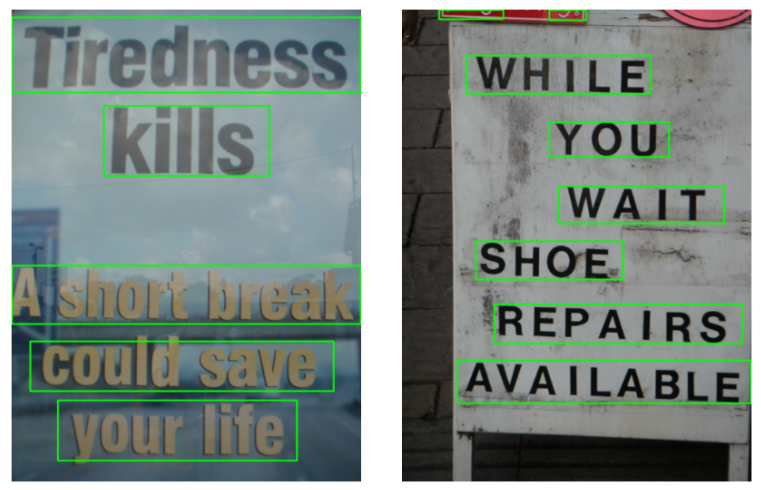
\includegraphics[scale=0.7]{images/text-detection.png}
    \centering
    \caption{Ví dụ về nhiệm vụ phát hiện văn bản}
\end{figure}

Hiện tại, một số thuật toán phát hiện văn bản phổ biến có thể được chia ra một cách đại khái thành hai loại: \textbf{Thuật toán dựa trên Hồi quy} và \textbf{Thuật toán dựa trên Phân đoạn}. Cũng có một số thuật toán kết hợp cả hai loại này. Các thuật toán dựa trên hồi quy lấy cảm hứng từ các thuật toán phát hiện đối tượng chung, thực hiện việc hồi quy hộp phát hiện bằng cách đặt các anchor, hoặc thậm chí trực tiếp thực hiện hồi quy điểm ảnh. Loại phương pháp này hoạt động tốt trong việc phân biệt văn bản có hình dạng đều đặn, nhưng kém trong việc phát hiện văn bản có hình dạng không đều. Ví dụ, CTPN tốt trong việc nhận dạng văn bản ngang, nhưng kém trong việc phát hiện văn bản uốn cong và xoắn. SegLink phù hợp hơn với văn bản dài, nhưng không thích hợp cho việc phát hiện văn bản phân tán thưa thớt. Các thuật toán dựa trên phân đoạn giới thiệu Mask-RCNN, loại thuật toán này có thể hoạt động tốt hơn trong việc phát hiện trong các tình huống và văn bản có các hình dạng khác nhau, nhưng hạn chế là việc xử lý sau cùng phức tạp, vì vậy có thể chậm về tốc độ và không thể phát hiện được văn bản chồng lấn \cite{Dive-into-ocr-2022}.

\begin{figure}[h]
    \tikzset{every picture/.style={line width=0.75pt}} %set default line width to 0.75pt        
\begin{tikzpicture}[x=0.75pt,y=0.75pt,yscale=-1,xscale=1]
    %uncomment if require: \path (0,783); %set diagram left start at 0, and has height of 783

    %Rounded Rect [id:dp12536916830339373] 
    \draw  [color={rgb, 255:red, 246; green, 35; blue, 35 }  ,draw opacity=1 ][fill={rgb, 255:red, 246; green, 35; blue, 35 }  ,fill opacity=1 ] (79.8,126.47) .. controls (79.8,120.47) and (84.67,115.6) .. (90.67,115.6) -- (238.49,115.6) .. controls (244.5,115.6) and (249.37,120.47) .. (249.37,126.47) -- (249.37,159.1) .. controls (249.37,165.1) and (244.5,169.97) .. (238.49,169.97) -- (90.67,169.97) .. controls (84.67,169.97) and (79.8,165.1) .. (79.8,159.1) -- cycle ;
    %Straight Lines [id:da35079927471568495] 
    \draw    (484.18,93.97) -- (484.52,110.57) ;
    \draw [shift={(484.58,113.57)}, rotate = 268.83] [fill={rgb, 255:red, 0; green, 0; blue, 0 }  ][line width=0.08]  [draw opacity=0] (8.93,-4.29) -- (0,0) -- (8.93,4.29) -- cycle    ;
    %Straight Lines [id:da3515453488418392] 
    \draw    (484.18,93.97) -- (164.67,93.67) ;
    %Straight Lines [id:da8167979499170375] 
    \draw    (164.67,93.67) -- (164.67,111.07) ;
    \draw [shift={(164.67,114.07)}, rotate = 270] [fill={rgb, 255:red, 0; green, 0; blue, 0 }  ][line width=0.08]  [draw opacity=0] (8.93,-4.29) -- (0,0) -- (8.93,4.29) -- cycle    ;
    %Straight Lines [id:da24241956645024332] 
    \draw    (324.61,75.97) -- (324.42,93.82) ;
    %Rounded Rect [id:dp4800123674594827] 
    \draw  [color={rgb, 255:red, 0; green, 33; blue, 205 }  ,draw opacity=1 ][fill={rgb, 255:red, 0; green, 33; blue, 205 }  ,fill opacity=1 ] (399.8,125.67) .. controls (399.8,119.67) and (404.67,114.8) .. (410.67,114.8) -- (558.49,114.8) .. controls (564.5,114.8) and (569.37,119.67) .. (569.37,125.67) -- (569.37,158.3) .. controls (569.37,164.3) and (564.5,169.17) .. (558.49,169.17) -- (410.67,169.17) .. controls (404.67,169.17) and (399.8,164.3) .. (399.8,158.3) -- cycle ;
    %Rounded Rect [id:dp7078369789993373] 
    \draw  [color={rgb, 255:red, 36; green, 159; blue, 255 }  ,draw opacity=1 ][fill={rgb, 255:red, 255; green, 255; blue, 255 }  ,fill opacity=0 ] (242.2,31.67) .. controls (242.2,25.67) and (247.07,20.8) .. (253.07,20.8) -- (400.89,20.8) .. controls (406.9,20.8) and (411.77,25.67) .. (411.77,31.67) -- (411.77,64.3) .. controls (411.77,70.3) and (406.9,75.17) .. (400.89,75.17) -- (253.07,75.17) .. controls (247.07,75.17) and (242.2,70.3) .. (242.2,64.3) -- cycle ;
    %Rounded Rect [id:dp5367367596794104] 
    \draw  [fill={rgb, 255:red, 255; green, 255; blue, 255 }  ,fill opacity=0 ][dash pattern={on 4.5pt off 4.5pt}] (22.33,240.83) .. controls (22.33,209.04) and (48.1,183.27) .. (79.89,183.27) -- (252.57,183.27) .. controls (284.36,183.27) and (310.13,209.04) .. (310.13,240.83) -- (310.13,489.65) .. controls (310.13,521.44) and (284.36,547.21) .. (252.57,547.21) -- (79.89,547.21) .. controls (48.1,547.21) and (22.33,521.44) .. (22.33,489.65) -- cycle ;
    %Rounded Rect [id:dp2663541401208218] 
    \draw  [fill={rgb, 255:red, 255; green, 255; blue, 255 }  ,fill opacity=0 ][dash pattern={on 4.5pt off 4.5pt}] (342.33,237.83) .. controls (342.33,206.04) and (368.1,180.27) .. (399.89,180.27) -- (572.57,180.27) .. controls (604.36,180.27) and (630.13,206.04) .. (630.13,237.83) -- (630.13,486.65) .. controls (630.13,518.44) and (604.36,544.21) .. (572.57,544.21) -- (399.89,544.21) .. controls (368.1,544.21) and (342.33,518.44) .. (342.33,486.65) -- cycle ;


    % Text Node
    \draw (42,364.54) node [anchor=north west][inner sep=0.75pt]   [align=left] {\textcolor[rgb]{0,0.09,0.75}{Ưu: Thường tốt cho văn bản }\\\textcolor[rgb]{0,0.09,0.75}{hình dạng thông thường.}\\\textcolor[rgb]{0,0.09,0.75}{Nhược: \ Không được chính xác}\\\textcolor[rgb]{0,0.09,0.75}{khi phát hiện văn bản có hình dạng}\\\textcolor[rgb]{0,0.09,0.75}{ bất thường}};
    % Text Node
    \draw (282.8,46.8) node [anchor=north west][inner sep=0.75pt]   [align=left] {{\small \textbf{phát hiện}}};
    % Text Node
    \draw (270.85,32.97) node [anchor=north west][inner sep=0.75pt]   [align=left] {{\small \textbf{Các thuật toán}}};
    % Text Node
    \draw (104.35,135.57) node [anchor=north west][inner sep=0.75pt]   [align=left] {{\small \textcolor[rgb]{1,1,1}{Dựa trên hồi quy}}};
    % Text Node
    \draw (423.47,135.37) node [anchor=north west][inner sep=0.75pt]   [align=left] {{\small \textcolor[rgb]{1,1,1}{Dựa trên phân vùng}}};
    % Text Node
    \draw (84,208.33) node [anchor=north west][inner sep=0.75pt]   [align=left] {CTPN\\Textboxes/Texboxes++\\EAST\\CRAFT\\...};
    % Text Node
    \draw (404,207.67) node [anchor=north west][inner sep=0.75pt]   [align=left] {Pixel embeding\\PSENet\\PAN\\DB/DB++\\...};
    % Text Node
    \draw (363,361.54) node [anchor=north west][inner sep=0.75pt]   [align=left] {\textcolor[rgb]{0,0.09,0.75}{Ưu: Xử lý tốt với văn bản có hình }\\\textcolor[rgb]{0,0.09,0.75}{dạng khác nhau.}\\\textcolor[rgb]{0,0.09,0.75}{Nhược: \ Quá trình hậu xử lý phức}\\\textcolor[rgb]{0,0.09,0.75}{tạp, tốn thời gian và hiệu quả kém}\\\textcolor[rgb]{0,0.09,0.75}{với văn bản chồng chéo}};
\end{tikzpicture}
    \centering
    \caption{Tổng quan về thuật toán phát hiện văn bản}
\end{figure}

\subsection{Nhận dạng văn bản}
Nhận dạng văn bản là việc nhận biết nội dung văn bản trong hình ảnh, và đầu vào thường là từ phần vùng chứa văn bản của ảnh được cắt ra bằng hộp văn bản được tạo ra từ việc phát hiện văn bản. Nhận dạng văn bản có thể được chia thành hai loại chính: \textbf{Nhận dạng Văn bản Đều đặn} và \textbf{Nhận dạng Văn bản Không đều đặn} dựa trên đường viền của văn bản cần nhận dạng.

\begin{figure}[h]
    
\includegraphics[scale=0.4]{images/regular-irregular-text.png}
    \centering
    \caption{Văn bản đều đặn (trái) và Văn bản không đều đặn (phải)}
\end{figure}

Văn bản đều đặn chủ yếu đề cập đến các phông chữ in, văn bản được quét, và các nguồn tương tự có hướng chính đều. Văn bản không đều đặn thường không nằm trong tư thế ngang, thường uốn cong, bị che khuất và mờ mờ. Các tình huống văn bản không đều đặn thách thức rất lớn, và đó cũng là hướng nghiên cứu chính trong việc nhận dạng văn bản.

Các thuật toán nhận dạng văn bản đều đặn có thể được chia thành hai loại dựa trên các phương pháp giải mã khác nhau: Thuật toán dựa trên CTC và Thuật toán dựa trên Sequence2Sequence. Chúng khác nhau trong cách chuyển đổi các đặc trưng chuỗi mà mạng học học được thành kết quả nhận dạng cuối cùng. Một ví dụ đại diện cho thuật toán dựa trên CTC là CRNN cổ điển.

\begin{figure}[p]
    \tikzset{every picture/.style={line width=0.75pt}} %set default line width to 0.75pt        

\begin{tikzpicture}[x=0.75pt,y=0.75pt,yscale=-1,xscale=1]
    %uncomment if require: \path (0,819); %set diagram left start at 0, and has height of 819

    %Rounded Rect [id:dp7357497005786489] 
    \draw  [dash pattern={on 4.5pt off 4.5pt}] (78.38,111.44) .. controls (78.38,78.6) and (105,51.98) .. (137.84,51.98) -- (484.66,51.98) .. controls (517.5,51.98) and (544.12,78.6) .. (544.12,111.44) -- (544.12,289.82) .. controls (544.12,322.66) and (517.5,349.28) .. (484.66,349.28) -- (137.84,349.28) .. controls (105,349.28) and (78.38,322.66) .. (78.38,289.82) -- cycle ;
    %Up Down Arrow [id:dp10182102951041139] 
    \draw  [color={rgb, 255:red, 0; green, 0; blue, 0 }  ,draw opacity=0 ][fill={rgb, 255:red, 255; green, 0; blue, 0 }  ,fill opacity=1 ] (206.27,365.77) -- (220.2,357.52) -- (234.13,365.77) -- (227.16,365.77) -- (227.16,382.27) -- (234.13,382.27) -- (220.2,390.52) -- (206.27,382.27) -- (213.23,382.27) -- (213.23,365.77) -- cycle ;
    %Up Down Arrow [id:dp6666173009893719] 
    \draw  [color={rgb, 255:red, 0; green, 0; blue, 0 }  ,draw opacity=0 ][fill={rgb, 255:red, 255; green, 0; blue, 0 }  ,fill opacity=1 ] (406.67,365.77) -- (420.6,357.52) -- (434.53,365.77) -- (427.56,365.77) -- (427.56,382.27) -- (434.53,382.27) -- (420.6,390.52) -- (406.67,382.27) -- (413.63,382.27) -- (413.63,365.77) -- cycle ;
    %Rounded Rect [id:dp06853301880737295] 
    \draw  [dash pattern={on 4.5pt off 4.5pt}] (77.38,457.44) .. controls (77.38,424.6) and (104,397.98) .. (136.84,397.98) -- (483.66,397.98) .. controls (516.5,397.98) and (543.12,424.6) .. (543.12,457.44) -- (543.12,635.82) .. controls (543.12,668.66) and (516.5,695.28) .. (483.66,695.28) -- (136.84,695.28) .. controls (104,695.28) and (77.38,668.66) .. (77.38,635.82) -- cycle ;

    % Text Node
    \draw (222,465.41) node   [align=left] {\begin{minipage}[lt]{68pt}\setlength\topsep{0pt}
            CRNN\\STAR-Net\\Rosetta\\...
        \end{minipage}};
    % Text Node
    \draw (407,465.91) node   [align=left] {\begin{minipage}[lt]{68pt}\setlength\topsep{0pt}
            R2AM\\SAR\\RARE\\...
        \end{minipage}};
    % Text Node
    \draw (209.63,593.06) node   [align=left] {\begin{minipage}[lt]{134.82pt}\setlength\topsep{0pt}
            \textcolor[rgb]{0,0.45,0.08}{Ưu: Hiệu quả cao, tốt cho văn bản thông thường và dài}\\\textcolor[rgb]{1,0,0}{Nhược: Không sử dụng thông tin ngữ cảnh}
        \end{minipage}};
    % Text Node
    \draw (419.63,581.49) node   [align=left] {\begin{minipage}[lt]{134.82pt}\setlength\topsep{0pt}
            \textcolor[rgb]{0,0.45,0.08}{Ưu: Độ chính xác cao}\\\textcolor[rgb]{1,0,0}{Nhược: Hiệu quả kém cho văn bản quá dài hoặc quá ngắn}
        \end{minipage}};
    % Text Node
    \draw  [color={rgb, 255:red, 74; green, 144; blue, 226 }  ,draw opacity=1 ]  (247.07,78.7) .. controls (247.07,69.86) and (254.24,62.7) .. (263.07,62.7) -- (346.07,62.7) .. controls (354.91,62.7) and (362.07,69.86) .. (362.07,78.7) -- (362.07,92.7) .. controls (362.07,101.53) and (354.91,108.7) .. (346.07,108.7) -- (263.07,108.7) .. controls (254.24,108.7) and (247.07,101.53) .. (247.07,92.7) -- cycle  ;
    \draw (304.57,85.7) node   [align=left] {\begin{minipage}[lt]{75.58pt}\setlength\topsep{0pt}
            \begin{center}
                Thuật toán nhận dạng
            \end{center}

        \end{minipage}};
    % Text Node
    \draw  [color={rgb, 255:red, 0; green, 0; blue, 0 }  ,draw opacity=0 ][fill={rgb, 255:red, 145; green, 9; blue, 181 }  ,fill opacity=1 ]  (158.74,151.2) .. controls (158.74,142.37) and (165.9,135.2) .. (174.74,135.2) -- (257.74,135.2) .. controls (266.58,135.2) and (273.74,142.37) .. (273.74,151.2) -- (273.74,167.2) .. controls (273.74,176.04) and (266.58,183.2) .. (257.74,183.2) -- (174.74,183.2) .. controls (165.9,183.2) and (158.74,176.04) .. (158.74,167.2) -- cycle  ;
    \draw (216.24,159.2) node  [color={rgb, 255:red, 255; green, 255; blue, 255 }  ,opacity=1 ] [align=left] {\begin{minipage}[lt]{75.58pt}\setlength\topsep{0pt}
            \begin{center}
                CTC-based
            \end{center}

        \end{minipage}};
    % Text Node
    \draw  [color={rgb, 255:red, 0; green, 0; blue, 0 }  ,draw opacity=0 ][fill={rgb, 255:red, 0; green, 81; blue, 33 }  ,fill opacity=1 ]  (347.41,152.04) .. controls (347.41,143.2) and (354.57,136.04) .. (363.41,136.04) -- (446.41,136.04) .. controls (455.24,136.04) and (462.41,143.2) .. (462.41,152.04) -- (462.41,166.04) .. controls (462.41,174.88) and (455.24,182.04) .. (446.41,182.04) -- (363.41,182.04) .. controls (354.57,182.04) and (347.41,174.88) .. (347.41,166.04) -- cycle  ;
    \draw (404.91,159.04) node  [color={rgb, 255:red, 255; green, 255; blue, 255 }  ,opacity=1 ] [align=left] {\begin{minipage}[lt]{75.58pt}\setlength\topsep{0pt}
            \begin{center}
                Attention-based
            \end{center}

        \end{minipage}};
    % Text Node
    \draw (146.33,205.31) node [anchor=north west][inner sep=0.75pt]   [align=left] {\mbox{-} CRNN+CTC\\\mbox{-} Giới thiệu một ký tự không \\gian\\\mbox{-} Nhãn không yêu cầu căn \\chỉnh cấp độ ký tự};
    % Text Node
    \draw (337,206.33) node [anchor=north west][inner sep=0.75pt]   [align=left] {\mbox{-} Seq2Seq+attention};
    % Connection
    \draw    (276.93,108.7) -- (246.62,133.92) ;
    \draw [shift={(245.08,135.2)}, rotate = 320.24] [color={rgb, 255:red, 0; green, 0; blue, 0 }  ][line width=0.75]    (10.93,-3.29) .. controls (6.95,-1.4) and (3.31,-0.3) .. (0,0) .. controls (3.31,0.3) and (6.95,1.4) .. (10.93,3.29)   ;
    % Connection
    \draw    (336.04,108.7) -- (371.83,134.86) ;
    \draw [shift={(373.44,136.04)}, rotate = 216.17] [color={rgb, 255:red, 0; green, 0; blue, 0 }  ][line width=0.75]    (10.93,-3.29) .. controls (6.95,-1.4) and (3.31,-0.3) .. (0,0) .. controls (3.31,0.3) and (6.95,1.4) .. (10.93,3.29)   ;

\end{tikzpicture}
    \centering
    \caption{CTC-based recognition algorithm VS. Attention-based recognition algorithm}
\end{figure}

Các thuật toán nhận dạng cho văn bản không đều đặn phong phú hơn. Các phương pháp như STAR-Net sửa chữa đường viền của văn bản không đều đặn thành các hình chữ nhật đều đặn bằng cách thêm các mô-đun sửa chữa như TPS trước khi thực hiện việc nhận dạng. Các phương pháp dựa trên chú ý như RARE chú trọng hơn đến mối quan hệ giữa các phần trong chuỗi. Các phương pháp dựa trên phân đoạn xử lý mỗi ký tự trên dòng văn bản như một đơn vị riêng lẻ, làm cho việc nhận dạng ký tự đã phân đoạn dễ dàng hơn so với việc nhận dạng toàn bộ dòng văn bản sau khi sửa chữa. Ngoài ra, với sự phát triển nhanh chóng của Transformer và hiệu quả đã được xác minh trong các nhiệm vụ khác nhau trong những năm gần đây, nhiều thuật toán nhận dạng văn bản dựa trên transformer đã phát triển mạnh mẽ. Loại giải pháp này sử dụng cấu trúc transformer để giải quyết việc mô hình hóa sự phụ thuộc lâu dài trong CNN và đã đạt được kết quả tốt.

\begin{figure}
    
\includegraphics[scale=0.35]{images/recognition-based-charcter-segmentation.png}
    \centering
    \caption{Thuật toán nhận dạng dựa trên phân vùng ký tự}
\end{figure}

\subsection{Nhận dạng cấu trúc tài liệu}
Công nghệ OCR có thể đáp ứng yêu cầu về phát hiện và nhận dạng văn bản. Tuy nhiên, trong các tình huống thực tế, điều chúng ta thường cần là thông tin có cấu trúc, chẳng hạn như trích xuất thông tin từ thẻ ID và hóa đơn, xác định có cấu trúc của bảng, và vân vân. Các tình huống ứng dụng của công nghệ OCR chủ yếu là trích xuất tài liệu nhanh, so sánh nội dung hợp đồng, so sánh thông tin tài chính trên các tài liệu cần thanh toán, và xác định tài liệu vận chuyển. Kết quả OCR + xử lý sau cùng là một kế hoạch cấu trúc thường được sử dụng, nhưng phức tạp và cần thiết phải được thiết kế cẩn thận, và thiếu sự tổng quát. Với sự phát triển liên tục của công nghệ OCR và nhu cầu về trích xuất thông tin có cấu trúc đang gia tăng, các công nghệ liên quan đến phân tích tài liệu thông minh, như phân tích bố cục, nhận dạng bảng, và trích xuất thông tin quan trọng, đã nhận được sự chú ý ngày càng tăng.

\subsubsection*{Phân tích bố cục}
Phân tích bố cục được thực hiện để phân loại nội dung của hình ảnh tài liệu thành các loại như văn bản thuần túy, tiêu đề, bảng biểu, hình ảnh, v.v. Các phương pháp hiện tại thường thực hiện việc phát hiện hoặc phân đoạn chúng một cách riêng biệt. Ví dụ, Soto Carlos sử dụng thông tin ngữ cảnh và vị trí tự nhiên của nội dung tài liệu để cải thiện hiệu suất phát hiện vùng dựa trên thuật toán phát hiện mục tiêu Faster R-CNN. Sarkar Mausoom và đồng nghiệp đề xuất một cơ chế phân đoạn dựa trên tiên biết để huấn luyện mô hình phân đoạn tài liệu với các hình ảnh có độ phân giải cao, giải quyết vấn đề rằng các cấu trúc khác nhau trong các khu vực dày đặc không thể phân biệt và hợp nhất do việc giảm quá mức của hình ảnh gốc.

\subsubsection*{Nhận dạng bảng}
Nhận dạng bảng là việc xác định và chuyển thông tin bảng của tài liệu thành một tệp Excel. Có nhiều loại và phong cách bảng khác nhau trong hình ảnh văn bản, chẳng hạn như các hàng và cột khác nhau và các loại văn bản khác nhau. Ngoài ra, phong cách của tài liệu và môi trường ánh sáng khi chụp ảnh đã đặt ra những thách thức lớn cho việc nhận dạng bảng, làm cho việc nhận dạng bảng trở thành một vấn đề nghiên cứu khó khăn trong việc hiểu tài liệu. Có nhiều phương pháp nhận dạng bảng. Ví dụ, vào những ngày đầu tiên, có các thuật toán truyền thống dựa trên các quy tắc heuristics, như thuật toán T-Rect được đề xuất bởi Kieninger và cộng sự, thường sử dụng quy tắc thiết kế thủ công và phát hiện và phân tích miền kết nối. Trong những năm gần đây, khi học sâu tiếp tục phát triển, một số thuật toán nhận dạng cấu trúc bảng dựa trên mạng CNN đã xuất hiện, như DeepTabStR được đề xuất bởi Siddiqui Shoaib Ahmed và cộng sự và TabStruct-Net được đề xuất bởi Raja Sachin và cộng sự. Ngoài ra, với sự gia tăng của Mạng Neural Đồ thị, một số nhà nghiên cứu đã thử áp dụng Mạng Neural Đồ thị vào việc nhận dạng cấu trúc bảng và coi việc nhận dạng bảng như một vấn đề tái tạo đồ thị dựa trên Mạng Neural Đồ thị. Đây là cách mà TGRNet được đề xuất bởi Xue Wenyuan và cộng sự hoạt động. Hơn nữa, có các giải pháp end-to-end có kết quả đầu ra cấu trúc bảng dưới dạng HTML bằng mạng. Hầu hết trong số này áp dụng Seq2Seq để dự đoán cấu trúc bảng như những thuật toán dựa trên attention hoặc transformer, bao gồm TableMaster.

\subsubsection*{Trích xuất thông tin chính}
Trích xuất thông tin quan trọng (KIE) là một nhiệm vụ quan trọng trong Hỏi và Trả lời Văn bản (Document VQA). Nó liên quan đến việc trích xuất thông tin cần thiết từ hình ảnh, chẳng hạn như tên và số ID từ thẻ ID. Thông tin như vậy thường được xác định trong một nhiệm vụ, nhưng khác nhau giữa các nhiệm vụ khác nhau.

\begin{figure}[h!]
    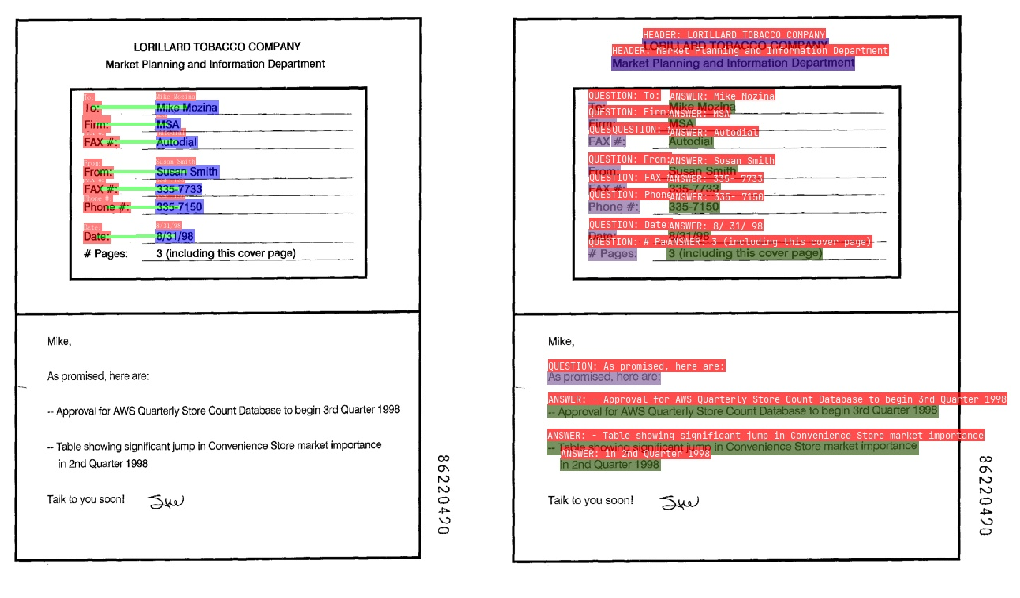
\includegraphics[scale=0.56]{images/re-vs-ser.png}
    \centering
    \caption{RE(trái) VS SER(phải)}
    \label{fig8:ser-re}
\end{figure}

KIE thường được chia thành hai phần nhiệm vụ con để nghiên cứu (Hình \ref{fig8:ser-re}):
\begin{itemize}
    \item SER: Đây là việc nhận dạng thực thể ngữ nghĩa, phân loại từng đoạn văn bản được phát hiện. Ví dụ, nó chia văn bản thành tên và số thẻ ID như hình dưới đây.
    \item RE: Đây là việc trích xuất mối quan hệ, phân loại từng đoạn văn bản. Ví dụ, nó có thể phân loại văn bản thành câu hỏi và câu trả lời, sau đó tìm câu trả lời tương ứng cho mỗi câu hỏi. Như hình dưới đây, các hộp đỏ và đen đại diện cho câu hỏi và câu trả lời tương ứng, và các mũi tên màu vàng chỉ sự tương ứng giữa câu hỏi và câu trả lời.
\end{itemize}
Phương pháp KIE thông thường được phát triển dựa trên nhận dạng thực thể đặt tên (NER), nhưng loại phương pháp này chỉ sử dụng thông tin văn bản trong hình ảnh mà không sử dụng thông tin hình ảnh và cấu trúc. Do đó, nó không đạt độ chính xác cao. Trong những năm gần đây, nhiều giải pháp đã bắt đầu kết hợp thông tin hình ảnh và cấu trúc với thông tin văn bản. Do sử dụng các nguyên tắc khác nhau trong việc kết hợp thông tin đa tầng, các phương pháp này có thể được chia thành bốn loại:
\begin{itemize}
    \item Phương pháp dựa trên lưới
    \item Phương pháp dựa trên token
    \item Phương pháp dựa trên Graph Convolutional Network
    \item Phương pháp end-to-end
\end{itemize}

\section{OCR dựa trên mẫu và OCR dựa trên AI}
Với số lượng ngày càng tăng của các giải pháp OCR có sẵn trên thị trường, điều cần thiết là phải hiểu các kỹ thuật chính được sử dụng bởi các công cụ này, cụ thể là OCR dựa trên mẫu và OCR dựa trên AI.
\subsection{OCR dựa trên mẫu}
OCR dựa trên mẫu là một cách tiếp cận cũ hơn, truyền thống hơn đối với OCR dựa trên các mẫu được xác định trước để nhận dạng và trích xuất văn bản từ tài liệu. Phương pháp này hoạt động tốt nhất khi xử lý các tài liệu có cấu trúc, chẳng hạn như hóa đơn, biểu mẫu hoặc biên lai, có bố cục nhất quán. \cite{template-ai-ocr}
\begin{itemize}
    \item[] \textbf{Ưu điểm:} \begin{enumerate}
            \item Độ chính xác cao: Khi được sử dụng với các tài liệu có cấu trúc tuân theo định dạng nhất định, OCR dựa trên mẫu có thể đạt được tỷ lệ chính xác tuyệt vời.
            \item Thời gian xử lý thấp hơn: Vì OCR dựa trên mẫu dựa trên các mẫu dựng sẵn, nó không yêu cầu nhiều sức mạnh xử lý hoặc thời gian để nhận dạng ký tự.
            \item Có thể tùy chỉnh: Người dùng có thể tạo các mẫu tùy chỉnh cho các loại tài liệu cụ thể, đảm bảo kết quả chính xác.
        \end{enumerate}
    \item[] \textbf{Nhược điểm} \begin{enumerate}
            \item Tính linh hoạt hạn chế: OCR dựa trên mẫu gặp khó khăn khi xử lý các tài liệu không tuân theo định dạng nhất quán hoặc có bố cục phức tạp.
            \item Thiết lập tốn thời gian: Tạo các mẫu tùy chỉnh có thể là một quá trình tẻ nhạt, đặc biệt là khi xử lý nhiều loại tài liệu.
            \item Không hiệu quả đối với văn bản viết tay: OCR dựa trên mẫu thường hoạt động kém khi xử lý văn bản viết tay hoặc phông chữ.
        \end{enumerate}
\end{itemize}

Các trường hợp sử dụng tốt nhất cho OCR dựa trên mẫu: Cách tiếp cận này phù hợp nhất với các tổ chức xử lý khối lượng lớn tài liệu có cấu trúc với bố cục nhất quán, chẳng hạn như hóa đơn hoặc biểu mẫu.

\subsection{OCR Dựa trên AI}
OCR dựa trên AI tận dụng trí tuệ nhân tạo, máy học và mạng thần kinh để nhận dạng và trích xuất văn bản từ tài liệu. Cách tiếp cận này nâng cao hơn và có thể xử lý nhiều loại tài liệu, bao gồm cả tài liệu phi cấu trúc và bán cấu trúc. \cite{template-ai-ocr}
\begin{itemize}
    \item[] \textbf{Ưu điểm:} \begin{enumerate}
            \item Độ chính xác và tính linh hoạt cao: OCR dựa trên AI có thể thích ứng với nhiều loại tài liệu và bố cục khác nhau, mang lại kết quả chính xác ngay cả khi xử lý các bố cục phức tạp hoặc không nhất quán.
            \item Xử lý văn bản viết tay: OCR dựa trên AI được trang bị tốt hơn để nhận dạng và trích xuất phông chữ văn bản viết tay hoặc tập lệnh, làm cho nó linh hoạt hơn so với OCR dựa trên mẫu.
            \item Cải tiến liên tục: Các thuật toán máy học cho phép OCR dựa trên AI cải thiện độ chính xác của nó theo thời gian khi nó xử lý nhiều tài liệu hơn.
            \item Thiết lập nhanh hơn: OCR dựa trên AI không yêu cầu tạo mẫu tùy chỉnh, cho phép triển khai nhanh hơn.
        \end{enumerate}
    \item[] \textbf{Nhược điểm} \begin{enumerate}
            \item Thời gian xử lý cao hơn: OCR dựa trên AI thường yêu cầu nhiều thời gian và sức mạnh xử lý hơn so với OCR dựa trên mẫu, vì nó phân tích tài liệu toàn diện hơn.
            \item Chi phí cao hơn: Các giải pháp OCR dựa trên AI có thể đắt hơn do công nghệ tiên tiến và sự phát triển liên tục có liên quan.

        \end{enumerate}
\end{itemize}

Các trường hợp sử dụng tốt nhất cho OCR dựa trên AI: Phương pháp này lý tưởng cho các tổ chức xử lý nhiều loại tài liệu, bao gồm cả tài liệu phi cấu trúc và bán cấu trúc hoặc yêu cầu trích xuất văn bản viết tay

\section{Học sâu}
Trong việc ứng dụng OCR để nhận dạng hóa đơn, mạng học sâu đã chơi một vai trò quan trọng và mang lại những cải tiến đáng kể cho quá trình này. Trước khi sự xuất hiện của học sâu, các hệ thống nhận dạng dựa trên các phương pháp truyền thống thường gặp khó khăn trong việc xử lý các biến thể phức tạp của hình ảnh hóa đơn và khả năng xử lý đa dạng của chúng. Nhưng với mạng nơron học sâu, khả năng học và tự điều chỉnh của mô hình đã mở ra những cánh cửa mới cho việc nhận dạng hóa đơn hiệu quả hơn.

\subsection{Học sâu là gì?}
Học sâu là một các tiếp cận của Trí tuệ nhân tạo. Cụ thể thì nó là một kiểu của học máy (Hình \ref{fig:venn1}), một kỹ thuật mà cho phép hệ thống máy tính tự học từ trải nghiệm và dữ liệu, nó sở hữu sức mạnh và sự linh hoạt tuyệt vời thông qua việc học cách biểu diễn như một hệ phân cấp khái niệm trong đó mỗi khái niệm được định nghĩa từ những khái niệm đơn giản hơn, và mỗi biểu diễn được tính tính toán từ những biểu diễn kém trừu tượng hơn. \cite{Goodfellow-et-al-2016}

\begin{figure}
    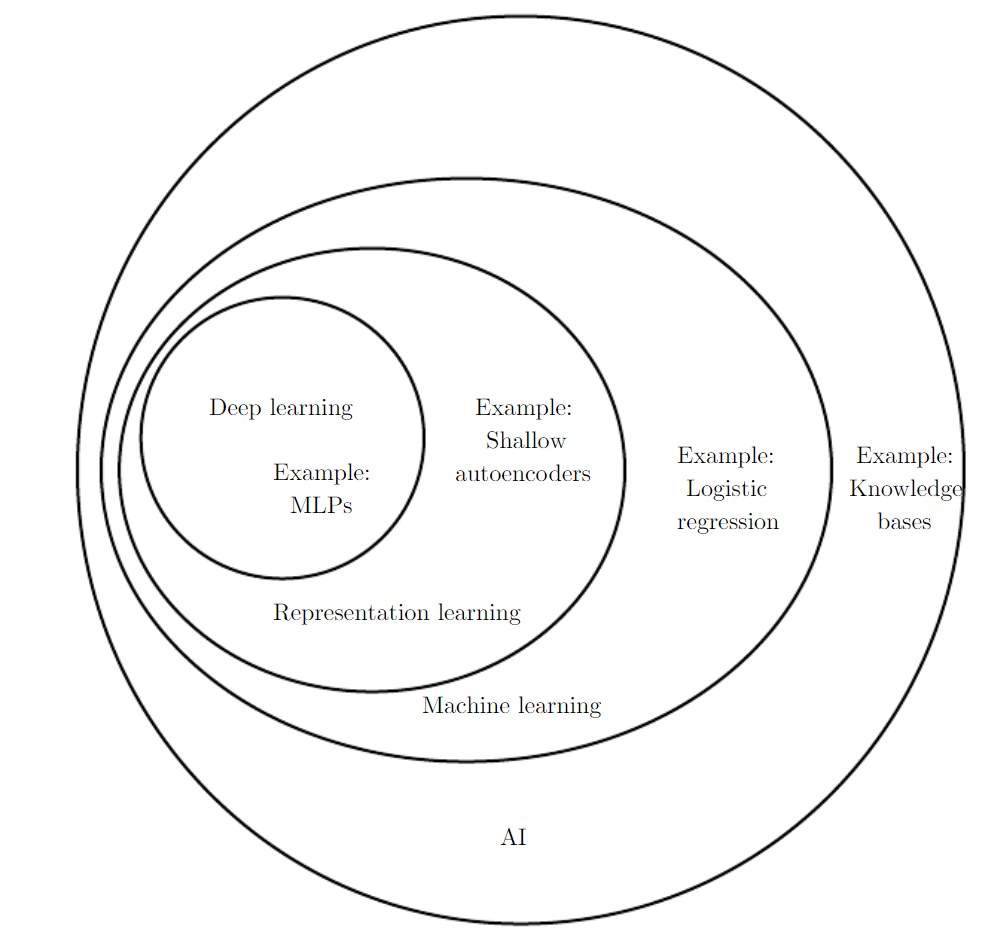
\includegraphics[scale=0.45]{images/venn_diagram_deeplearning.png}
    \centering
    \caption{Biểu đồ Venn về Trí tuệ nhân tạo}
    \label{fig:venn1}
\end{figure}


Một điểm đáng chú ý là học sâu cần một lượng lớn dữ liệu để huấn luyện mô hình một cách hiệu quả \cite{wiki-deep-learning}. Trong trường hợp OCR và nhận dạng hóa đơn, mạng nơron học sâu có khả năng học từ hàng nghìn hoặc thậm chí hàng triệu hình ảnh hóa đơn, điều này giúp mô hình hiểu rõ các đặc trưng và biểu diễn của dữ liệu hơn.

Hiện nay các kiến trúc học sâu như mạng nơ-ron sâu, mạng niềm tin sâu, học tăng cường sâu, mạng nơ-ron tái phát, mạng nơ-ron tích chập và máy biến áp đã được áp dụng cho các lĩnh vực bao gồm thị giác máy tính, nhận dạng giọng nói, xử lý ngôn ngữ tự nhiên, dịch máy, tin sinh học, thiết kế thuốc, Phân tích hình ảnh y tế, khoa học khí hậu, kiểm tra vật liệu và các chương trình trò chơi trên bàn cờ, nơi chúng đã tạo ra kết quả tương đương và trong một số trường hợp vượt qua hiệu suất chuyên gia của con người.

\subsection{Kiến trúc mạng nơ-ron nhân tạo}
Mạng nơ-ron nhân tạo là một mô hình được lấy cảm hứng từ mạng nơ-ron thần kinh. Kết hợp với các kĩ thuật học sâu, nó đang trở thành một công cụ rất mạnh mẽ mang lại hiệu quả tốt nhất cho nhiều bài toán khó như nhận dạng ảnh, giọng nói hay xử lý ngôn ngữ tự nhiên. Một mạng nơ-ron được cấu thành bởi các nơ-ron đơn lẻ được gọi là các perceptron.

Một perceptron sẽ nhận một hoặc nhiều đầu $\mathbf{x}$ vào dạng nhị phân và cho ra một kết quả $o$ dạng nhị phân duy nhất. Các đầu vào được điều phối tầm ảnh hưởng bởi các tham số trọng lượng tương ứng $\mathbf{w}$ của nó, còn kết quả đầu ra được quyết định dựa vào một ngưỡng quyết định $b$ nào đó:
$$o = \begin{cases}
        0 & \text{if } \sum_i w_i x_i +b \leq 0 \\
        1 & \text{if } \sum_i w_i x_i +b \ge 0
    \end{cases}$$

Mạng nơ-ron là sự kết hợp của của các tầng perceptron hay còn được gọi là perceptron đa tầng như hình vẽ bên dưới:
\begin{figure}[h]
    \begin{tikzpicture}[x=2.2cm,y=1.4cm]
    \message{^^JNeural network with arrows}
    \readlist\Nnod{4,5,5,5,3} % array of number of nodes per layer
    \message{^^J  Layer}
    \foreachitem \N \in \Nnod{ % loop over layers
        \edef\lay{\Ncnt} % alias of index of current layer
        \message{\lay,}
        \pgfmathsetmacro\prev{int(\Ncnt-1)} % number of previous layer
        \foreach \i [evaluate={\y=\N/2-\i; \x=\lay; \n=\nstyle;}] in {1,...,\N}{ % loop over nodes

                % NODES
                \node[node \n] (N\lay-\i) at (\x,\y) {$a_\i^{(\prev)}$};
                %\node[circle,inner sep=2] (N\lay-\i') at (\x-0.15,\y) {}; % shifted node
                %\draw[node] (N\lay-\i) circle (\R);

                % CONNECTIONS
                \ifnum\lay>1 % connect to previous layer
                    \foreach \j in {1,...,\Nnod[\prev]}{ % loop over nodes in previous layer
                            \draw[connect arrow] (N\prev-\j) -- (N\lay-\i); % connect arrows directly
                            %\draw[connect arrow] (N\prev-\j) -- (N\lay-\i'); % connect arrows to shifted node
                        }
                \fi % else: nothing to connect first layer
            }
    }
    % LABELS
    \node[above=5,align=center,mygreen!60!black] at (N1-1.90) {Lớp đầu vào};
    \node[above=2,align=center,myblue!60!black] at (N3-1.90) {Lớp ẩn};
    \node[above=8,align=center,myred!60!black] at (N\Nnodlen-1.90) {Lớp đầu ra};

\end{tikzpicture}
    \centering
    \caption{Kiến trúc một mạng Nơ-ron}

\end{figure}

Một mạng NN sẽ có 3 kiểu tầng \cite{aws-deep-learning}:
\begin{itemize}
    \item \textbf{Lớp đầu vào:} Một mạng nơ-ron nhân tạo sẽ có một số nút để nhập dữ liệu đầu vào. Các nút này tạo nên lớp đầu vào của hệ thống.
    \item \textbf{Lớp ẩn:} Lớp đầu vào xử lý và chuyển dữ liệu đến các lớp sâu hơn trong mạng nơ-ron. Các lớp ẩn này xử lý thông tin ở các cấp độ khác nhau, thích ứng với hành vi của mình khi nhận được thông tin mới. Các mạng học sâu có hàng trăm lớp ẩn có thể được dùng để phân tích một vấn đề từ nhiều góc độ khác nhau.
    \item \textbf{Lớp đầu ra:} Lớp đầu ra bao gồm các nút xuất dữ liệu. Các mô hình học sâu xuất ra đáp án "có" hoặc "không" chỉ có hai nút trong lớp đầu ra. Mặt khác, các mô hình xuất ra nhiều đáp án hơn sẽ có nhiều nút hơn.
\end{itemize}

Trong mạng Nơ-ron, mỗi nút mạng là một sigmoid nơ-ron nhưng hàm kích hoạt của chúng có thể khác nhau. Tuy nhiên trong thực tế người ta thường để chúng cùng dạng với nhau để tính toán cho thuận lợi.

Ở mỗi tầng, số lượng các nút mạng (nơ-ron) có thể khác nhau tuỳ thuộc vào bài toán và cách giải quyết. Nhưng thường khi làm việc người ta để các tầng ẩn có số lượng nơ-ron bằng nhau. Ngoài ra, các nơ-ron ở các tầng thường được liên kết đôi một với nhau tạo thành mạng kết nối đầy đủ. Khi đó ta có thể tính được kích cỡ của mạng dựa vào số tầng và số nơ-ron.

\subsection{ResNet}
ResNet, viết tắt của ``Residual Network'', là một kiến trúc mạng nơ-ron sâu được giới thiệu bởi Kaiming He và đồng nghiệp vào năm 2015. \acrshort*{resnet} đã đạt được thành công lớn trong việc giải quyết vấn đề đào tạo mạng nơ-ron sâu với số lượng lớp ngày càng tăng mà không gặp vấn đề về độ sâu. Kiến trúc của ResNet đã giúp giải quyết vấn đề triệt tiêu gradient và giúp việc huấn luyện mạng nơ-ron sâu trở nên dễ dàng hơn.

Một vấn đề thường gặp khi huấn luyện mạng nơ-ron sâu là hiện tượng triệt tiêu độ dốc (vanishing gradient) và bùng nổ độ dốc(exploding gradient), đặc biệt là khi mạng có nhiều lớp. Điều này dẫn đến khó khăn trong việc lan truyền ngược độ dốc trong quá trình học. ResNet giải quyết vấn đề này bằng cách sử dụng khối ``residual''.

\subsubsection*{Identity Mapping}
Identity mapping hay còn gọi là ánh xạ đồng nhất là một khái niệm quan trọng trong toán học và xử lý tín hiệu, đặc biệt là trong lĩnh vực của mạng nơ-ron và học sâu. Đơn giản, ánh xạ đồng nhất đề cập đến việc ánh xạ một giá trị đầu vào sang giá trị đầu ra mà không thay đổi giá trị hoặc cấu trúc của dữ liệu. Trong các mô hình học sâu, việc sử dụng ánh xạ đồng nhất có thể giúp cho việc huấn luyện mô hình trở nên hiệu quả hơn.

Khi áp dụng trong mạng nơ-ron, ánh xạ đồng nhất thường được sử dụng như là một thành phần của các các khối residual trong kiến trúc ResNet. Trong ResNet cho phép thông tin từ tầng trước được truyền thẳng qua mà không qua bất kỳ biến đổi nào, thông qua phép toán ``identity shortcut''. Điều này giúp cho việc huấn luyện mô hình dễ dàng hơn và cải thiện khả năng học của mạng, đặc biệt là khi mạng trở nên rất sâu \cite{he2016identity}.

\subsubsection*{Residual learning}
Phương pháp tiếp cận này được gọi là ``Residual Learning'' được sử dụng trong việc đào tạo mạng nơ-ron sâu . Thay vì cố gắng trực tiếp xấp xỉ một phép ánh xạ mong muốn $\mathcal{H}(x)$ bằng cách sử dụng các lớp xếp chồng lên nhau, Mô hình đề xuất một phương pháp là xấp xỉ một hàm residual $\mathcal{F}(x)$ là hiệu của $\mathcal{H}(x)$ và đầu vào $x$. Điều này có nghĩa là phép ánh xạ ban đầu $\mathcal{H}(x)$ có thể được xây dựng lại như $\mathcal{F}(x) + x$ \cite{he2015deep}.

Trong \cite{he2015deep} tác giả lập luận rằng vấn đề suy giảm trong mạng sâu, khi mô hình sâu hơn hoạt động kém hơn so với các mô hình nông, có thể do khó khăn trong việc xấp xỉ các phép ánh xạ đông nhất(identity mapping) bằng nhiều lớp phi tuyến. Trong trường hợp các lớp được thêm vào hoạt động như các phép ánh xạ đông nhất, một mạng sâu hơn nên hoạt động ít nhất cũng tốt như một mạng cạn. Tuy nhiên, điều này thường không được quan sát.

Bằng cách sắp xếp lại vấn đề thành việc xấp xỉ một hàm residual, quá trình tối ưu hóa có thể tập trung vào việc điều chỉnh trọng số của các lớp phi tuyến về gần không. Sự sắp xếp lại này cũng giúp trong các trường hợp mà hàm tối ưu gần với phép ánh xạ đồng nhất, làm cho quá trình tối ưu hóa dễ dàng hơn trong việc tìm các biến đổi liên quan đến phép ánh xạ đồng nhất thay vì học một hàm hoàn toàn mới.

\subsubsection{Identity Mapping by Shortcuts}
Residual learning được áp dụng cho một vài lớp xếp chồng lên nhau. Một khối xây dựng minh họa trong Hình \ref{residual-block}. Một cách chính thức, trong bài báo \cite{he2015deep} tác giả xem xét một khối xây dựng được định nghĩa như sau: 
$$\mathbf{y} = \mathcal{F}(\mathbf{x}, \{W_i\}) + \mathbf{x}$$ 
Ở đây $\mathbf{x}$ và $\mathbf{y}$ là vectơ đầu vào và đầu ra của các lớp được xem xét. Hàm $\mathcal{F}(\mathbf{x}, \{W_i\})$ biểu diễn sự ánh xạ dư cần học. Với ví dụ trong Hình \ref{residual-block} có hai lớp, $\mathcal{F} = W_2 \sigma (W_1 \mathbf{x})$ trong đó $\sigma$ biểu thị ReLU. Phép toán $\mathcal{F} + \mathbf{x}$ được thực hiện bởi một kết nối tắt và phép cộng từng phần tử.

\begin{figure}[h]
    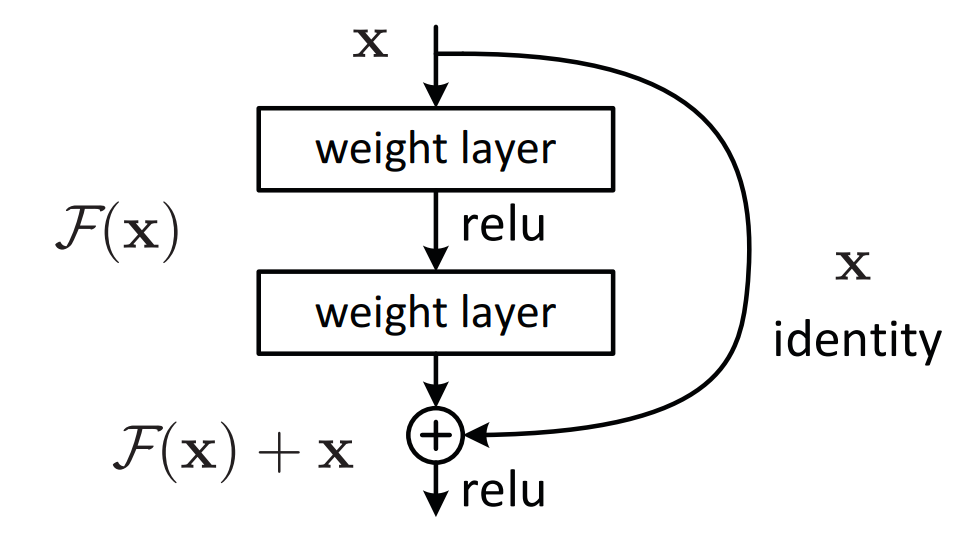
\includegraphics[scale=0.3]{images/residual_block.png}
    \centering
    \caption{Một khối residual}
    \label{residual-block}
\end{figure}

Kết nối tắt thực hiện ánh xạ đồng nhất giữa đầu vào và đầu ra của một khối xây dựng trong mạng thần kinh. Phương trình này không thêm tham số hay phức tạp tính toán. Điều này quan trọng trong so sánh giữa mạng thuần túy và mạng dư thừa. Giúp giải quyết vấn đề suy giảm gradient trong mạng sâu, cho phép huấn luyện hiệu quả mạng sâu hơn.

\subsection{Transformer}
Transformer là một kiến trúc mạng nơ-ron sâu được giới thiệu bởi Vaswani et al. trong bài báo ``Attention Is All You Need \cite{vaswani2023attention}'' vào năm 2017. Đây là một trong những tiến bộ quan trọng trong lĩnh vực xử lý ngôn ngữ tự nhiên và máy dịch dẫn đến những cải tiến đáng kể trong các ứng dụng như dịch máy, tổng hợp văn bản và nhiều nhiệm vụ khác liên quan đến ngôn ngữ.

Kiến trúc Transformer dựa trên cơ chế attention (chú ý), cho phép mạng có khả năng xem xét toàn bộ các phần của dữ liệu đầu vào cùng một lúc, thay vì như các kiến trúc trước đây phải đi qua từng bước theo thứ tự. Kiến trúc này có thể hoạt động với cả dữ liệu tuỳ chỉnh dài ngắn mà không cần giới hạn về chiều dài chuỗi đầu vào.

Transformer bao gồm hai phần chính: Bộ mã hóa (Encoder) và Bộ giải mã (Decoder). Cả hai phần đều sử dụng nhiều lớp tự chú ý (self-attention) để xác định sự quan hệ giữa các phần tử trong chuỗi đầu vào hoặc đầu ra. Sự chú ý tự cho phép mạng tập trung vào các phần tử quan trọng trong chuỗi và hiểu được mối quan hệ giữa chúng.

Transformer đã trở thành cơ sở cho nhiều kiến trúc mạng nơ-ron tiến tiến trong xử lý ngôn ngữ tự nhiên và thậm chí trong các ứng dụng khác như xử lý hình ảnh. Ví dụ nổi tiếng nhất có thể kể đến là ``BERT'' và ``GPT'' , cả hai đều là các biến thể của kiến trúc Transformer và đã đạt được những kết quả ấn tượng trong nhiều nhiệm vụ liên quan đến xử lý ngôn ngữ tự nhiên.

\subsubsection*{Kiến trúc Transformer}
Transformer tuân theo kiến trúc tổng thể này bằng cách sử dụng các lớp tự chú ý xếp chồng và các lớp kết nối đầy đủ theo điểm cho cả bộ mã hóa và bộ giải mã, như được thể hiện ở nửa trái và nửa phải của Hình \ref{fig3}. 
\begin{figure}[h]
    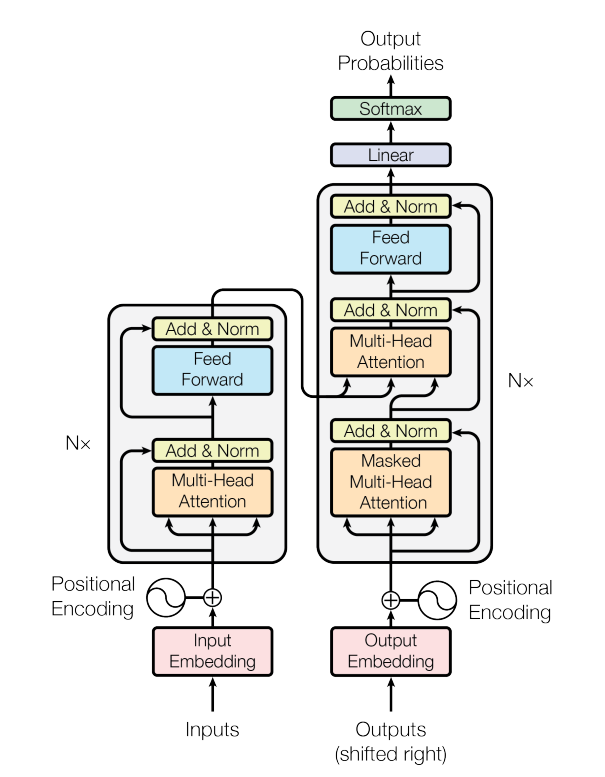
\includegraphics[scale=0.65]{images/transformer-architecture.png}
    \centering
    \caption{Kiến trúc tổng thể của Transformer \cite{vaswani2023attention}}
    \label{fig3}
\end{figure}

\subsubsection*{Ngăn xếp Encoder và Decoder}
\textbf{Bộ mã hóa}: Bộ giải mã có một ngăn xếp gồm $N = 6$ lớp tương tự nhau. Mỗi lớp bao gồm hai lớp con. Lớp đầu tiên là cơ chế  tự chú ý đa đầu(multi-head self-attention), nơi mà mỗi từ trong câu đều ``tương tác'' với tất cả các từ khác để tạo ra sự chú ý chung trong ngữ cảnh. Lớp thứ hai là một mạng truyền thẳng kết nối đầy đủ theo từng vị trí, tức là thông tin từ mỗi vị trí trong câu được xử lý độc lập.

Để duy trì thông tin và hỗ trợ quá trình học, sử dụng kết nối residual xung quanh cả hai lớp con. Kết nối residual cho phép thông tin truyền từ đầu vào của lớp này đến đầu ra một cách dễ dàng. Sau đó, chúng ta thực hiện chuẩn hóa lớp để điều chỉnh phạm vi giá trị đầu ra. Cụ thể, đầu ra của mỗi lớp con được chuẩn hóa thông qua phép tính $\text{LayerNorm}(x + \text{Sublayer}(x))$, trong đó $\text{Sublayer}(x)$ là chức năng được thực hiện bởi chính lớp con đó.

Để đảm bảo tính nhất quán và khả năng kết nối residual, tất cả các lớp con trong mô hình cùng với các lớp nhúng đều tạo ra đầu ra với chiều $d_{model} = 512$, tức là có cùng kích thước đặc trưng để xử lý và truyền thông tin.

\textbf{Bộ giải mã}: Bộ giải mã cũng được tạo thành từ một ngăn xếp gồm $N = 6$ lớp tương tự nhau. Bên cạnh hai lớp con trong mỗi lớp mã hóa, bộ giải mã thêm một lớp con thứ ba, thực hiện chú ý đa đầu (multi-head attention) qua đầu ra của ngăn xếp bộ mã hóa. Tương tự như bộ mã hóa, chúng ta sử dụng kết nối residual xung quanh mỗi lớp con, sau đó là chuẩn hóa lớp. Điều chỉnh lớp con tự chú ý trong ngăn xếp bộ giải mã để ngăn các vị trí tập trung vào các vị trí tiếp theo. Thao tác này, kết hợp với việc lớp nhúng đầu ra được dịch chuyển một vị trí, đảm bảo rằng các dự đoán cho vị trí $i$ chỉ phụ thuộc vào đầu ra đã biết tại các vị trí nhỏ hơn $i$.

\subsubsection*{Attention}
Một hàm chú ý có thể được mô tả như việc ánh xạ một truy vấn và một tập hợp các cặp khóa-giá trị thành một đầu ra, trong đó truy vấn, khóa, giá trị và đầu ra đều là các vector. Đầu ra được tính toán dưới dạng tổng có trọng số của các giá trị, trong đó trọng số được gán cho mỗi giá trị được tính bằng một hàm tương thích của truy vấn với khóa tương ứng.

\subsubsection*{Scaled Dot-Product Attention}
Scaled Dot-Product Attention là một phần quan trọng của kiến trúc Transformer và cơ chế chú ý tự. Đầu vào của phương pháp này gồm các truy vấn (queries) và các khóa (keys) có kích thước $dk$, cùng với các giá trị (values) có kích thước $dv$. Tính tích vô hướng giữa truy vấn và tất cả các khóa, chia từng kết quả cho $dk$, sau đó áp dụng hàm softmax để thu được trọng số cho các giá trị. Thực hiện phép attention trên một tập hợp các truy vấn cùng lúc, gói chúng lại thành một ma trận $Q$. Các khóa và giá trị cũng được gói lại thành các ma trận $K$ và $V$. Kết quả đầu ra được tính bằng cách:
\[
    \text{Attention}(Q, K, V) = \text{softmax} (\frac{ QK^T }{ \sqrt{d_k} }) V   
\]

Bởi vì ảnh hưởng của tích vô hướng trở nên lớn về độ lớn, đẩy hàm softmax vào các vùng có độ dốc rất nhỏ.  Để chống lại tác động này,sử dụng tỷ lệ các tích vô hướng bằng \(\frac{1}{\sqrt{d_k}}\).

\subsubsection*{Multi-Head Attention}
Multi-Head Attention là một phần quan trọng trong kiến trúc Transformer. Trong chú ý đa đầu, một lớp chú ý thông thường được áp dụng nhiều lần với các trọng số khác nhau. Mỗi lần áp dụng này tạo ra một Đầu chú ý riêng biệt. Mỗi đầu chú ý có thể tập trung vào các phần khác nhau của thông tin đầu vào và tạo ra các biểu diễn khác nhau. Sau đó, đầu ra của các đầu chú ý này được kết hợp để tạo ra đầu ra cuối cùng của chú ý đa đầu.

Một tầng Chú ý đa đầu cho phép mô hình cùng lúc chú ý đến thông tin từ các không gian biểu diễn khác nhau tại các vị trí khác nhau. Với một đầu chú ý duy nhất, việc lấy trung bình ức chế khả năng này\cite{vaswani2023attention}.
\begin{align*}
    \text{MultiHead}(Q, K, V) &= \text{Concat}(\text{head}_1, \ldots, \text{head}_h)W^O \\
    \text{where head}_i &= \text{Attention}(QW_i^Q, KW_i^K, VW_i^V)
\end{align*}

Ở đây phép chiếu là tham số của ma trận $W_i^Q \in \mathbb{R}^{d_{model} \times d_k}$,$ W_i^K \in \mathbb{R}^{d_{model} \times d_k}$, $W_i^V \in \mathbb{R}^{d_{model} \times d_k}$ và $W_i^O \in \mathbb{R}^{hd_v \times d_{model}}$

Quá trình này giúp mô hình học cách tập trung vào các khía cạnh khác nhau của dữ liệu đầu vào và xử lý chúng một cách đa dạng. Chú ý đa đầu giúp kiến trúc Transformer hiệu quả hơn trong việc học các mối quan hệ và tương tác phức tạp trong dữ liệu ngôn ngữ và hình ảnh.

\subsubsection*{Position-wise Feed-Forward Networks}
Ngoài các lớp con chú ý, mỗi lớp trong bộ mã hóa và giải mã của còn chứa một mạng lan truyền thẳng kết nối đầy đủ, được áp dụng độc lập và giống nhau cho mỗi vị trí. Điều này bao gồm hai phép biến đổi tuyến tính với một hàm kích hoạt ReLU ở giữa.
\[
    \text{FFN}(x) = \text{max}(0, xW_1 + b_1)W_2 + b_2    
\]

Trong khi các phép biến đổi tuyến tính giống nhau ở các vị trí khác nhau, chúng sử dụng các tham số khác nhau từ lớp này sang lớp khác. Một cách khác để mô tả điều này là như hai phép tích chập với kích thước kernel là 1. Không gian chiều của đầu vào và đầu ra là $d_{model} = 512$, và lớp bên trong có chiều $d_{ff} = 2048$.

\subsubsection*{Position Encoding}
Vì mô hình của Transformer không chứa hồi quy và không có tích chập, để mô hình có thể sử dụng thứ tự của chuỗi, ta cần phải đưa vào một số thông tin về vị trí tương đối hoặc tuyệt đối của các token trong chuỗi. Để làm điều này, mô hình thêm mã hóa vị trí vào lớp nhúng đầu vào ở phía dưới của các bộ mã hóa và giải mã. Các mã hóa vị trí có cùng kích thước $d_{model}$ như các lớp nhúng, để hai thành phần này có thể được tổng hợp. Có nhiều lựa chọn cho các mã hóa vị trí, có thể được học và cố định.

Trong mô hình này sử dụng các hàm sine và cosine với các tần số khác nhau.
\[
    PE_{(pos, 2i)} = \sin(\frac{pos}{10000^{\frac{2i}{d_{model}}}})    
\]
\[
    PE_{(pos, 2i+1)} = \cos(\frac{pos}{10000^{\frac{2i}{d_{model}}}})    
\]

Ở đây $pos$ là vị trí và $i$ là chiều. Mỗi chiều của mã hóa vị trí tương ứng với một hàm sin. Các bước sóng tạo thành một dãy hình học từ $2\pi$ đến $10000 \times 2\pi$. Hàm này được lựa chọn bởi vì tác giả \cite{vaswani2023attention}, giả định rằng nó sẽ cho phép mô hình dễ dàng học cách chú ý đến vị trí tương đối, vì đối với bất kỳ độ lệch cố định $k$ nào, $PE_{pos+k}$ có thể được biểu diễn dưới dạng một hàm tuyến tính của $PE_{pos} \ref{position_encoding}$.
\begin{figure}[h]
    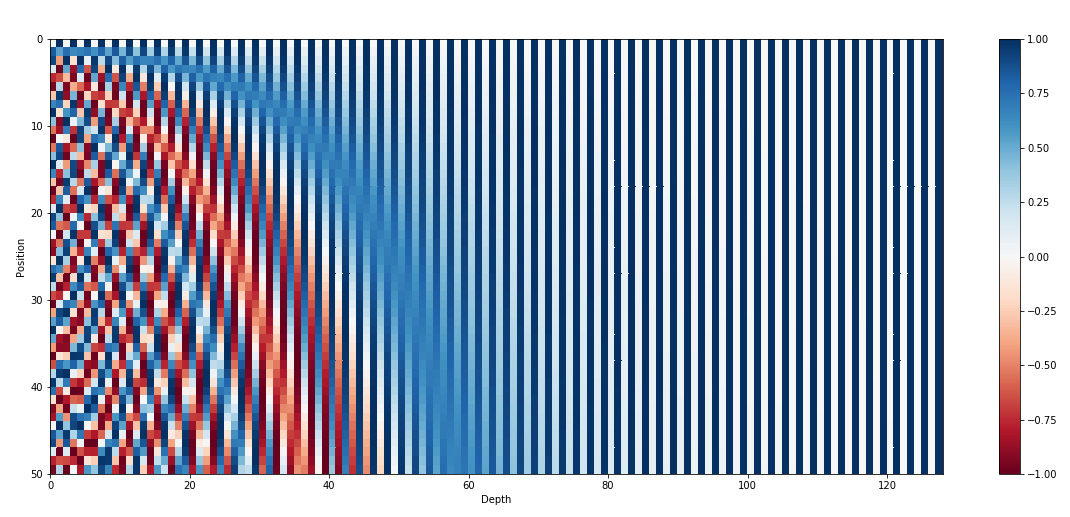
\includegraphics[scale=0.40]{images/positional_encoding.png}
    \centering
    \caption{Position encoding 128 chiều cho một câu có độ dài tối đa là 50}
    \label{position_encoding}
\end{figure}

\subsection{LayoutXLM}
LayoutXLM \cite{xu2021layoutxlm}, một mô hình đã được pre-trained đa phương thức để hiểu văn bản trong nhiều ngôn ngữ khác nhau. Mục tiêu chính của mô hình này là vượt qua rào cản ngôn ngữ trong việc hiểu các văn bản có chứa thông tin hình ảnh đa dạng. Điều độc đáo của LayoutXLM nằm ở việc nó kết hợp thông tin từ văn bản, cấu trúc bố cục và cả hình ảnh để huấn luyện một mô hình Transformer để hiểu tài liệu.

Mô hình đã được huấn luyện bằng cách sử dụng 30 triệu tài liệu số từ 53 ngôn ngữ khác nhau. Kết quả thể hiện rằng LayoutXLM vượt trội hơn so với các mô hình đa ngôn ngữ khác khi được đánh giá trên bộ dữ liệu hiểu biểu mẫu XFUND trong 7 ngôn ngữ khác nhau.

Tóm lại, đây thực sự là một bước đột phá trong nghiên cứu về việc huấn luyện mô hình đa phương tiện và đa ngôn ngữ để hiểu các tài liệu phức tạp chứa cả hình ảnh.

\begin{figure}[h]
    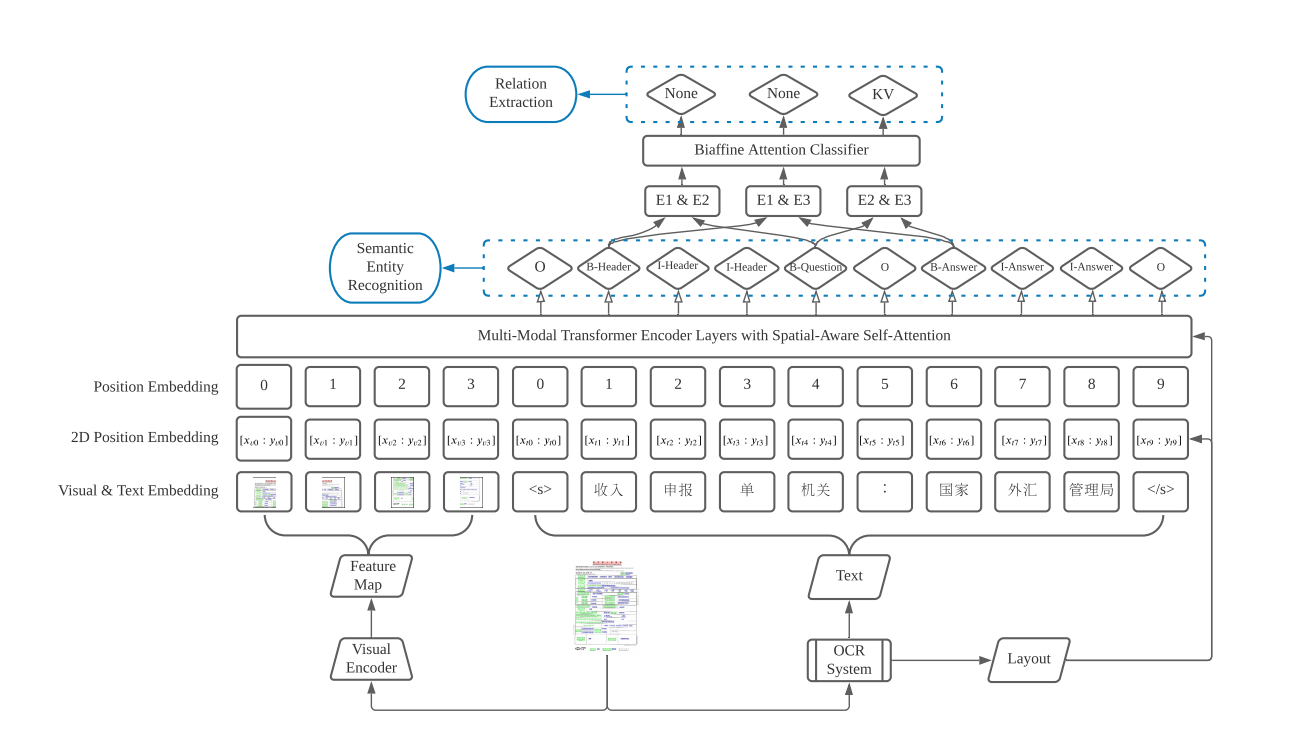
\includegraphics[scale=0.42]{images/layoutxml-architecture.png}
    \caption{Kiến trúc của mô hình LayoutXLM}
    \label{layoutxml}
\end{figure}

Mô hình LayoutXLM được xây dựng với một kiến trúc Transformer đa phương tiện. Kiến trúc được thể hiện trong Hình \ref{layoutxml}. Mô hình chấp nhận thông tin từ ba phương thức khác nhau, bao gồm văn bản, bố cục và hình ảnh, được mã hóa lần lượt bằng các lớp nhúng văn bản, nhúng bố cục và nhúng hình ảnh. Các nhúng văn bản và hình ảnh được nối lại, sau đó cộng với nhúng bố cục để thu được nhúng đầu vào. Những nhúng đầu vào được mã hóa bởi một Transformer đa phương tiện với cơ chế tự-chú ý có thông tin vị trí. Cuối cùng, biểu diễn ngữ cảnh đầu ra có thể được sử dụng cho các lớp cụ thể cho các nhiệm vụ tiếp theo. 

\subsubsection{Kiến trúc mô hình}
\paragraph*{Text Embedding}
Tuân theo thực tiện thông thường, mô hình sử dụng WordPiece để tách thành các từ trong dãy văn bản từ OCR và gán mỗi từ vào một phân đoạn cụ thể $s_i \in \{\mathtt{[A]}, \mathtt{[B]}\}$. Sau đó, thêm $\mathtt{[CLS]}$ ở đầu của dãy và $\mathtt{[SEP]}$ ở cuối mỗi phân đoạn văn bản. Các $\mathtt{[PAD]}$ bổ sung được đặt ở cuối để đảm bảo độ dài cuối cùng của chuỗi chính xác là độ dài tối đa của chuỗi $L$. Nhúng văn bản cuối cùng là tổng của ba embedding. Token embedding đại diện cho chính token, position embedding 1D đại diện cho chỉ số của token, và embedding phân đoạn được sử dụng để phân biệt các phân đoạn văn bản khác nhau. Một cách chính xác hơn, mô hình có text embedding thứ $i$ $(0 \leq i < L)$ như sau \cite{xu2022layoutlmv2}:
\[
    \mathbf{t}_i = \text{TokEmb}(w_i) + \text{PosEmb1D}(i) + \text{SegEmb}(s_i)
\]

\paragraph*{Visual Embedding}
Do mô hình gặp khó khăn trong việc bắt kịp các chi tiết trong hình ảnh toàn bộ trang, nên cần chuyển đổi hình ảnh thành chuỗi có độ dài cố định bằng cách sử dụng bản đồ đặc trưng của mã hóa hình ảnh CNN. Mô hình dùng kiến trúc ResNeXt-FPN làm nền tảng mã hóa hình ảnh. Hình ảnh được chuẩn hóa kích thước và đưa vào mã hóa. Bản đồ đặc trưng đầu ra được làm phẳng thành chuỗi embedding hình ảnh. Một lớp chiếu áp dụng cho mỗi embedding để đồng nhất kích thước với text embedding. Thêm position embedding 1D để bổ sung thông tin vị trí. Tất cả embedding hình ảnh gán vào phân đoạn hình ảnh.

Cho một hình ảnh trang tài liệu $I$, nó được điều chỉnh kích thước thành $224 \times 224$ rồi được đưa vào bộ mã hóa hình ảnh. Sau đó, bản đồ đặc trưng đầu ra lấy trung bình để có kích thước cố định với chiều rộng là $W$ và chiều cao là $H$. Tiếp theo, nó được làm phẳng thành một chuỗi embedding hình ảnh có độ dài là $W \times H$. Chuỗi này được gọi là VisTokEmb($I$). Một lớp chiếu tuyến tính được áp dụng cho mỗi token embedding hình ảnh để đồng nhất kích thước chiều với text embedding. Vì bộ mã hóa hình ảnh dựa trên CNN không thể bắt được thông tin vị trí, chúng tôi cũng thêm position embedding 1D vào các token embedding hình ảnh này. position embedding 1D được sử dụng chung với lớp text embedding. Đối với embedding phân đoạn, chúng tôi gán tất cả các token embedding hình ảnh vào phân đoạn hình ảnh $\mathtt{[C]}$.
embedding hình ảnh thứ $i$ $(0 \leq i < W H)$ có thể được biểu diễn như sau \cite{xu2022layoutlmv2}:
\[
    \mathbf{v}_i = \text{Proj}(\text{VisTokEmb}(I)_i) + \text{PosEmb1D}(i) + \text{SegEmb}([\mathtt{C}])    
\]

\paragraph*{Layout Embedding}
Lớp Layout Embedding dùng để nhúng thông tin bố cục không gian được biểu diễn bởi các khung chữ nhật của các token từ kết quả OCR, trong đó chiều rộng, chiều cao khung cùng với tọa độ góc được xác định. Tất cả các tọa độ được chuẩn hóa và định lượng thành các số nguyên trong khoảng [0, 1000], và sử dụng 2 lớp embedding riêng biệt để nhúng các đặc trưng trục $x$ và trục $y$. Với hộp giới hạn chuẩn hóa của token văn bản/thị giác thứ $i$ $(0 \leq i < W H + L)$ là $\text{box}_i = (x_{min}, x_{max}, y_{min}, y_{max}, width, height)$, lớp layout embedding nối tất cả 6 đặc trưng của hộp giới hạn thành một vector position embedding 2D ở cấp độ token \cite{xu2022layoutlmv2}.
\[
    \mathbf{l}_i = \text{Concat}(\text{PosEmb2D}_\text{x}(x_{\text{min}}, x_{\text{max}}, width), \text{PosEmb2D}_{\text{y}}(y_{\text{min}}, y_{\text{max}}, height))
\]
Như vậy, lớp nhúng bố cục dùng để mã hóa thông tin vị trí không gian của các token dựa trên kết quả OCR thành các vector nhúng, giúp mô hình hiểu được mối quan hệ không gian giữa các token.

\paragraph*{Multi-modal Encoder with Spatial-Aware Self-Attention Mechanism}
Bộ mã hóa kết hợp nhúng hình ảnh và văn bản thành một chuỗi đơn, tích hợp thông tin không gian thông qua nhúng bố cục. Bộ mã hóa hoạt động giống như kiến trúc Transformer, sử dụng nhiều lớp tự chú ý liên tiếp tiếp theo bởi các mạng tiến thẳng. Để giải quyết việc hiểu quả việc nắm bắt mối quan hệ cục bộ trong bố cục tài liệu, một cơ chế tự chú ý nhận thức vị trí được giới thiệu. Khác với tự chú ý ban đầu, phụ thuộc vào thông tin vị trí tuyệt đối, tự chú ý nhận thức vị trí xem xét thông tin vị trí tương đối một cách rõ ràng. Cơ chế này liên quan đến một đầu vào duy nhất trong một lớp tự chú ý, với kích thước ẩn $d_{head}$ và các ma trận chiếu $WQ$, $WK$, và $WV$. Điểm chú ý giữa truy vấn $xi$ và khóa $xj$ được tính toán bằng quá trình chiếu và chuẩn hóa.
\[
    \alpha_{ij} = \frac{1}{\sqrt{d_{head}}}(\mathbf{x}_i \mathbf{W}^Q) (\mathbf{x}_j \mathbf{W}^K)^T
\]

Xem xét khoảng cách rộng lớn của các vị trí, mô hình hóa vị trí tương quan ngữ nghĩa và vị trí tương quan không gian dưới dạng các thành phần bias để ngăn việc thêm quá nhiều tham số. Thực hành tương tự đã được chứng minh hiệu quả trong các kiến trúc Transformer chỉ có văn bản \cite{vaswani2023attention}. Giả sử $\mathbf{b}^{(1D)}$, $\mathbf{b}^{(2D_x)}$ và $\mathbf{b}^{(2D_y)}$ là các bias vị trí tương quan 1D và 2D có thể học được tương ứng. Các bias này khác nhau giữa các đầu chú ý nhưng được chia sẻ trong tất cả các lớp mã hóa. Giả sử $(x_i, y_i)$ là tọa độ góc trên bên trái của hộp giới hạn thứ $i$, chúng ta thu được điểm chú ý nhận thức vị trí không gian như sau:
\[
    \alpha'_{ij} = \alpha_{ij} + \mathbf{b}_{j-i}^{(1\text{D})} + \mathbf{b}_{x_j-x_i}^{(2\text{D}_x)} + \mathbf{b}_{y_j-y_i}^{(2\text{D}_y)}
\]

Cuối cùng, các vector đầu ra được biểu diễn dưới dạng trung bình có trọng số của tất cả các vector giá trị đã được chiếu tương ứng với các điểm chú ý nhận thức vị trí không gian đã được chuẩn hóa \cite{xu2022layoutlmv2}.

\[
    \mathbf{h}_i = \sum_j \frac{\exp(\alpha'_{ij})}{\sum_k \exp(\alpha'_{ik})} \mathbf{x}_j \mathbf{W}^V    
\]

\subsubsection{Nhiệm vụ tiền huấn luyện}
\paragraph*{Masked Visual-Language Modeling}
Masked Visual-Language Modeling giúp mô hình học tốt hơn trong phần ngôn ngữ với các dấu vết chéo-modality. Mô hình ngẫu nhiên che đi một số token văn bản và yêu cầu mô hình phục hồi các token bị che. Trong khi đó, thông tin về bố cục vẫn không thay đổi, điều này có nghĩa là mô hình biết vị trí của từng mã thông báo bị che trên trang. Các biểu diễn đầu ra của các token bị che từ bộ mã hóa được đưa vào một bộ phân loại trên toàn bộ từ vựng, dựa trên một mất mát cross-entropy. Để tránh rò rỉ dấu vết hình ảnh, Mô hình che khu vực hình ảnh tương ứng với các token bị che trên đầu vào hình ảnh trang gốc trước khi đưa nó vào bộ mã hóa hình ảnh.

\paragraph*{Text-Image Alignment}
Để giúp mô hình học được sự tương ứng vị trí không gian giữa hình ảnh và tọa độ của các hộp giới hạn, Mô hình đề xuất Nhiệm vụ \acrfull*{tia} như một nhiệm vụ căn chỉnh chéo chi tiết hơn. Trong nhiệm vụ \acrshort*{tia}, một số dòng văn bản được chọn ngẫu nhiên và các khu vực hình ảnh tương ứng của chúng được che trên hình ảnh tài liệu. Thao tác này được gọi là ``covering'' để tránh sự nhầm lẫn với thao tác ``masking'' trong \acrshort*{mvlm}. Trong quá trình tiền huấn luyện, một lớp phân loại được xây dựng trên đầu ra của bộ mã hóa. Lớp này dự đoán một nhãn cho mỗi mã thông báo văn bản tùy thuộc vào việc nó được che, tức là [\texttt{Covered}] hoặc [\texttt{Not Covered}], và tính mất mát nhị phân cross-entropy. Xem xét độ phân giải của hình ảnh đầu vào có hạn, và một số yếu tố trong tài liệu như biển báo và thanh trong một hình ảnh có thể giống như các vùng văn bản bị che, nhiệm vụ tìm kiếm một vùng hình ảnh bị che cỡ từ có thể gây nhiễu. Do đó, thao tác che được thực hiện ở mức dòng văn bản. Khi \acrshort*{mvlm} và \acrshort*{tia} được thực hiện đồng thời, các mất mát \acrshort*{tia} của các mã thông báo bị che trong \acrshort*{mvlm} không được tính vào. Điều này ngăn mô hình học được sự tương ứng không hữu ích nhưng trực tiếp từ [\texttt{MASK}] đến [\texttt{Covered}].

\paragraph*{Text-Image Matching}
Hơn nữa, một nhiệm vụ căn chỉnh chéo chi tiết hơn, Nhiệm vụ \acrfull*{tim}, được áp dụng để giúp mô hình học sự tương ứng giữa hình ảnh tài liệu và nội dung văn bản. Chúng tôi đưa biểu diễn đầu ra tại [\texttt{CLS}] vào một bộ phân loại để dự đoán xem hình ảnh và văn bản có đến từ cùng một trang tài liệu hay không. Các đầu vào thông thường được sử dụng là các mẫu tích cực. Để xây dựng một mẫu tiêu cực, một hình ảnh có thể được thay thế bằng một hình ảnh trang từ tài liệu khác hoặc bị bỏ qua. Để ngăn mô hình gian lận bằng cách tìm các đặc trưng của nhiệm vụ, chúng tôi thực hiện các thao tác masking và covering tương tự cho các hình ảnh trong các mẫu tiêu cực. Nhãn mục tiêu \acrshort*{tim} trong các mẫu tiêu cực được thiết lập là [\texttt{Covered}] cho tất cả. Chúng tôi áp dụng mất mát nhị phân cross-entropy trong quá trình tối ưu hóa.

\subsection{DBNet}
\acrfull*{dbnet} \cite{liao2019realtime}, đây là một mô hình mạng nơ-ron sử dụng trong lĩnh vực phát hiện văn bản. Phương pháp này tập trung vào vấn đề chuyển đổi hình ảnh văn bản đa dạng thành hình ảnh nhị phân, đồng thời huấn luyện mạng theo cách có thể tối ưu hóa quá trình này. Phương pháp nhị phân hoá khác biệt của DBNet cho phép giữ lại thông tin quan trọng trong hình ảnh và loại bỏ thông tin không cần thiết, giúp cải thiện độ chính xác của quá trình nhận dạng ký tự.

DB là một thuật toán dựa trên phân đoạn để phát hiện văn bản, sử dụng một mô-đun Nhị phân hóa Ngưỡng Khả vi (DB) khác biệt để phân biệt vùng văn bản khỏi nền với một ngưỡng động.

\begin{figure}[h]
    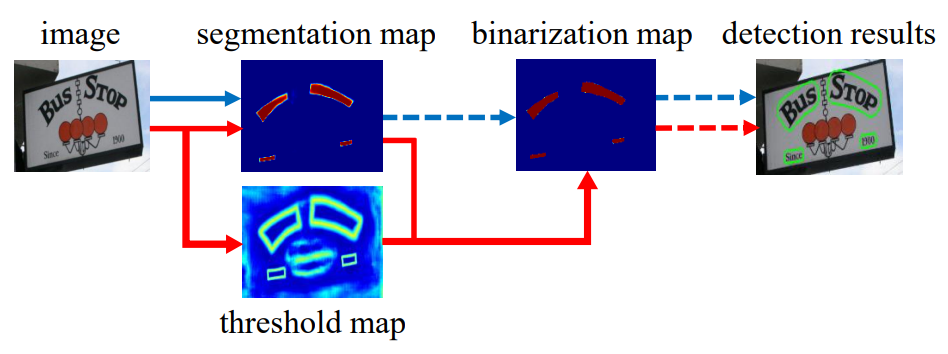
\includegraphics[scale=0.5]{images/tradition-db-pipeline.png}
    \centering
    \caption{Pipeline truyền thống (luồng màu xanh) và pipeline của DB (luồng màu đỏ) }
    \label{}
\end{figure}

Những mũi tên màu xanh trong hình minh họa cho quy trình của các thuật toán phát hiện văn bản dựa trên phân đoạn thông thường. Loại phương pháp này sử dụng một ngưỡng cố định để tạo ra bản đồ phân đoạn nhị phân sau khi phân đoạn, sau đó áp dụng các thuật toán heuristics như gom cụm pixel để có được vùng văn bản.
Những mũi tên màu đỏ trong hình minh họa cho luồng của thuật toán DB. Sự khác biệt lớn nhất so với các giải pháp thông thường là DB có một bản đồ ngưỡng, và nó sẽ dự đoán ngưỡng tại mỗi điểm pixel của hình ảnh thông qua mạng neural, thay vì chỉ định một giá trị cố định. Do đó, nó có thể phân biệt tốt hơn giữa nền và vùng văn bản.

Thuật toán DB có những ưu điểm sau:
\begin{enumerate}
    \item Cấu trúc thuật toán đơn giản và không cần xử lý sau quá trình tính toán phức tạp
    \item Dữ liệu nguồn mở của nó có độ chính xác và hiệu suất tốt
\end{enumerate}
Sau khi có bản đồ xác suất, thuật toán truyền thống dựa trên phân đoạn hình ảnh sẽ đặt tất cả các điểm ảnh có giá trị thấp hơn ngưỡng t thành 0 và ngược lại thành 1. Công thức là: 
$$
B_{i, j} = \begin{cases}
    1, \text{if } P_{i, j} \geq t, \\
    0, \text{otherwise}
\end{cases} 
$$

Nhưng phương pháp nhị phân tiêu chuẩn không có khả năng khác biệt, từ đó khiến mạng không thể được huấn luyện theo kiểu end-to-end (tức là không thể tích hợp vào quá trình lan truyền ngược). Để giải quyết vấn đề này, thuật toán DB sử dụng Differentiable Binarization, giúp xấp xỉ step function của phương pháp nhị phân tiêu chuẩn. Nó sử dụng công thức khác:
\[
    \hat{B} = \frac{1}{1+e^{-k(P_{i, j} - T_{i, j})}}    
\]

Ở trên, $P$ đề cập đến bản đồ xác suất, $T$ đề cập đến bản đồ ngưỡng, và $k$ là hệ số tăng được thiết lập là 50 dưới một quy tắc thực tế trong thí nghiệm. Hình \ref{fig11}(a) dưới đây cho thấy sự khác biệt giữa phương pháp nhị phân tiêu chuẩn và phân đoạn khác biệt.

Khi sử dụng hàm mất mát cross-entropy, mất mát của các mẫu dương và mẫu âm lần lượt là $l_+$ và $l_-$:
\[
    l_+ = -\log(\frac{1}{1+e^{-k(P_{i, j}-T_{i, j})}})
\]
\[
    l_- = -\log(1 - \frac{1}{1 + e^{-k(P_{i, j} - T_{i, j})}})
\]

Nhập $x$ vào để lấy đạo hàm riêng có thể dẫn đến:
\[
    \frac{\delta l_+}{\delta x} = -kf(x)e^{-kx}
\]
\[
    \frac{\delta l_-}{\delta x} = -kf(x)   
\]

Có thể thấy rằng hệ số tăng sẽ làm phình to độ dốc của dự đoán lỗi, từ đó tối ưu hóa mô hình để đạt được kết quả tốt hơn. Trong Hình \ref{fig11}(b), phần của $x < 0$ đại diện cho trường hợp mẫu tích cực được dự đoán thành mẫu tiêu cực. Có thể thấy rằng hệ số tăng k làm phình to độ dốc. Hình \ref{fig11}(c) hiển thị $x > 0$, đề cập đến trường hợp mẫu tiêu cực được dự đoán thành mẫu tích cực, và độ dốc cũng được phình to.

\begin{figure}[h]
    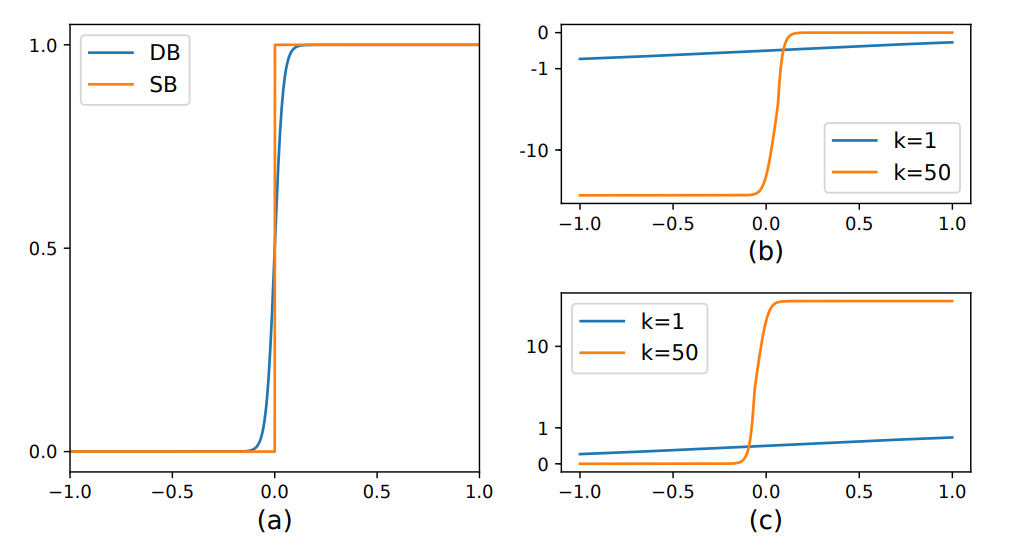
\includegraphics[scale=0.5]{images/derivative-DB.png}
    \centering
    \caption{Minh họa về phân đoạn khác biệt và đạo hàm của nó. (a) So sánh số liệu giữa phương pháp nhị phân tiêu chuẩn (SB) và phân đoạn khác biệt (DB). (b) Đạo hàm của $l_+$. (c) Đạo hàm của $l_-$. \cite{liao2019realtime}}
    \label{fig11}
\end{figure}

\begin{figure}[h]
    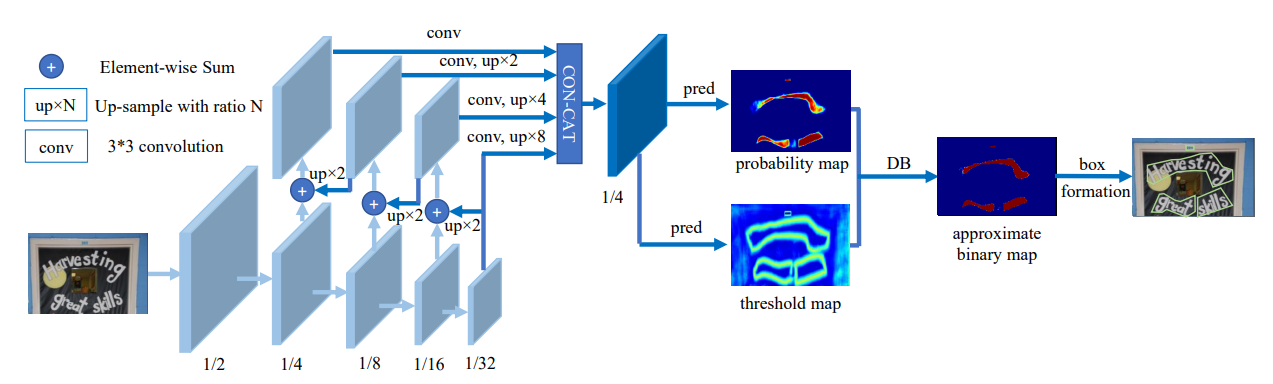
\includegraphics[scale=0.45]{images/architecture-db.png}
    \centering
    \caption{Kiến trúc của phương pháp DB}
    \label{fig12}
\end{figure}

Cấu trúc tổng quan của thuật toán DB (Hình \ref{fig12}), các đặc điểm của hình ảnh đầu vào được trích xuất thông qua mạng Backbone và FPN, sau đó chúng được nối liền để tạo ra một đặc điểm có kích thước là một phần tư của hình ảnh gốc. Sau đó, lớp tích chập được sử dụng để tạo ra bản đồ xác suất dự đoán và bản đồ ngưỡng, và sau đó tạo ra đường viền qua quá trình xử lý sau cùng của DB.

\subsection{TransformerOCR}
Để nhận dạng văn bản bằng tiếng việt, em sử dụng mã nguồn mở VietOCR đây là một mô hình được cài đặt trên Transformer OCR. Dùng để nhận dạng chữ viết tay, chữ đánh máy cho Tiếng Việt.

\begin{figure}[h]
    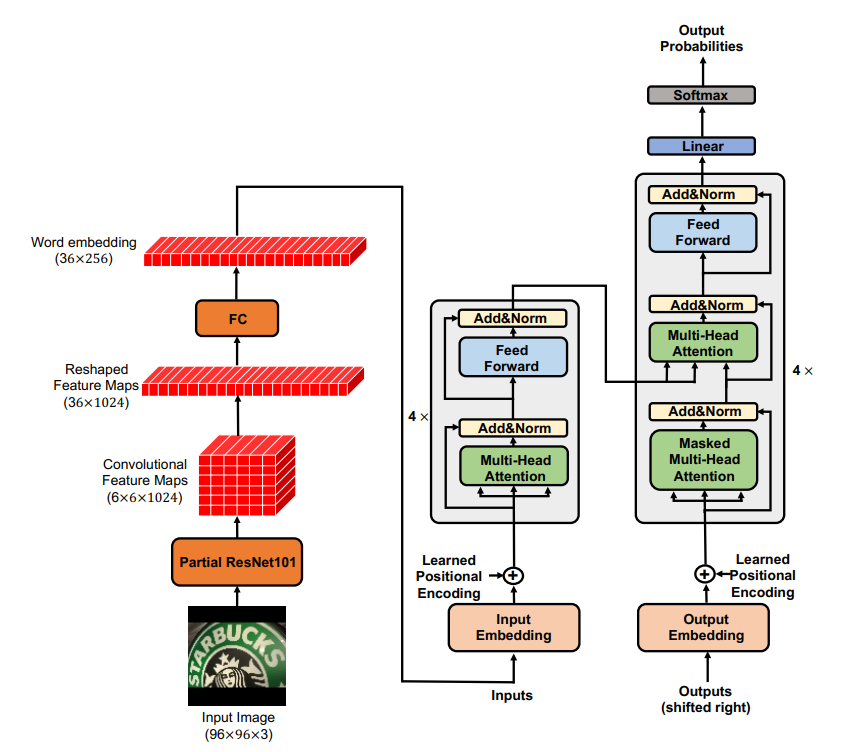
\includegraphics[scale=0.65]{images/overview-transOCR.png}
    \centering
    \caption{Kiến trúc tổng qua của TransformerOCR \cite{feng2020scene}}
    \label{overview-transOCR}
\end{figure}

TransformerOCR là một sự kết hợp tuyệt vời giữa mô hình CNN và Transformer Hình \ref{overview-transOCR}, được áp dụng rộng rãi trong lĩnh vực nhận dạng ký tự quang học. Mô hình bao gồm hai mô-đun chính: mô-đun trích xuất đặc trưng và mô-đun transformer. Mô-đun trích xuất đặc trưng được sử dụng ban đầu để tạo ra các bản đồ đặc trưng từ một hình ảnh đầu vào. Sau đó, các bản đồ đặc trưng được đưa vào mô-đun transformer như là nhúng từ đầu vào.

\subsubsection*{Mô-đun Trích xuất đặc trưng}
Có rất nhiều mạng \acrshort*{cnn} có thể được sử dụng để trích xuất đặc trưng. Mô hình \acrshort*{cnn} dùng trong bài toán \acrshort*{ocr} nhận đầu vào là một ảnh, thông thường có kích thước với chiều dài lớn hơn nhiều so với chiều rộng, do đó việc điều chỉnh tham số stride size của tầng pooling là cực kì quan trọng. Việc chọn kích thước stride size của các lớp pooling cuối cùng là $w \times x = 2 \times 1$ trong mô hình OCR. Không thay đổi stride size phù hợp với kích thước ảnh thì sẽ dẫn đến kết quả nhận dạng của mô hình sẽ tệ.

Đối với mô hình VGG, việc thay đổi pooling size khá dễ do kiến trúc đơn giản, tuy nhiên đối với mô hình phức tạp khác như resnet việc điều chỉnh tham số pooling size hơi phức tạp do một ảnh bị downsampling không chỉ bởi tầng pooling mà còn tại các tầng convolution khác.

Một ảnh qua mô hình CNN, sẽ cho một feature maps có kích thước (width $\times$ height) $\times$ batch $\times$ channels, feature maps này sẽ trở thành đầu vào cho mô hình Transformer.

\subsubsection*{Mô-đun Transformer}
Transformer là một mô hình cách mạng trong xử lý ngôn ngữ tự nhiên. Nhờ cơ chế attention mạnh mẽ, transformer vượt trội hơn đáng kể so với hầu hết các mô hình attention dựa trên RNN. Khác với local attention dựa trên RNN, transformer có phạm vi global attention. Như được minh họa trong Hình \ref{overview-transOCR}, transformer có cấu trúc mã hóa-giải mã. Bộ mã hóa ánh xạ các bản đồ đặc trưng $(x_1, ..., x_{n})$ do mô-đun trích xuất đặc trưng tạo ra thành một chuỗi các biểu diễn liên tục $z = (z_1, ..., z_{n})$. Dựa trên $z$, bộ giải mã sau đó tạo ra một chuỗi đầu ra $(y_1, ..., y_m)$ của các ký hiệu một phần tử tại một thời điểm. Ở mỗi bước, mô hình là tự hồi quy, tiêu thụ các ký hiệu được tạo ra trước đó như đầu vào bổ sung khi tạo ra ký hiệu tiếp theo \cite{feng2020scene}.

Trong mô hình này, hình ảnh đầu vào có góc nhìn hai chiều. Do đó, mã hóa vị trí cố định một chiều không phù hợp. Thay vào đó, mô hình sử dụng nhúng vị trí có thể học được trong mô hình đề xuất. Nhờ cơ chế Attention mạnh mẽ của transformer, mô hình thực hiện lưu giữ đầu ra CNN dưới dạng Spatial attention. Tại mỗi bước giải mã, một mô-đun Attention nhìn thấy spatial attention. Bằng cách này, mô hình đạt được hiệu suất tốt nhất trên các bộ dữ liệu nhận dạng văn bản không đều và kết quả có thể so sánh trên các tập dữ liệu văn bản thông thường

Tại sao không sử dụng các mô hình chú ý dựa trên RNN? Lý do chính là, RNN xử lý chuỗi đầu vào một cách tuần tự, cơ chế này khiến cho RNN có xu hướng thu thập thông tin cục bộ hơn. Cái tồi tệ hơn là RNN không có khả năng bù đắp cho sự mất mát thông tin không gian khi chuyển đổi bản đồ đặc trưng hai chiều thành một chiều. Nhưng transformer xử lý chuỗi đầu vào theo cách song song, mỗi đặc trưng đơn lẻ có thể có tất cả sự chú ý từ đầu vào. Mặc dù việc sắp xếp lại bản đồ đặc trưng từ hai chiều thành một chiều sẽ mất thông tin không gian, mã hóa vị trí học được có khả năng bù đắp cho sự mất mát này \cite{feng2020scene}.

\subsection{Ứng dụng trong OCR}
Học sâu đã được chứng minh là có hiệu quả hơn các phương pháp OCR truyền thống \cite{ai-vs-traditional}, đặc biệt là đối với các tài liệu có chất lượng thấp hoặc bị định dạng phức tạp.

Một số ứng dụng của Học sâu trong OCR bao gồm:
\begin{itemize}
    \item Nhận dạng hóa đơn: Học sâu có thể được sử dụng để nhận dạng các trường thông tin quan trọng trên hóa đơn, chẳng hạn như tên người mua, người bán, ngày giao dịch, số lượng, giá và tổng số tiền. Điều này có thể giúp tiết kiệm thời gian và chi phí cho các doanh nghiệp, đồng thời cải thiện độ chính xác của việc xử lý hóa đơn.
    \item Nhận dạng tài liệu y tế: Học sâu có thể được sử dụng để nhận dạng thông tin quan trọng trên tài liệu y tế, chẳng hạn như tên bệnh nhân, chẩn đoán, phương pháp điều trị và các loại thuốc được kê đơn. Điều này có thể giúp cải thiện chất lượng chăm sóc bệnh nhân và giảm chi phí chăm sóc sức khỏe.
    \item Nhận dạng tài liệu pháp lý: Học sâu có thể được sử dụng để nhận dạng thông tin quan trọng trên tài liệu pháp lý, chẳng hạn như tên các bên liên quan, ngày tháng, các điều khoản của thỏa thuận và các điều khoản của hợp đồng. Điều này có thể giúp các luật sư và chuyên gia pháp lý tìm kiếm thông tin nhanh chóng và dễ dàng hơn.
    \item Nhận dạng tài liệu tài chính: Học sâu có thể được sử dụng để nhận dạng thông tin quan trọng trên tài liệu tài chính, chẳng hạn như tên công ty, giá cổ phiếu, số lượng cổ phiếu và giá trị thị trường của cổ phiếu. Điều này có thể giúp các nhà đầu tư và các chuyên gia tài chính đưa ra quyết định đầu tư tốt hơn.
\end{itemize}
Học sâu là một công nghệ mạnh mẽ có thể được sử dụng để cải thiện độ chính xác và hiệu quả của OCR. Với sự phát triển của Học sâu, OCR sẽ trở nên dễ dàng và thuận tiện hơn trong tương lai.

Chương này em đã mô tả các lý thuyết liên quan đến OCR, học sâu và các thuật toán, phương pháp nổi bật của từng nhiệm vụ riêng lẻ. Trong chương tiếp theo em sẽ giới thiệu về các công cụ và thư viện cần thiết.

% Chương 3 ======================================================================
\newpage
\chapter{Công cụ và môi trường thực hiện}
Trong trương này em sẽ trình bày những công cụ và môi trường cần thiết trong quá trình huấn luyện mô hình \acrshort*{ocr}. Dưới đây là các bước trình bày chi tiết:
\begin{enumerate}
    \item \textbf{Phầm mềm và công cụ hỗ trợ:} Trình bày các phầm mềm và công cụ cho quá trình chuẩn bị dữ liệu, huấn luyện và xây dựng mô hình.
    \item \textbf{Tạo môi trường và cài công cụ cần thiết}: Trình bày các bước cài đặt môi trường cho đề tài và thiết lập một số môi trường cần thiết để chạy.

\end{enumerate}

Các công cụ và môi trường là nền tảng quan trọng cho việc thực hiện nghiên cứu, giúp định hình cách tiến hành các bước quan trọng trong đề tài ``Nghiên cứu ứng dụng công nghệ OCR nhận dạng hóa đơn''.

\section{Phầm mềm và công cụ hỗ trợ}
\subsection{Google Colab}
Google Colab (viết tắt của Google Colaboratory) là một dịch vụ miễn phí của Google cho phép thực hiện và chia sẻ các tệp notebook Jupyter, cũng như code Python. Nó là một môi trường trực tuyến, cho phép người dùng viết và chạy code Python một cách trực tiếp trên trình duyệt web mà không cần cài đặt bất kỳ môi trường phát triển nào trên máy tính.

Colab cung cấp sử dụng miễn phí cho CPU, GPU và RAM để người dùng có thể thực hiện các nhiệm vụ tính toán phức tạp mà không cần phải mua hoặc cấu hình phần cứng riêng. Colab còn được tích hợp sẵn với nhiều thư viện phổ biến cho khoa học dữ liệu, học máy và xử lý ảnh, giúp dễ dàng tiến hành các tác vụ phức tạp. Có thể tạo notebook Jupyter, trong đó bạn có thể viết code Python từng cell và thực thi chúng một cách tương tác. Điều này rất hữu ích cho việc thử nghiệm, phân tích dữ liệu và xây dựng mô hình máy học.

Colab có thể chia sẻ notebook của mình với người khác thông qua liên kết. Người khác có thể xem và chỉnh sửa notebook hoặc thậm chí làm việc chung với nhau trên cùng một notebook. Có thể lưu notebook và dữ liệu của mình trực tiếp vào Google Drive để truy cập dễ dàng và chia sẻ với các thiết bị khác.

Google Colab thường được sử dụng trong việc học, nghiên cứu và phát triển các dự án liên quan đến khoa học dữ liệu, học máy và trí tuệ nhân tạo mà không cần đầu tư nhiều vào cấu hình phần cứng.

\subsection{Vast.ai}
Vast.ai là một nền tảng tính toán phi tập trung cho phép bất cứ ai cho thuê công suất tính toán dư thừa của mình để kiếm tiền. Nó kết nối những người cần công suất tính toán bổ sung cho các tác vụ như học máy với những người có GPU hoặc CPU nhàn rỗi trên máy tính của họ. Một số tính năng chính của Vast.ai:

\begin{itemize}
    \item Mạng phi tập trung: Vast.ai chạy trên mạng ngang hàng phi tập trung thay vì máy chủ tập trung. Điều này làm cho nó bền vững và minh bạch hơn.
    \item Cho thuê công suất tính toán dư thừa: Mọi người có thể cài đặt ứng dụng khách Vast.ai trên máy tính của họ để cho thuê bất kỳ chu kỳ GPU hoặc CPU không sử dụng nào và được trả bằng tiền điện tử. Điều này cho phép mọi người kiếm tiền từ các tài nguyên tính toán dư thừa.
    \item Thuê công suất tính toán: Các nhà nghiên cứu, nhà phát triển và những người khác cần công suất tính toán bổ sung cho các ứng dụng như huấn luyện học máy có thể thuê GPU và CPU theo yêu cầu thông qua sàn giao dịch vast.ai. Giá được định giá động dựa trên cung và cầu.
    \item Mã nguồn mở: Vast.ai là một dự án nguồn mở được xây dựng trên các công nghệ phi tập trung hiện có. Điều này cho phép tính minh bạch và đóng góp của cộng đồng vào nền tảng.
\end{itemize}
Vast.ai tạo ra mô hình kinh tế chia sẻ cho công suất tính toán, kết nối những người có nguồn lực dư thừa với những người cần chúng theo cách ngang hàng phi tập trung. Nó cung cấp một cách dễ dàng để bất cứ ai có thể kiếm tiền từ công suất tính toán không sử dụng.

\subsection{CUDA Toolkit}
CUDA Toolkit (Compute Unified Device Architecture Toolkit) là một bộ công cụ và thư viện phát triển bởi NVIDIA dành cho việc phát triển ứng dụng và tính toán sử dụng các GPU của NVIDIA. CUDA là một mô hình lập trình và nền tảng tích hợp vào GPU để thực hiện tính toán đồng thời và xử lý dữ liệu song song. Điều này cho phép các ứng dụng thực hiện tính toán nhanh hơn trên GPU so với việc sử dụng CPU truyền thống.

CUDA Toolkit bao gồm các thành phần quan trọng sau đây:
\begin{enumerate}
    \item \textbf{CUDA Runtime}: CUDA Runtime là một tập hợp các thư viện và API cho phép ứng dụng tương tác với GPU và thực hiện các phép tính trên GPU. Nó cho phép bạn chạy các chương trình CUDA trên GPU của NVIDIA.
    \item \textbf{CUDA Compiler}: CUDA Toolkit đi kèm với trình biên dịch nvcc để biên dịch mã CUDA C/C++ thành mã máy GPU thực thi được.
    \item \textbf{CUDA Libraries}: CUDA Toolkit cung cấp một loạt thư viện cho các loại tính toán khác nhau, bao gồm thư viện đại số tuyến tính, thư viện xử lý ảnh, thư viện tính toán máy học (cuDNN, cuBLAS), và nhiều thư viện khác.
    \item \textbf{CUDA SDK}: CUDA SDK cung cấp các ví dụ và tài liệu hướng dẫn để bạn có thể bắt đầu phát triển ứng dụng sử dụng CUDA.
    \item \textbf{NVIDIA GPU Driver}: CUDA Toolkit yêu cầu cài đặt đúng phiên bản driver cho GPU của bạn để hoạt động.
\end{enumerate}

CUDA Toolkit thường được sử dụng trong lĩnh vực deep learning, scientific computing, và các ứng dụng đòi hỏi tính toán song song và xử lý số lớn. Nó cho phép các nhà phát triển tận dụng sức mạnh của GPU để gia tăng hiệu suất tính toán và tốc độ xử lý dữ liệu cho các ứng dụng của họ.

\subsection{cuDNN}
Đây là một thư viện phần mềm do NVIDIA phát triển, được tối ưu hóa cho việc thực hiện các phép tính liên quan đến mạng nơ-ron trên GPU. Tên gọi "cuDNN" viết tắt của "CUDA Deep Neural Network library," cho thấy rằng nó được phát triển để hỗ trợ hiệu suất cao khi sử dụng GPU để huấn luyện và triển khai các mô hình mạng nơ-ron sâu (deep neural networks).

Thư viện cung cấp một loạt các chức năng và thư viện tối ưu hóa để thực hiện các phép tính phổ biến trong deep learning, bao gồm các phép tính như: Convolution, Pooling, Normalization, Activation, Recurrent, \ldots

cuDNN được tích hợp vào nhiều framework deep learning phổ biến như TensorFlow và PyTorch, giúp cải thiện hiệu suất huấn luyện và triển khai mô hình trên GPU. Nó đóng vai trò quan trọng trong việc tăng tốc quá trình huấn luyện và triển khai mô hình deep learning trên nền tảng GPU của NVIDIA.
\subsection{PaddleOCR}
PaddleOCR là một dự án mã nguồn mở do PaddlePaddle phát triển, nhằm cung cấp một giải pháp toàn diện cho các nhiệm vụ liên quan đến xử lý ảnh và văn bản, bao gồm cả nhận dạng ký tự, nhận dạng văn bản và các tác vụ liên quan đến OCR. Dự án này được xây dựng trên cơ sở của các mô hình học sâu và sử dụng các thuật toán tiên tiến để giải quyết các thách thức trong việc xử lý ảnh và văn bản.

PaddleOCR hỗ trợ nhiều tác vụ liên quan đến OCR như nhận dạng ký tự, nhận dạng văn bản và phân loại chữ viết tay. Có thể được đào tạo và sử dụng cho nhiều ngôn ngữ khác nhau, giúp phát triển ứng dụng OCR toàn cầu. Người dùng có thể tùy chỉnh và đào tạo lại các mô hình của PaddleOCR cho phù hợp với nhu cầu cụ thể của dự án.

PaddleOCR có thể hoạt động trên nhiều nền tảng khác nhau, bao gồm máy tính cá nhân, máy chủ và các môi trường đám mây. Dự án cung cấp một loạt các mô hình học sâu đã được đào tạo trước để giúp giải quyết các vấn đề liên quan đến xử lý ảnh và văn bản.

Dự án được tối ưu hóa để đạt hiệu suất cao và đáp ứng yêu cầu xử lý ảnh và văn bản trong thời gian thực.

Hơn nữa PaddleOCR là một dự án mã nguồn mở và có cộng đồng hỗ trợ sẵn sàng chia sẻ kiến thức, giải đáp thắc mắc và cùng nhau phát triển.

Tóm lại, cung cấp một giải pháp mạnh mẽ và linh hoạt cho các ứng dụng liên quan đến xử lý ảnh và văn bản, đặc biệt là trong lĩnh vực OCR. Điều này giúp đơn giản hóa và tối ưu hóa quá trình xây dựng hệ thống nhận dạng văn bản và thông tin từ các hình ảnh hóa đơn và tài liệu khác.

\subsection{PPOCRLabel}
PPOCRLabel là một công cụ hỗ trợ trong lĩnh vực xử lý ảnh và trí tuệ nhân tạo, được sử dụng để thực hiện công việc nhận dạng và đánh dấu vùng chứa văn bản trên ảnh. Đây là một dự án mã nguồn mở của PaddlePaddle, một thư viện học máy phát triển bởi Baidu. PaddleOCR nhằm mục tiêu xây dựng các mô hình nhận dạng ký tự trên ảnh với hiệu suất cao.

PPOCRLabel được tạo ra để hỗ trợ quá trình chuẩn bị dữ liệu cho việc huấn luyện mô hình nhận dạng văn bản. Việc chuẩn bị dữ liệu là một bước quan trọng trong quá trình phát triển mô hình học máy, và công cụ như PPOCRLabel giúp đơn giản hóa và tăng cường hiệu suất của quá trình này. Dưới đây là một số tính năng chính của PPOCRLabel \cite{ppocrlabel}:
\begin{enumerate}
    \item \textbf{Labeling vùng chứa văn bản:} PPOCRLabel cho phép người dùng vẽ các hộp giới hạn xung quanh các vùng chứa văn bản trên ảnh để đánh dấu vị trí của văn bản cần nhận dạng.
    \item \textbf{Labeling trích xuất từ khóa:} Người dùng có thể gán nhãn thông tin từ khóa để cho bài toán trích xuất thông tin chính.
    \item \textbf{Gắn nhãn văn bản:} Người dùng có thể gắn nhãn văn bản được nhận dạng trong các hộp giới hạn để cho biết nội dung của văn bản đó.
    \item \textbf{Chú thích cho bảng:} PPOCRLabel cung cấp cho người dùng chức năng chú thích bảng nhằm mục đích bóc tách cấu trúc của bảng dưới dạng hình ảnh và chuyển sang định dạng Excel
    \item \textbf{Chỉnh sửa và xem trước:} PPOCRLabel cung cấp giao diện để chỉnh sửa và xem trước dữ liệu đã được đánh dấu trên ảnh, đảm bảo rằng dữ liệu được chuẩn bị chính xác trước khi sử dụng để huấn luyện mô hình.
    \item \textbf{Xuất dữ liệu:} Sau khi hoàn thành việc đánh dấu và chuẩn bị dữ liệu, PPOCRLabel cho phép bạn xuất dữ liệu trong các định dạng phổ biến để sử dụng trong quá trình huấn luyện mô hình.
    \item \textbf{Tích hợp với PaddleOCR:} PPOCRLabel có thể liên kết với dự án PaddleOCR để tiện lợi trong việc sử dụng dữ liệu đã được chuẩn bị để huấn luyện các mô hình nhận dạng văn bản.
\end{enumerate}

PPOCRLabel là một công cụ cực kỳ hữu ích trong quá trình chuẩn bị dữ liệu cho việc huấn luyện mô hình liên quan đến OCR, giúp tăng cường hiệu suất và chính xác của mô hình cuối cùng.

\subsection{Pytorch}
PyTorch là một thư viện mã nguồn mở được phát triển bởi Facebook's AI Research lab dùng cho việc xây dựng và huấn luyện các mạng nơ-ron. Nó được thiết kế đặc biệt để hỗ trợ tính toán trên mạng nơ-ron và dự án thực tế với sự linh hoạt và hiệu suất cao. PyTorch là một trong những thư viện phổ biến nhất cho deep learning và machine learning trong cộng đồng nghiên cứu và phát triển AI.

Một số điểm mạnh của PyTorch bao gồm:
\begin{enumerate}
    \item Tính năng tạo đồ thị động: PyTorch sử dụng một cơ chế đồ thị tính toán động, cho phép bạn xây dựng và điều chỉnh mô hình một cách linh hoạt trong quá trình chạy. Điều này rất hữu ích khi bạn cần xây dựng các mô hình phức tạp hoặc thực hiện các thay đổi động.
    \item Hỗ trợ GPU: PyTorch có tích hợp sẵn hỗ trợ tính toán trên GPU, giúp gia tăng tốc độ huấn luyện mô hình đáng kể.
    \item Cộng đồng phát triển mạnh mẽ: PyTorch có một cộng đồng người dùng và phát triển đông đảo, nên bạn có thể tìm thấy nhiều tài liệu học tập và hỗ trợ từ cộng đồng.
    \item Sử dụng dễ dàng: PyTorch có một cú pháp Python thân thiện và dễ đọc, giúp người dùng dễ dàng hiểu và sử dụng.
\end{enumerate}
PyTorch cung cấp các thành phần cơ bản để xây dựng và huấn luyện mạng nơ-ron, bao gồm tensor, autograd (tự động tính đạo hàm), và một loạt các lớp và hàm tiện ích để xây dựng mô hình. Nó đã trở thành một trong những công cụ quan trọng cho nghiên cứu và phát triển trong lĩnh vực deep learning.

\subsection{Gradio}
Gradio là một thư viện mã nguồn mở được sử dụng để xây dựng giao diện người dùng cho các mô hình học máy và học sâu một cách dễ dàng và nhanh chóng. Thư viện này giúp tạo ra các ứng dụng web hoặc desktop đơn giản để tương tác với các mô hình đã huấn luyện mà bạn đã xây dựng hoặc sử dụng.

Thư viện cung cấp một API Python dễ sử dụng để bạn có thể định nghĩa các giao diện người dùng tương tác cho các mô hình học máy và học sâu của mình. Với Gradio, ta có thể tạo các biểu đồ, hộp văn bản, nút bấm và các phần tử UI khác để tương tác với mô hình. Gradio cũng hỗ trợ việc hiển thị kết quả và dự đoán từ mô hình trực tiếp trong giao diện người dùng.

Gradio được thiết kế để đơn giản hóa việc tạo giao diện người dùng cho các mô hình học máy mà không cần kiến thức về phát triển web phức tạp. Tương thích với nhiều loại mô hình có thể sử dụng Gradio với các mô hình học máy, deep learning và thậm chí cả các mô hình không cần kết nối mạng. Hỗ trợ cả ứng dụng web và desktop, cho phép triển khai giao diện người dùng trên nhiều nền tảng.

Thư viện có khả năng tích hợp với các framework học máy và deep learning phổ biến như TensorFlow, PyTorch, và Scikit-Learn. Người dùng có thể tùy chỉnh giao diện người dùng của mình bằng cách thêm các phần tử UI và tuỳ chỉnh cách hiển thị kết quả.

Gradio giúp nhanh chóng tạo ra các ứng dụng tương tác cho các mô hình học máy của bạn mà không cần kiến thức chuyên sâu về phát triển giao diện người dùng. Điều này có thể rất hữu ích trong việc trình bày và thử nghiệm các mô hình với người dùng cuối.

\section{Cấu hình phần cứng}
Huấn luyện một mô hình học sâu đòi hỏi xử lý một lượng lớn dữ liệu và tính toán phức tạp. Cần phần cứng mạnh mẽ để xử lý nhanh chóng và hiệu quả. Phần cứng yếu sẽ làm chậm quá trình huấn luyện.Pphần cứng chất lượng cao cho phép huấn luyện nhanh hơn, với dữ liệu lớn hơn và mô hình phức tạp hơn. Do đó với từng tác vụ khác nhau em sẽ xử dụng một cấu hình khác nhau. Dưới đây là bảng so sánh phần cứng của từng tác vụ:

\begin{table}[h]
    \centering
    \begin{tabular}{| c | c | c | c |} 
     \hline
               & \textbf{Detection} & \textbf{KIE} & \textbf{Recognition} \\
     \hline\hline
     \textbf{Server}    & Colab & Colab & Vast.ai \\ 
     \textbf{OS}        & Ubuntu 22.04.2 & Ubuntu 22.04.2 & Ubuntu 22.04.2 \\
     \textbf{Python}    & 3.10 & 3.10 & 3.10 \\
     \textbf{CUDA}      & 12.0 & 12.0 & 11.7 \\
     \textbf{Framework} & PaddlePaddle & PaddlePaddle & Pytorch     \\
     \textbf{RAM}       & 13GB & 13GB & 64GB     \\
     \textbf{GPU}       & NVIDIA T4 & NVIDIA T4 & NVIDIA RTX 3060\\
     \hline
    \end{tabular}
    \caption{So sánh cấu hình phần cứng huấn luyện của từng tác vụ OCR}
    \label{table:hardward}
\end{table}

\section{Tạo môi trường và cài công cụ cần thiết}
\subsection{Cài đặt Miniconda:}
Miniconda là một công cụ quản lý môi trường và gói thư viện Python nhẹ và tối giản. Dưới đây là hướng dẫn cách tạo môi trường Miniconda trên hệ điều hành Ubuntu:

\textbf{Bước 1:} Tải Miniconda
\begin{lstlisting}[language=bash]
    wget https://repo.anaconda.com/miniconda/Miniconda3-latest-Linux-x86_64.sh
\end{lstlisting}

\textbf{Bước 2:} Cài đặt Miniconda
\begin{lstlisting}[language=bash]
    sh Miniconda3-latest-Linux-x86_64.sh    
\end{lstlisting}
Chấp nhận tất cả các điểu khoản
\begin{lstlisting}[language=bash]
    source ~/.bashrc
\end{lstlisting}

\textbf{Bước 3:} Tạo môi trường
\begin{lstlisting}[language=bash]
    conda create -n paddle_env python=3.8
\end{lstlisting}
Nhấn y để cài đặt

\textbf{Bước 4:} Kích hoạt môi trường
\begin{lstlisting}[language=bash]
    conda activate paddle_env
\end{lstlisting}
\begin{figure}[h]
    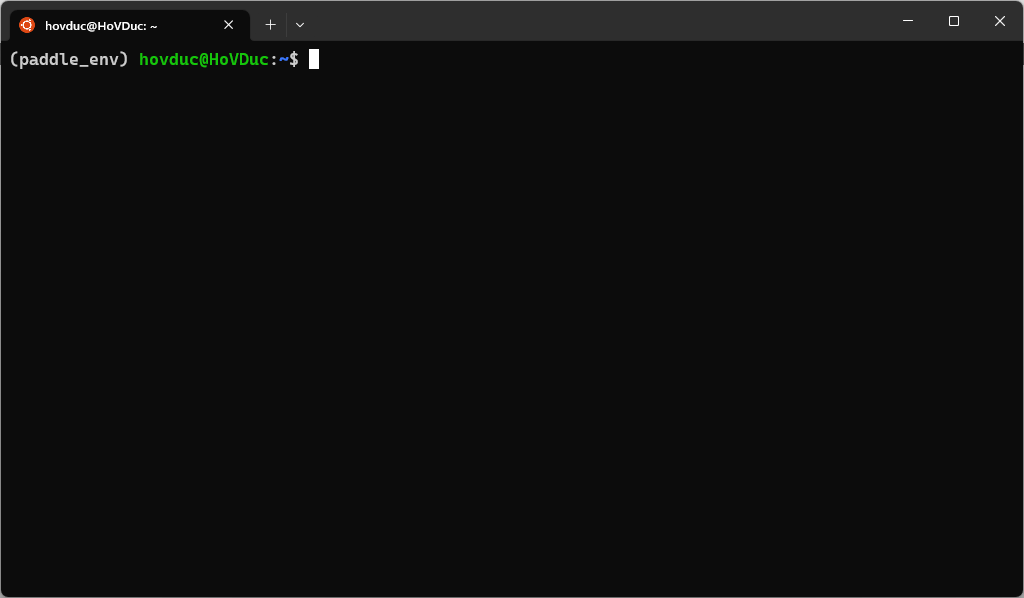
\includegraphics[scale=0.5]{images/terminal-conda-activate.png}    
    \centering
    \caption{Môi trường đã được kích hoạt}
\end{figure}

\subsection{Cài đặt CUDA Toolkit:}
\begin{lstlisting}[language=bash]
$ wget https://developer.download.nvidia.com/compute/cuda/repos/ubuntu2204/x86_64/cuda-ubuntu2204.pin
$ sudo mv cuda-ubuntu2204.pin /etc/apt/preferences.d/cuda-repository-pin-600
$ wget https://developer.download.nvidia.com/compute/cuda/11.7.0/local_installers/cuda-repo-ubuntu2204-11-7-local_11.7.0-515.43.04-1_amd64.deb
$ sudo dpkg -i cuda-repo-ubuntu2204-11-7-local_11.7.0-515.43.04-1_amd64.deb
$ sudo cp /var/cuda-repo-ubuntu2204-11-7-local/cuda-*-keyring.gpg /usr/share/keyrings/
$ sudo apt-get update
$ sudo apt-get -y install cuda
\end{lstlisting}

\subsection{Cài đặt cuDNN}
\textbf{Bước 1:} Tải xuống cuDNN
\begin{lstlisting}[language=bash]
wget https://developer.nvidia.com/downloads/compute/cudnn/secure/8.9.4/local_installers/11.x/cudnn-local-repo-ubuntu2204-8.9.4.25_1.0-1_amd64.deb
\end{lstlisting}

\textbf{Bước 2:} Cài đặt gói phần mềm
\begin{lstlisting}
sudo dpkg -i cudnn-local-repo-ubuntu2204-8.9.4.25_1.0-1_amd64.deb
\end{lstlisting}

\textbf{Bước 3:} Nhập khóa CUDA GPG
\begin{lstlisting}
sudo cp /var/cudnn-local-repo-*/cudnn-local-*-keyring.gpg /usr/share/keyrings/
\end{lstlisting}

\textbf{Bước 4:} Làm mới và cài đặt thư viện
\begin{lstlisting}
sudo apt-get update
sudo apt-get install libcudnn8=8.9.4.25_1.0-1+cuda11.7
sudo apt-get install libcudnn8-dev=8.9.4.25_1.0-1+cuda11.7
\end{lstlisting}


\subsection{Cài đặt PaddleOCR}
\textbf{Bước 1:} Cài đặt PaddlePaddle
\begin{lstlisting}[language=bash]
    python3 -m pip install paddlepaddle -i https://mirror.baidu.com/pypi/simple
\end{lstlisting}

\textbf{Bước 2:} Clone PaddleOCR và cài đặt
\begin{lstlisting}[language=bash]
    git clone https://github.com/PaddlePaddle/PaddleOCR.git
    pip install -r PaddleOCR/requirements.txt
\end{lstlisting}

\subsection{Cài đặt PPOCRLabel}
\begin{lstlisting}[language=bash]
    pip3 install PPOCRLabel
    pip3 install trash-cli
\end{lstlisting}

Trong chương này đã giới thiệu các công cụ và thư viện quan trọng trong đồ án. Phần tiếp theo em sẽ trình bày về dữ liệu và các bước huấn luyện mô hình OCR.

\newpage
\section{Kết quả}
% Chương 4 ======================================================================
\newpage
\chapter{Xây dựng chương trình và Kết quả} \label{build_and_result}

Chương này, em mô tả quá trình xây dựng một chương trình ứng dụng hoàn chỉnh cho việc nhận dạng hóa đơn thông qua công nghệ OCR và kết quả đạt được của chương trình.
\section{Phương pháp thực hiện}
Để xây dựng được một chương trình hoàn chỉnh cho đề tài ``\textbf{Nghiên cứu ứng dụng OCR nhận dạng hóa đơn}'', chương trình sẽ cần sự kết hợp của nhiều mô hình với các nhiệm vụ khác nhau để tạo thành một quy trình hoàn chỉnh. 

\begin{figure}
    \tikzstyle{terminator} = [rectangle, draw, text centered, rounded corners, minimum height=2em]
\tikzstyle{process} = [rectangle, draw, text centered, minimum height=2em]
\tikzstyle{decision} = [diamond, aspect=2, draw, text centered, minimum height=2em]
\tikzstyle{data}=[trapezium, draw, text centered, trapezium left angle=60, trapezium right angle=120, minimum height=2em]
\tikzstyle{connector} = [draw, -latex']
\tikzstyle{arrow} = [thick,->,>=stealth]
\tikzstyle{link} = [circle, draw, minimum height=0.2em]

\begin{tikzpicture}
    \node [terminator, fill=blue!5] at (0,0) (start) {\textbf{Start}};
    \node [data, fill=blue!30] at (0,-2) (data) {Image};
    \node [decision, fill=green!30] at (0,-5) (decision1) {Valid image?};
    \node [process, fill=red!20] at (5,-5) (error) {Error};
    \node [process, fill=red!20] at (-3.7,-9) (error2) {Error};
    \node [process, fill=orange!30] at (-3.5,-7) (pre-processing) {Pre-processing};
    \node [process, fill=orange!30] at (3.5,-7) (text-detection) {Text Detection};
    \node [decision, fill=green!30] at (0,-9) (decision2) {Have text?};
    \node [process, fill=orange!30] at (-3.5,-12) (recognition) {Recognition};
    \node [process, fill=orange!30] at (3.5,-12) (kie) {KIE};
    \node [process, fill=orange!30] at (0,-13) (post-process) {Post-processing};
    \node [data, fill=blue!30] at (-3.5,-16) (excel) {Excel};
    \node [data, fill=blue!30] at (3.5,-16) (visual) {Image Visualized};
    \node [link, fill=black] at (0, -18.5) (link1) {.};
    \node [link, fill=black] at (-5.7, -9) (link2) {.};

    \node [terminator, fill=blue!5] at (0,-20) (end) {\textbf{End}};
    \node[draw=none] at (3, -4.75) (no) {False};
    \node[draw=none] at (-2, -8.5) (no) {False};
    \node[draw=none] at (-4.2, -5.8) (yes) {True};
    \node[draw=none] at (-0.7, -10.5) (yes) {True};

    \path [connector] (start) -- (data);
    \path [connector] (data) -- (decision1);
    \path [connector] (decision1) -- (error);
    \path [connector] (decision1) -| (pre-processing);
    \path [connector] (pre-processing) -- (text-detection);
    \path [connector] (text-detection) |- (decision2);
    \path [connector] (decision2) -- (error2);
    \path [connector] (error2) -- (link2);
    \path [connector] (error) |- (data);

    \draw [arrow] (decision2.south) |- ++ (0, -1) -| (kie);
    \draw [arrow] (decision2.south) |- ++ (0, -1) -| (recognition);

    \path [connector] (recognition) |- (post-process);
    \path [connector] (kie) |- (post-process);

    \draw [arrow] (post-process.south) |- ++ (0, -1) -| (excel);
    \draw [arrow] (post-process.south) |- ++ (0, -1) -| (visual);

    \draw [arrow] (excel.south) |- ++ (0, -1) -| (link1.north);
    \draw [arrow] (visual.south) |- ++ (0, -1) -| (link1.north);

    \draw [arrow] (link1.east) -| ++ (-6, 0) |- (data);

    \path [connector] (link1) -- (end);
\end{tikzpicture}
    \centering
    \caption{Lưu đồ của chương trình nhận dạng hóa đơn}
    \label{pipeline}
\end{figure}

\subsection{Kiến trúc tổng quan}
Kiến trúc của chương trình Hình \ref{pipeline}, từ ảnh đầu vào bức ảnh sẽ được mô hình cho qua các hàm tiền xử lý hình ảnh để tăng chất lượng ảnh đầu vào tiếp đến ảnh sẽ được cho qua bước phát hiện văn bản để xác định vùng văn bản và bố cục của hóa đơn để mô hình nhận dạng văn bản và trích xuất thông tin chính. Bước nhận dạng sẽ dự đoán văn bản trong vùng được phát hiện còn trích xuất thông tin chính sẽ thực hiện phân loại nhãn cho vùng văn văn bản. Sau đó cả hai sẽ được qua hàm hậu xử lý để cải thiện chất lượng và độ chính xác của văn bản dễ dàng cho các bước tiếp. Trích xuất các thông tin quan trọng và trực quan hóa hình ảnh, đưa về dữ liệu có cấu trúc \ldots

\subsection{Phát hiện văn bản}
Để thực hiện phát hiện văn bản ở đây chương trình sử dụng DBNet \ref{dbnet}, Với Backbone là ResNet50 và sử dụng pre-trained là ICDAR2015, với bộ trọng số đã được huấn luyện với data hóa đơn đã được thu thập ở mục \ref{train-text-detection}, từ bức ảnh đầu vào mô hình sẽ tiến hành xác định các vùng chứa văn bản trong bức ảnh rồi thực hiện trả ra một danh sách 4 điểm tọa độ $(x, y, w, h)$ chứa văn bản bên trong đó Hình \ref{pipeline-text-detection}. 
\begin{figure}[h]
    \tikzstyle{process} = [rectangle, draw, text centered, minimum height=2em]
\tikzstyle{arrow} = [thick,->,>=stealth]
\tikzstyle{connector} = [draw, -latex']

% \node (tikzmaker) [shift={(2.5, -2.25)}] at (7,18.75) {\includegraphics[width=5cm]{áda}};
\begin{tikzpicture}
    \node [draw=none] at (-6, 4) (input-image) {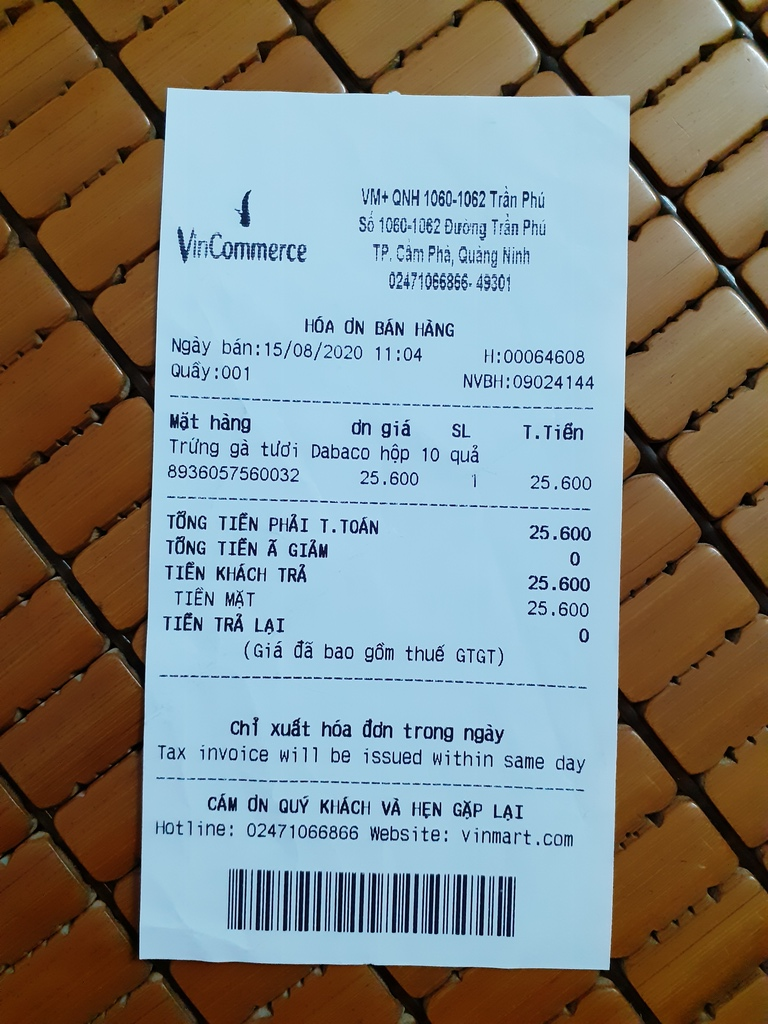
\includegraphics[scale=0.1]{chapter5/images/invoice.png}};
    \node [process] at (0, 0) (text-detection) {
        \begin{tikzpicture}
            \node [process] at (-4, 0) (cnn-fpn) {\footnotesize ResNet50 + FPN};
            \node [process] at (0, 0) (probability) {\footnotesize Probaility Map};
            \node [process] at (0, -1.5) (threshold) {\footnotesize Threshold Map};
            \node [process] at (4, -0.75) (db) {\footnotesize DB post-process};
            \node [draw=none] at (-4, -1.5) (text) {Detection};
            
            \path [connector] (cnn-fpn) -- (probability);
            \path [connector] (cnn-fpn) -- (threshold);
            \path [connector] (probability) -- (db);
            \path [connector] (threshold) -- (db);
        \end{tikzpicture}
    };
    \node [draw=none] at (6, -4) (output-image) {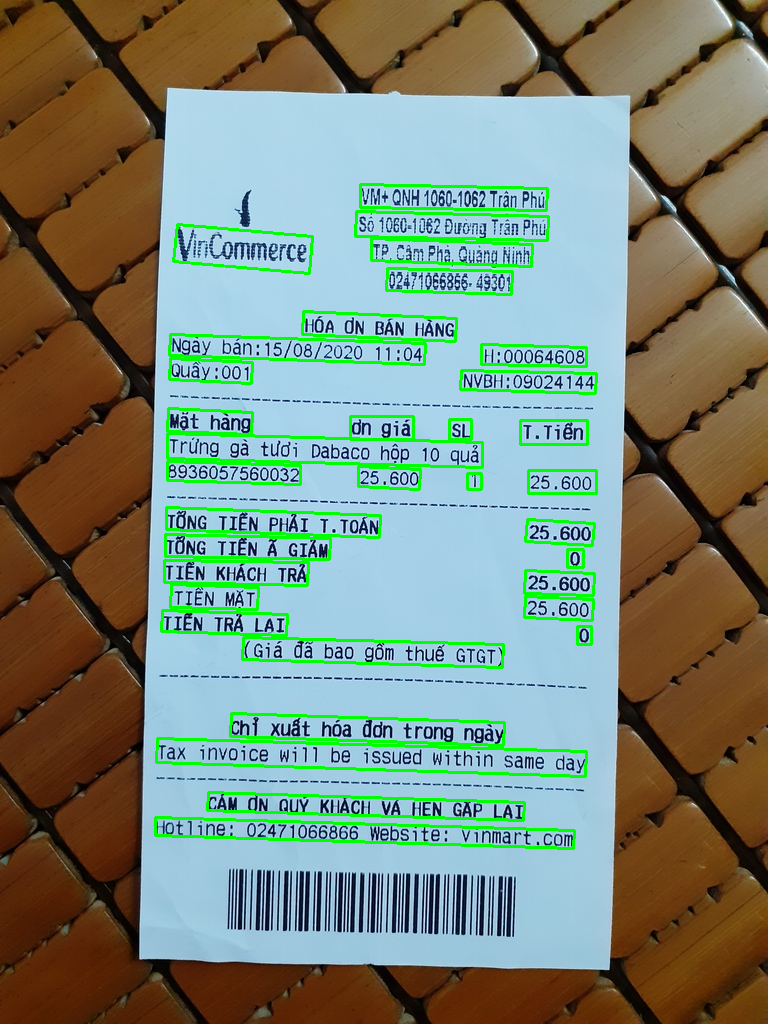
\includegraphics[scale=0.1]{chapter5/images/boudingbox-invoice.png}};

    \draw [arrow] (input-image.south) -- ++ (0, -1) |- (text-detection.west);
    \draw [arrow] (text-detection.east) -- ++ (0, 0) -| (output-image.north);
\end{tikzpicture}
    \centering
    \caption{Pipeline phát hiện văn bản}
    \label{pipeline-text-detection}
\end{figure}

\subsection{Nhận dạng văn bản} \label{method-rec}
Từ những hộp văn bản thu được từ bước phát hiện văn bản chương trình sẽ thực hiện nhận dạng văn bản. Để nhận dạng văn bản chương trình sử dụng kiến trúc của VietOCR (TransformerOCR \ref{transformerocr}) với Backbone là VGG19 được và sử dụng pre-trained là dữ liệu tiếng Việt tự phát sinh 10 triệu mẫu ảnh, và đã được huấn luyện với dữ liệu hóa đơn thu thập được ở mục \ref{train-text-recognition}, mô hình sẽ thực hiện trích xuất đặc trưng qua VGG19 đưa nó về dạng word embedding để cho qua mô-đun Transformer thu được vector xác suất. Cuối cùng sử dụng beam search để tìm kiếm các từ hoặc các ký tự phù hợp để thu được kết quả cuối cùng hình \ref{pipeline-text-recognition}.
\begin{figure}[h]
    \tikzstyle{process} = [rectangle, draw, text centered, minimum height=2em]
\tikzstyle{arrow} = [thick,->,>=stealth]
\tikzstyle{connector} = [draw, -latex']

\begin{tikzpicture}
    \node [draw=none] at (-5, 1.5) (input-image) {
\includegraphics[scale=0.6]{chapter5/images/text-image.png}};
    \node [draw=none] at (-6, 0) (input) {input};
    \node[process] at (0, 0) (box) {
        \begin{tikzpicture}
            \node [process] at (-3.5, 0) (cnn) {\footnotesize VGG19};
            \node [process] at (0, 0) (transformer) {\footnotesize Transformer};
            \node [process] at (4, 0) (beamsearch) {\footnotesize Beam Search};

            \path [connector] (cnn) -- (transformer);
            \path [connector] (transformer) -- (beamsearch);
        \end{tikzpicture}
    };
    \node [draw=none] at (6, 0) (output) {output};
    \node [draw=none] at (5, -1.5) (input-image) {\footnotesize VM+ QNH 1060-1062 Trần Phú};

    \path [connector] (input) -- (box);
    \path [connector] (box) -- (output);
\end{tikzpicture}
    \centering
    \caption{Pipeline nhận dạng văn bản}
    \label{pipeline-text-recognition}
\end{figure}

\subsection{Key information extraction}
Còn đối với mô-đun Trích xuất thông tin chính thực hiện song song với \ref{method-rec}, mô-đun này sử dụng mô hình LayoutXLM cùng với pre-trained được huấn luyện trên bộ dataset XFUND. Bộ trọng số của mô hình này đã được huấn luyện với dữ liệu hóa đơn đã thu thập được ở mục \ref{training-kie}. Mô-đun này sẽ sử dụng thông tin hình ảnh, văn bản và bố cục của hóa đơn mã hóa chúng về dạng embedding, embedding văn bản và hình ảnh được nối lại với nhau và cộng với embedding bố cục để thu được embedding đầu vào. Embedding này sẽ được cho qua mô hình Multi-Modal Transformer để thực hiện phân loại thông tin trong tờ hóa đơn (Hình \ref{pipeline-kie}).
\begin{figure}
    \tikzstyle{process} = [rectangle, draw, text centered, minimum height=2em]
\tikzstyle{arrow} = [thick,->,>=stealth]
\tikzstyle{connector} = [draw, -latex']

\begin{tikzpicture}
    \node [draw=none] at (0, 0) (input) {input};
    \node [draw=none] at (5, 2.1) (none) {\scriptsize ocr system};
    \node [draw=none, rotate=22] at (1.5, 0.8) (none) {\scriptsize image};
    \node [draw=none, rotate=0] at (1.5, 0.15) (none) {\scriptsize text};
    \node [draw=none, rotate=345] at (3.5, -1.0) (none) {\scriptsize layout};
    \node [process] at (5, 1.25) (image) {Image Embedding};
    \node [process] at (5, 0) (text) {Text Embedding};
    \node [process] at (8, -2) (layout) {Layout Embedding};
    \draw [, dashed] (3, 2.5) rectangle (7, -0.5);
    \node [process, rotate=90] at (9, 1) (concat) {Concat};
    \node [draw=none] at (9, -0.75) (no) {\Large $\oplus $};
    \node [process, rotate=90] at (12, 0) (model) {Multi-modal Transformer};
    \node [draw=none] at (14, 0) (output) {output};

    \path [connector] (input) -- (image.west);
    \path [connector] (input) -- (text);
    \path [connector] (input) -- (layout.west);
    \path [connector] (image.east) -- (concat);
    \path [connector] (text.east) -- (concat);
    \path [connector] (concat) -- (model);
    \path [connector] (layout.east) -- (model);
    \path [connector] (model) -- (output);
\end{tikzpicture}
    \centering
    \caption{Pipeline trích xuất thông tin chính}
    \label{pipeline-kie}
\end{figure}
\newpage
\section{Xây dựng chương trình}
\subsection{Tiền xử lý ảnh}

\begin{lstlisting}[language=Python]
def preprocess_image(_image):
    _image = alpha_to_color(_image, alpha_color)

    # Image Sharpness
    kernel = np.array([[-1,-1,-1], 
                       [-1, 9,-1], 
                       [-1,-1,-1]])
    _image = cv2.filter2D(_image, -1, kernel)
    if inv:
        _image = cv2.bitwise_not(_image)
    if bin:
        _image = binarize_img(_image)
    return _image  
\end{lstlisting}

Ở đoạn code trên em sử dụng các phương pháp tiền xử lý ảnh cơ bản, để cải thiện chất lượng ảnh đầu vào cho chương trình.
\subsection{Phát hiện vùng văn bản} \label{detsec}
Đoạn code dưới đây sử dụng thư viện PaddleOCR để xây dựng một ứng dụng phát hiện văn bản trong hình ảnh.
\begin{lstlisting}[language=Python]
from paddleocr import PaddleOCR

self.ocr_engine = PaddleOCR(
    use_angle_cls=False,
    show_log=False,
    det_model_dir=global_config.get("kie_det_model_dir", None),
    use_gpu=global_config['use_gpu'])

det_result = self.ocr_engine(image)
\end{lstlisting}
Kết quả trả về là một danh sách các điểm tọa độ
\begin{lstlisting}[language=Python]
[[27.0, 459.0], [136.0, 459.0], [136.0, 479.0], [27.0, 479.0]]
[[28.0, 429.0], [372.0, 429.0], [372.0, 445.0], [28.0, 445.0]]
......
\end{lstlisting}

\subsection{Nhận dạng văn bản}
Với nhận dạng hóa đơn đầu vào của nhiệm vụ này là kết quả của \ref{detsec}. Hàm \texttt{recog} nhận 2 tham số đầu vào là ảnh đầu vào, và các điểm tọa độ, hàm sẽ thực hiện lấy các vùng văn bản và thực hiện dự đoán các văn bản trong từng \texttt{roi}.
\begin{lstlisting}[language=Python]
from src.ocr.tools.predictor import Predictor
from src.ocr.tools.config import Cfg

self.config = Cfg.load_config_from_file(global_config['rec_config_path'])
self.config['predictor']['import'] = global_config['rec_weight']
self.config['predictor']['beamsearch'] = True
self.config['cnn']['pretrained'] = False
self.config['device'] = 'cuda' if global_config['use_gpu'] else 'cpu'
self.detector = Predictor(self.config)

def recog(image, boxes):
    texts = []
    for box in tqdm(boxes):
        x, y, w, h = box
        roi = Image.fromarray(image[y:h, x:w])
        text = self.detector.predict(roi)
        texts.append(text)
    return text

self.recog(image, det_result)

\end{lstlisting}

Kết quả trả về của nhiệm vụ này là list các văn bản đã được dự đoán như hình dưới đây.
\begin{lstlisting}[language=Python]
['Okono', 'Số 85 Lê Văn Hiến, Đức Thắng, Bắc Từ Liêm', 'PHIÊU BÁN HÀNG/ INVOICE', 'Số:A3 1AA145550Ngày:18/05/2023 7:51:19PM', ...]
\end{lstlisting}
\subsection{KIE}
Đoạn mã sau thực hiện quy trình dự đoán phân loại thông tin trong hình ảnh, từ việc chuẩn bị dữ liệu đến việc thực hiện dự đoán và xử lý kết quả sau khi dự đoán.
\begin{lstlisting}[language=Python]
from ppocr.data import create_operators, transform
from ppocr.modeling.architectures import build_model
from ppocr.postprocess import build_post_process

self.post_process_class = build_post_process(config['PostProcess'],
                                             global_config)
self.model = build_model(config['Architecture'])

transforms = []
for op in config['Eval']['dataset']['transforms']:
    op_name = list(op)[0]
    if 'Label' in op_name:
        op[op_name]['ocr_engine'] = self.ocr_engine
    elif op_name == 'KeepKeys':
        op[op_name]['keep_keys'] = [
            'input_ids', 'bbox', 'attention_mask', 'token_type_ids',
            'image', 'labels', 'segment_offset_id', 'ocr_info',
            'entities'
        ]
    transforms.append(op)

if config["Global"].get("infer_mode", None) is None:
    global_config['infer_mode'] = True
self.ops = create_operators(config['Eval']['dataset']['transforms'],
                            global_config)
self.model.eval()

batch = transform(data, self.ops)
batch = to_tensor(batch)
preds = self.model(batch)
post_result = self.post_process_class(
            preds, segment_offset_ids=batch[6], ocr_infos=batch[7])
\end{lstlisting}
Kết quả sẽ trả về một danh sách các dictionary như sau:
\begin{lstlisting}[language=Python]
[[{'transcription': 'Okono', 'bbox': [435, 195, 811, 338], 'points': [[437.0, 195.0], [811.0, 201.0], [808.0, 338.0], [435.0, 332.0]], 'pred_id': 1, 'pred': 'SELLER'}, {'transcription': 'Số 85 Lê Văn Hiến, Đức Thắng, Bắc Từ Liêm', 'bbox': [309, 390, 890, 426], 'points': [[309.0, 390.0], [890.0, 392.0], [890.0, 426.0], [309.0, 424.0]], 'pred_id': 3, 'pred': 'ADDRESS'},...]
\end{lstlisting}
\subsection{Post-process}
Đoạn mã sau có chức năng xử lý và trích xuất thông tin từ kết quả của quá trình nhận dạng hóa đơn, sau đó tạo một Pandas DataFrame để lưu trữ thông tin này và xuất ra một tệp Excel

\begin{lstlisting}[language=Python]
def process_info(self, results):
    info = {
        'SELLER': '',
        'ADDRESS': '',
        'STAFF': '',
        'TIMESTAMP': '',
        'CODE': '',
        'PRODUCTS': [],
        'TOTAL_COST': 0
    }
    
    current_product = {
        'PRODUCT': '',
        'NUMBER': 0,
        'PRICE': 0
    }
    
    products = []
    for result in results:
        label = result['pred']
        transcription = result['transcription']
        
        if label != 'O':
            if label in ['PRODUCT', 'NUMBER', 'PRICE']:
                if label == 'PRODUCT':
                    current_product['PRODUCT'] = transcription
                    products.append(current_product.copy())
                else:
                    products[-1][label] = transcription
            else: 
                if label == 'TIMESTAMP':
                    text = transcription
                    code, time = text.split('Ngày')
                    info['CODE'] = code.strip()
                    info['TIMESTAMP'] = time[1:]
                else:
                    info[label] = transcription
                    
    info['PRODUCTS'] = products 

    product_rows = []
    for product in info_["PRODUCTS"]:
        product_row = [info_["SELLER"], info_["ADDRESS"], info_["STAFF"], info_["TIMESTAMP"], info_["CODE"],
                    product["PRODUCT"], product["NUMBER"], product["PRICE"], info_["TOTAL_COST"]]
        product_rows.append(product_row)

    # Create a Pandas DataFrame
    columns = ["SELLER", "ADDRESS", "STAFF", "TIMESTAMP", "CODE", "PRODUCT", "NUMBER", "PRICE", "TOTAL_COST"]
    df = pd.DataFrame(product_rows, columns=columns)

    # Create an Excel file
    now = datetime.now()

    current_time = now.strftime("%H-%M-%S")
    output_file = "invoice-{}.xlsx".format(current_time)
    df.to_excel(output_file, index=False, engine="openpyxl")

    print(f"Excel file '{output_file}' created.")

    return json.dumps(info, indent=1, ensure_ascii=False)
\end{lstlisting}

Đoạn mã sau vẽ kết quả của chương trình lên trên hình ảnh gốc.
\begin{lstlisting}[language=Python]
def draw_ser_results(image, ocr_results, 
                     font_path="doc/fonts/BeVietnamPro-Black.ttf", font_size=14):
    np.random.seed(2021)
    color = (np.random.permutation(range(255)),
             np.random.permutation(range(255)),
             np.random.permutation(range(255)))
    color_map = {
        idx: (color[0][idx], color[1][idx], color[2][idx])
        for idx in range(1, 255)
    }
    if isinstance(image, np.ndarray):
        image = Image.fromarray(image)
    elif isinstance(image, str) and os.path.isfile(image):
        image = Image.open(image).convert('RGB')
    img_new = image.copy()
    draw = ImageDraw.Draw(img_new)

    font = ImageFont.truetype(font_path, font_size, encoding="utf-8")
    for ocr_info in ocr_results:
        if ocr_info["pred_id"] not in color_map:
            continue
        color = color_map[ocr_info["pred_id"]]
        text = "{}: {}".format(ocr_info["pred"], ocr_info["transcription"])

        if "bbox" in ocr_info:
            bbox = ocr_info["bbox"]
        else:
            bbox = trans_poly_to_bbox(ocr_info["points"])
        draw_box_txt(bbox, text, draw, font, font_size, color)

    img_new = Image.blend(image, img_new, 0.7)
    return np.array(img_new)    
\end{lstlisting}

\newpage
\section{Kết quả}
Dưới đây là một số kết quả đạt được của đề tài trên bộ dữ liệu hóa đơn Okono và Vincommerce:
\paragraph*{Kết quả 1}
\begin{figure}[h]
    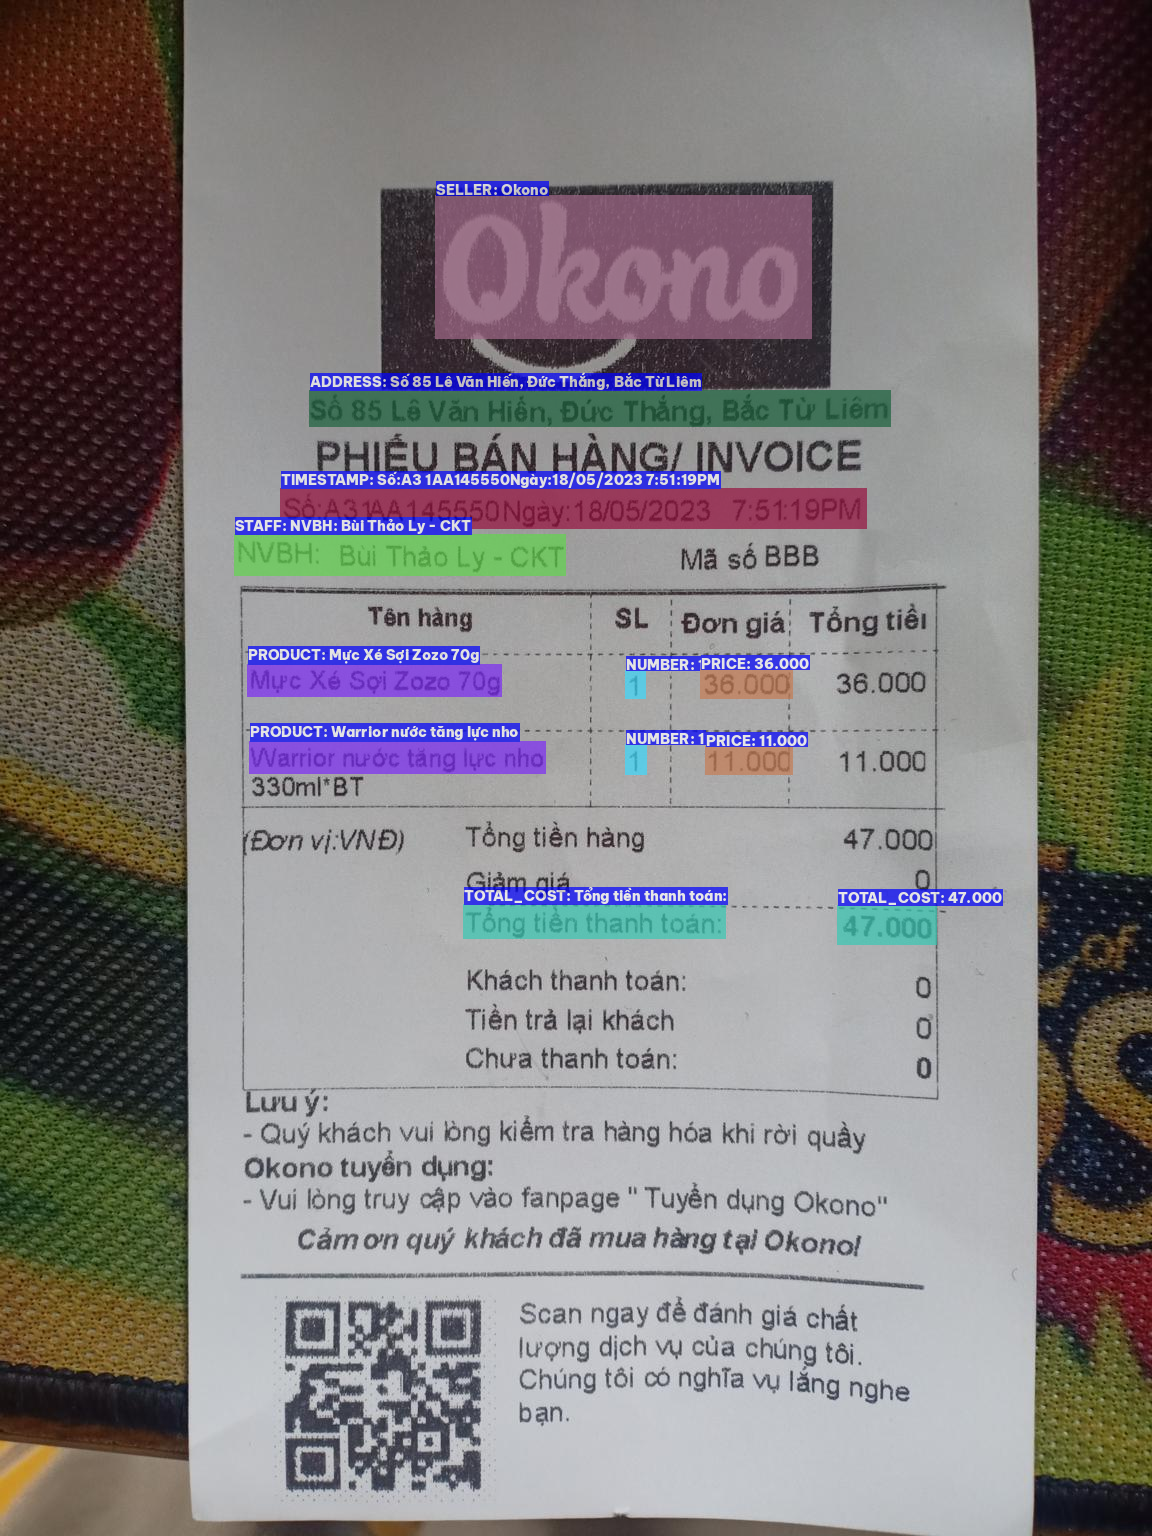
\includegraphics[scale=0.2]{images/dem-image.png}
    \centering
    \caption{Kết quả hình ảnh hóa đơn 1}
\end{figure}

\begin{lstlisting}[language=Python]
{
    "SELLER": "Okono",
    "ADDRESS": "Số 85 Lê Văn Hiến, Đức Thắng, Bắc Từ Liêm",
    "STAFF": "NVBH: Bùi Thảo Ly - CKT",
    "TIMESTAMP": "18/05/2023 7:51:19PM",
    "CODE": "Số:A3 1AA145550",
    "PRODUCTS": [
        {
        "PRODUCT": "Mực Xé Sợi Zozo 70g",
        "NUMBER": "1",
        "PRICE": "36.000"
        },
        {
        "PRODUCT": "Warrior nước tăng lực nho",
        "NUMBER": "1",
        "PRICE": "11.000"
        }
    ],
    "TOTAL_COST": "47.000"
}
\end{lstlisting}

\begin{figure}[h]
    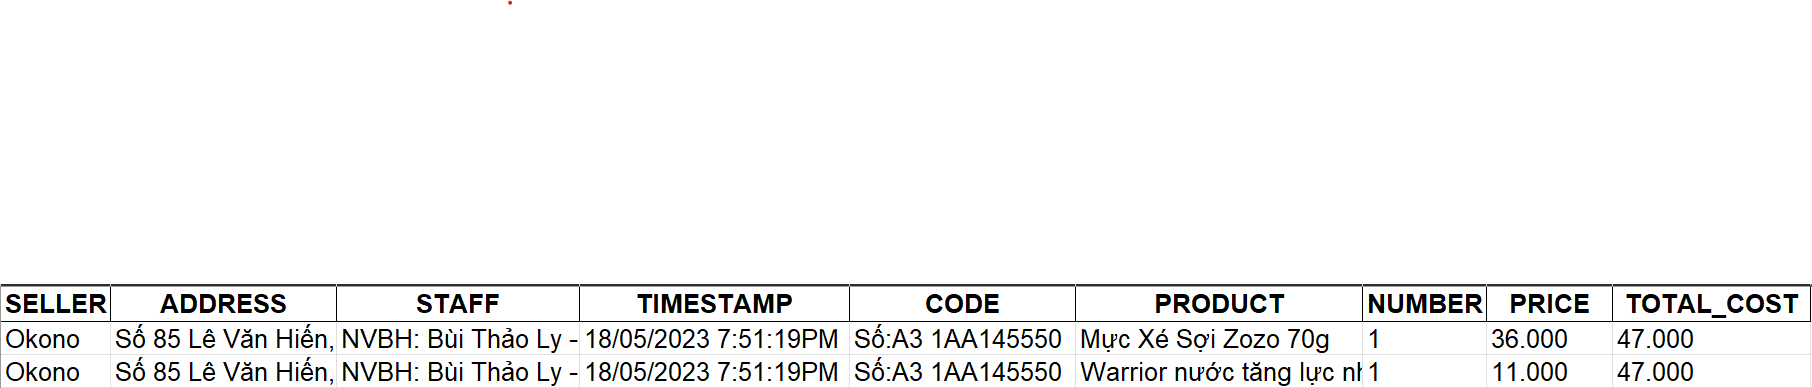
\includegraphics[scale=0.312]{images/result-demi-1.png}
    \caption{Kết quả Excel của hóa đơn 1}
\end{figure}

\paragraph*{Kết quả 2}
\begin{figure}[h]
    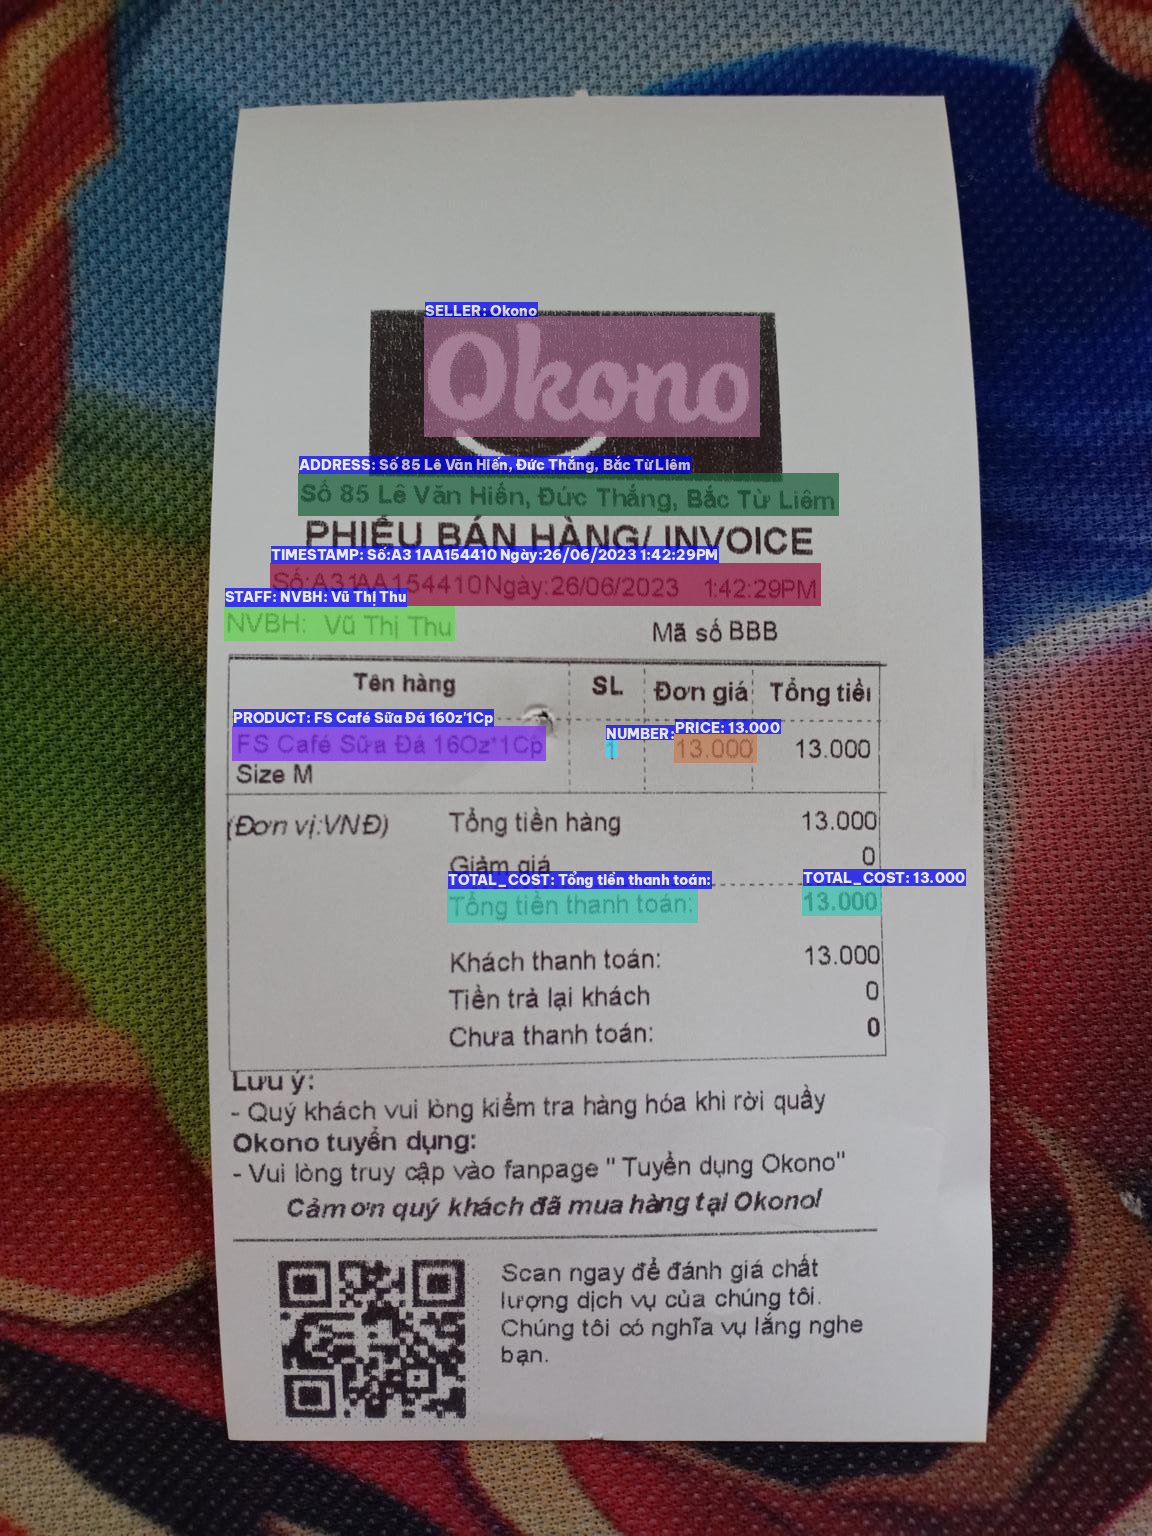
\includegraphics[scale=0.2]{images/demo-image-1.png}
    \centering
    \caption{Kết quả hình ảnh hóa đơn 2}
\end{figure}

\begin{lstlisting}[language=Python]
{
    "SELLER": "Okono",
    "ADDRESS": "Số 85 Lê Văn Hiến, Đức Thắng, Bắc Từ Liêm",
    "STAFF": "NVBH: Vũ Thị Thu",
    "TIMESTAMP": "26/06/2023 1:42:29PM",
    "CODE": "Số:A3 1AA154410",
    "PRODUCTS": [
        {
        "PRODUCT": "FS Café Sữa Đá 160z'1Cp",
        "NUMBER": "1",
        "PRICE": "13.000"
        }
    ],
    "TOTAL_COST": "13.000"
}
\end{lstlisting}

\begin{figure}[h]
    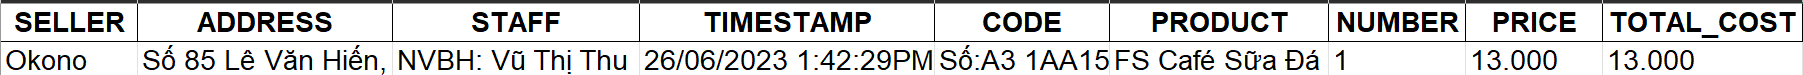
\includegraphics[scale=0.314]{images/result-demo-excel-2.png}
    \caption{Kết quả Excel của hóa đơn 2}
\end{figure}

\paragraph*{Kết quả 3}
\begin{figure}[h]
    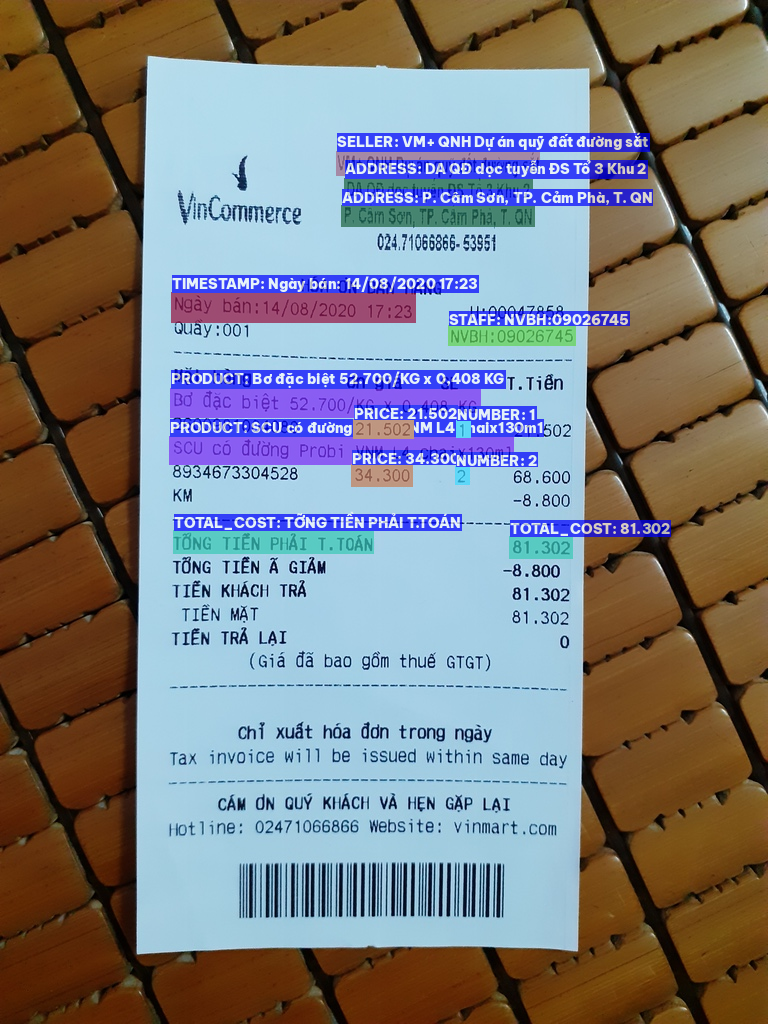
\includegraphics[scale=0.3]{images/demo-image-3.png}
    \centering
    \caption{Kết quả hình ảnh hóa đơn 3}
\end{figure}

\begin{lstlisting}[language=Python]
{
    "SELLER": "VM+ QNH Dự án quỹ đất đường sắt",
    "ADDRESS": "P. Câm Sơn, TP. Cảm Phà, T. QN",
    "STAFF": "NVBH:09026745",
    "TIMESTAMP": "14/08/2020 17:23",
    "CODE": "",
    "PRODUCTS": [
        {
        "PRODUCT": "Bơ đặc biệt 52.700/KG x 0,408 KG",
        "NUMBER": 0,
        "PRICE": 0
        },
        {
        "PRODUCT": "SCU có đường Probi VNM L4 chaix130m1",
        "NUMBER": "2",
        "PRICE": "34.300"
        }
    ],
    "TOTAL_COST": "81.302"
    }
}
\end{lstlisting}

\begin{figure}[h]
    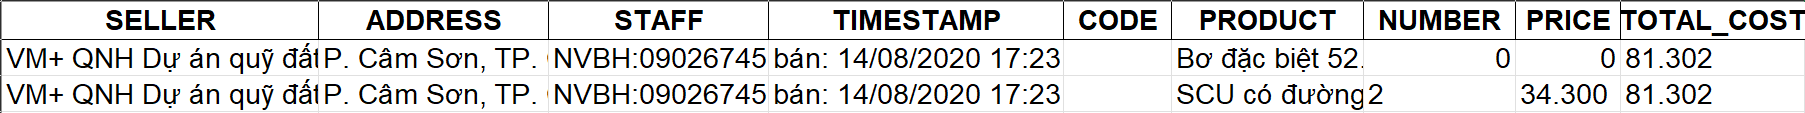
\includegraphics[scale=0.314]{images/result-demo-excel-3.png}
    \caption{Kết quả Excel của hóa đơn 3}
\end{figure}
Qua kết quả trên chương trình đã đạt được hiệu quả tốt trên bộ dữ liệu thu thập được với kết quả trên từng tác vụ đã được ở trình bày ở bảng \ref{table:1}. 

Với những thông tin thu được từ hóa đơn như ở trên em tin rằng điều này sẽ giúp cho doanh nghiệp, hay cá nhân người sử dụng có thể lưu trữ và quản lý thông tin hóa đơn một cách hiệu quả cho đối tượng cụ thể. Những thông tin đó có thể giúp cho người sử dụng có thể dễ dàng quản lý, tránh thất thoát sản phẩm, nguồn hàng, quản lý tài chính, nếu xảy ra sai xót trong quá trình mua bán có thể truy tìm, nguồn gốc sai xót \dots

Điều này đã kết thúc chương \ref{build_and_result}, trong chương này em đã mô tả quá trình xây dựng chương trình hoàn chỉnh của đề tài bao gồm kết quả của chương trình. Kết quả đạt được của chương trình cho người dùng có một cái nhìn tổng quát về những gì mà mô hình trích xuất, và thông tin hóa đơn được chương trình lưu trữ lại dưới dạng dữ liệu có cấu trúc. 

% Chương 5 ======================================================================
\newpage
\section*{\Large\centering Kết luận}{}
\addcontentsline{toc}{chapter}{Kết luận}
Sau quá trình nghiên cứu và tìm hiểu các phương pháp, thuật toán liên quan đến OCR cùng với sự nỗ lực của bản thân em đã hoàn thành đề tài kịp tiến độ đề tài ``\textbf{Nghiên cứu ứng dụng công nghệ OCR nhận dạng hóa đơn}'' và đạt được những kết quả sau:
\begin{enumerate}
    \item Tìm hiểu và áp dụng thành công các thuật toán ``state-of-the-art'' cho đề tài
    \item Huấn luyện thành công các mô hình cho nhiệm vụ khác nhau phát hiện văn bản, nhận dạng văn bản, \acrshort*{kie} và đạt hiệu quả tốt trên bộ dữ liệu thu thập được.
    \item Xây dựng hoàn chỉnh chương trình trích xuất thông tin hóa đơn.
    \item Thành công chuyển đổi ảnh hóa đơn thành dạng văn bản có thể xử lý được.
    \item Trích xuất được các thông tin quan trọng của hóa đơn như tên cửa hàng, địa chỉ, ngày mua, sản phẩm, \ldots Và lưu trữ thông tin dưới dạng văn bản có cấu trúc. 
\end{enumerate}

Như vậy, đề tài đã hoàn thành mục tiêu đề ra và đạt được những kết quả quan trọng trong việc ứng dụng công nghệ OCR để nhận dạng và trích xuất thông tin từ hóa đơn.

\subsection*{Những hạn chế của đề tài} \label{hanche}
Tuy vậy, đề tài còn một số hạn chế đáng chú ý như sau:
\begin{enumerate}
    \item Dễ ảnh hưởng bởi nhiều yếu tố như chất lượng hình ảnh, font chữ, định dạng
    hóa đơn
    \item Mô-đun phát hiện văn bản vẫn chưa phát hiện được hầu hết văn bản. Điều này đẫn đến thiếu xót thông tin trong quá trình nhận diện và trích xuất thông tin.
    \item Mô-đun nhận diện văn bản, dễ bị ảnh hưởng bởi chất lượng hình ảnh, và nhiễu. Điều này làm cho quá trình nhận dạng trở lên sai xót ảnh hưởng đến thông tin lưu trữ.
    \item Mẫu hóa đơn chưa được đa dạng và phong phú, chỉ nhận dạng trên vào mẫu hóa đơn nhất định.
\end{enumerate}

\subsection*{Hướng phát triển}
Trong tương lai, Em sẽ tiếp tục tìm hiểu và nghiên cứu thêm để khắc phục các vấn đề còn tồn tại của đề tài. Phát triển và mở rộng phạm vi nghiên cứu nhằm phát triển các kỹ năng và kiến thức để cải thiện bản thân. Dưới đây là những dự định phát triển:
\begin{enumerate}
    \item Khắc phục các hạn chế ở mục hạn chế, tối ưu hóa độ chính xác, thời gian chạy và đa dạng mẫu hóa đơn ,và cải thiện khả năng nhận dạng trong các trường hợp phức tạp.
    \item Xây dựng ứng dụng di động cho phép người dùng chụp ảnh hóa đơn bằng điện thoại di động và tự động đưa ra thông tin liên quan. Điều này sẽ giúp tạo ra một trải nghiệm tiện lợi và linh hoạt cho người dùng.
    \item Tích hợp ứng dụng OCR vào hệ thống quản lý tài liệu và dữ liệu của doanh nghiệp. Điều này sẽ giúp tự động hóa quy trình làm việc, giảm thiểu thời gian và nguy cơ sai sót trong việc nhập liệu thủ công.
\end{enumerate}

Trải qua quá trình nghiên cứu và thử nghiệm, Em nhận thấy rằng OCR có tiềm năng lớn trong việc tối ưu hóa quá trình nhận dạng và nhập liệu từ hóa đơn. Nhờ vào việc tự động nhận dạng ký tự, giảm thiểu sự phụ thuộc vào công việc thủ công, giảm nguy cơ sai sót từ việc nhập liệu thủ công và tăng khả năng đáp ứng nhanh chóng các yêu cầu kinh doanh.

Tổng kết lại, ``nghiên cứu về ứng dụng OCR trong nhận dạng hóa đơn'' là một bước tiến quan trọng trong việc áp dụng công nghệ vào thực tiễn kinh doanh. Tin rằng sự phát triển của OCR cùng với sự tương tác với các công nghệ khác sẽ mở ra những cơ hội mới và đóng góp tích cực cho sự phát triển của nền kinh tế và xã hội.






\newpage
\addcontentsline{toc}{chapter}{Tài Liệu Tham Khảo}
\printbibliography[heading=talikarng]
\end{document}